\documentclass[11pt]{article}%
\usepackage{geometry}%
\geometry{a4paper,
  lmargin=2cm,rmargin=2cm,tmargin=2.5cm,bmargin=2.5cm}

\usepackage{array}
\usepackage{paralist}

\usepackage[svgnames, usenames, dvipsnames]{xcolor}
\xdefinecolor{RecColor}{named}{Aqua}
\xdefinecolor{IncColor}{named}{Aqua}
\xdefinecolor{ImpColor}{named}{PaleGreen}

% \usepackage{frcursive}

\usepackage{adjustbox}

%%%%%%%%%%%
\newcommand{\cRB}[1]{{\color{Red} \pmb{#1}}} %
\newcommand{\cR}[1]{{\color{Red} {#1}}} %
\newcommand{\cBB}[1]{{\color{Blue} \pmb{#1}}}
\newcommand{\cB}[1]{{\color{Blue} {#1}}}
\newcommand{\cGB}[1]{{\color{LimeGreen} \pmb{#1}}}
\newcommand{\cG}[1]{{\color{LimeGreen} {#1}}}

%%%%%%%%%%

\usepackage{diagbox} %
\usepackage{colortbl} %
\usepackage{multirow} %
\usepackage{pgf} %
\usepackage{environ} %
\usepackage{fancybox} %
\usepackage{textcomp} %
\usepackage{marvosym} %

%%%%%%%%%% pour qu'une cellcolor ne recouvre pas le trait du tableau
\usepackage{hhline}%

\usepackage{pgfplots}
\pgfplotsset{compat=1.10}
\usepgfplotslibrary{patchplots}
\usepgfplotslibrary{fillbetween}
\usepackage{tikz,tkz-tab}
\usepackage{ifthen}
\usepackage{calc}
\usetikzlibrary{calc,decorations.pathreplacing,arrows,positioning} 
\usetikzlibrary{fit,shapes,backgrounds}
\usepackage[nomessages]{fp}% http://ctan.org/pkg/fp

\usetikzlibrary{matrix,arrows,decorations.pathmorphing,
  decorations.pathreplacing} 

\newcommand{\myunit}{1 cm}
\tikzset{
    node style sp/.style={draw,circle,minimum size=\myunit},
    node style ge/.style={circle,minimum size=\myunit},
    arrow style mul/.style={draw,sloped,midway,fill=white},
    arrow style plus/.style={midway,sloped,fill=white},
}

%%%%%%%%%%%%%%
%%%%% écrire des inférieur égal ou supérieur égal avec typographie
%%%%% francaise
%%%%%%%%%%%%%

\renewcommand{\geq}{\geqslant}
\renewcommand{\leq}{\leqslant}
\renewcommand{\emptyset}{\varnothing}

\newcommand{\Leq}{\leqslant}
\newcommand{\Geq}{\geqslant}

%%%%%%%%%%%%%%
%%%%% Macro Celia
%%%%%%%%%%%%%

\newcommand{\ff}[2]{\left[#1, #2\right]} %
\newcommand{\fo}[2]{\left[#1, #2\right[} %
\newcommand{\of}[2]{\left]#1, #2\right]} %
\newcommand{\soo}[2]{\left]#1, #2\right[} %
\newcommand{\abs}[1]{\left|#1\right|} %
\newcommand{\Ent}[1]{\left\lfloor #1 \right\rfloor} %


%%%%%%%%%%%%%%
%%%%% tikz : comment dessiner un "oeil"
%%%%%%%%%%%%%

\newcommand{\eye}[4]% size, x, y, rotation
{ \draw[rotate around={#4:(#2,#3)}] (#2,#3) -- ++(-.5*55:#1) (#2,#3)
  -- ++(.5*55:#1); \draw (#2,#3) ++(#4+55:.75*#1) arc
  (#4+55:#4-55:.75*#1);
  % IRIS
  \draw[fill=gray] (#2,#3) ++(#4+55/3:.75*#1) arc
  (#4+180-55:#4+180+55:.28*#1);
  % PUPIL, a filled arc
  \draw[fill=black] (#2,#3) ++(#4+55/3:.75*#1) arc
  (#4+55/3:#4-55/3:.75*#1);%
}


%%%%%%%%%%
%% discontinuité fonction
\newcommand\pointg[2]{%
  \draw[color = red, very thick] (#1+0.15, #2-.04)--(#1, #2-.04)--(#1,
  #2+.04)--(#1+0.15, #2+.04);%
}%

\newcommand\pointd[2]{%
  \draw[color = red, very thick] (#1-0.15, #2+.04)--(#1, #2+.04)--(#1,
  #2-.04)--(#1-0.15, #2-.04);%
}%

%%%%%%%%%%
%%% 1 : position abscisse, 2 : position ordonnée, 3 : taille, 4 : couleur
%%%%%%%%%%
% \newcommand\pointG[4]{%
%   \draw[color = #4, very thick] (#1+#3, #2-(#3/3.75))--(#1,
%   #2-(#3/3.75))--(#1, #2+(#3/3.75))--(#1+#3, #2+(#3/3.75)) %
% }%

\newcommand\pointG[4]{%
  \draw[color = #4, very thick] ({#1+#3/3.75}, {#2-#3})--(#1,
  {#2-#3})--(#1, {#2+#3})--({#1+#3/3.75}, {#2+#3}) %
}%

\newcommand\pointD[4]{%
  \draw[color = #4, very thick] ({#1-#3/3.75}, {#2+#3})--(#1,
  {#2+#3})--(#1, {#2-#3})--({#1-#3/3.75}, {#2-#3}) %
}%

\newcommand\spointG[4]{%
  \draw[color = #4, very thick] ({#1+#3/1.75}, {#2-#3})--(#1,
  {#2-#3})--(#1, {#2+#3})--({#1+#3/1.75}, {#2+#3}) %
}%

\newcommand\spointD[4]{%
  \draw[color = #4, very thick] ({#1-#3/2}, {#2+#3})--(#1,
  {#2+#3})--(#1, {#2-#3})--({#1-#3/2}, {#2-#3}) %
}%

%%%%%%%%%%

\newcommand{\Pb}{\mathtt{P}}

%%%%%%%%%%%%%%%
%%% Pour citer un précédent item
%%%%%%%%%%%%%%%
\newcommand{\itbf}[1]{{\small \bf \textit{#1}}}


%%%%%%%%%%%%%%%
%%% Quelques couleurs
%%%%%%%%%%%%%%%

\xdefinecolor{cancelcolor}{named}{Red}
\xdefinecolor{intI}{named}{ProcessBlue}
\xdefinecolor{intJ}{named}{ForestGreen}

%%%%%%%%%%%%%%%
%%%%%%%%%%%%%%%
% barrer du texte
\usetikzlibrary{shapes.misc}

\makeatletter
% \definecolor{cancelcolor}{rgb}{0.127,0.372,0.987}
\newcommand{\tikz@bcancel}[1]{%
  \begin{tikzpicture}[baseline=(textbox.base), inner sep=0pt]
    \node[strike out, draw] (textbox) {#1}[thick, color=cancelcolor];
    \useasboundingbox (textbox);
  \end{tikzpicture}%
}
\newcommand{\bcancel}[1]{%
  \relax\ifmmode
    \mathchoice{\tikz@bcancel{$\displaystyle#1$}}
               {\tikz@bcancel{$\textstyle#1$}}
               {\tikz@bcancel{$\scriptstyle#1$}}
               {\tikz@bcancel{$\scriptscriptstyle#1$}}
  \else
    \tikz@bcancel{\strut#1}%
  \fi
}
\newcommand{\tikz@xcancel}[1]{%
  \begin{tikzpicture}[baseline=(textbox.base),inner sep=0pt]
  \node[cross out,draw] (textbox) {#1}[thick, color=cancelcolor];
  \useasboundingbox (textbox);
  \end{tikzpicture}%
}
\newcommand{\xcancel}[1]{%
  \relax\ifmmode
    \mathchoice{\tikz@xcancel{$\displaystyle#1$}}
               {\tikz@xcancel{$\textstyle#1$}}
               {\tikz@xcancel{$\scriptstyle#1$}}
               {\tikz@xcancel{$\scriptscriptstyle#1$}}
  \else
    \tikz@xcancel{\strut#1}%
  \fi
}
\makeatother

\newcommand{\xcancelRA}{\xcancel{\rule[-.15cm]{0cm}{.5cm} \Rightarrow
    \rule[-.15cm]{0cm}{.5cm}}}

%%%%%%%%%%%%%%%%%%%%%%%%%%%%%%%%%%%
%%%%%%%%%%%%%%%%%%%%%%%%%%%%%%%%%%%

\newcommand{\vide}{\multicolumn{1}{c}{}}

%%%%%%%%%%%%%%%%%%%%%%%%%%%%%%%%%%%
%%%%%%%%%%%%%%%%%%%%%%%%%%%%%%%%%%%


\usepackage{multicol}
% \usepackage[latin1]{inputenc}
% \usepackage[T1]{fontenc}
\usepackage[utf8]{inputenc}
\usepackage[T1]{fontenc}
\usepackage[normalem]{ulem}
\usepackage[french]{babel}

\usepackage{url}    
\usepackage{hyperref}
\hypersetup{
  backref=true,
  pagebackref=true,
  hyperindex=true,
  colorlinks=true,
  breaklinks=true,
  urlcolor=blue,
  linkcolor=black,
  %%%%%%%%
  % ATTENTION : red changé en black pour le Livre !
  %%%%%%%%
  bookmarks=true,
  bookmarksopen=true
}

%%%%%%%%%%%%%%%%%%%%%%%%%%%%%%%%%%%%%%%%%%%
%% Pour faire des traits diagonaux dans les tableaux
%% Nécessite slashbox.sty
%\usepackage{slashbox}

\usepackage{tipa}
\usepackage{verbatim,listings}
\usepackage{graphicx}
\usepackage{fancyhdr}
\usepackage{mathrsfs}
\usepackage{pifont}
\usepackage{tablists}
\usepackage{dsfont,amsfonts,amssymb,amsmath,amsthm,stmaryrd,upgreek,manfnt}
\usepackage{enumerate}

%\newcolumntype{M}[1]{p{#1}}
\newcolumntype{C}[1]{>{\centering}m{#1}}
\newcolumntype{R}[1]{>{\raggedright}m{#1}}
\newcolumntype{L}[1]{>{\raggedleft}m{#1}}
\newcolumntype{P}[1]{>{\raggedright}p{#1}}
\newcolumntype{B}[1]{>{\raggedright}b{#1}}
\newcolumntype{Q}[1]{>{\raggedright}t{#1}}

\newcommand{\alias}[2]{
\providecommand{#1}{}
\renewcommand{#1}{#2}
}
\alias{\R}{\mathbb{R}}
\alias{\N}{\mathbb{N}}
\alias{\Z}{\mathbb{Z}}
\alias{\Q}{\mathbb{Q}}
\alias{\C}{\mathbb{C}}
\alias{\K}{\mathbb{K}}

%%%%%%%%%%%%
%% rendre +infty et -infty plus petits
%%%%%%%%%%%%
\newcommand{\sinfty}{{\scriptstyle \infty}}

%%%%%%%%%%%%%%%%%%%%%%%%%%%%%%%
%%%%% macros TP Scilab %%%%%%%%
\newcommand{\Scilab}{\textbf{Scilab}} %
\newcommand{\Scinotes}{\textbf{SciNotes}} %
\newcommand{\faire}{\noindent $\blacktriangleright$ } %
\newcommand{\fitem}{\scalebox{.8}{$\blacktriangleright$}} %
\newcommand{\entree}{{\small\texttt{ENTRÉE}}} %
\newcommand{\tab}{{\small\texttt{TAB}}} %
\newcommand{\mt}[1]{\mathtt{#1}} %
% guillemets droits

\newcommand{\ttq}{\textquotesingle} %

\newcommand{\reponse}[1]{\longboxed{
    \begin{array}{C{0.9\textwidth}}
      \nl[#1]
    \end{array}
  }} %

\newcommand{\reponseR}[1]{\longboxed{
    \begin{array}{R{0.9\textwidth}}
      #1
    \end{array}
  }} %

\newcommand{\reponseC}[1]{\longboxed{
    \begin{array}{C{0.9\textwidth}}
      #1
    \end{array}
  }} %

\colorlet{pyfunction}{Blue}
\colorlet{pyCle}{Magenta}
\colorlet{pycomment}{LimeGreen}
\colorlet{pydoc}{Cyan}
% \colorlet{SansCo}{white}
% \colorlet{AvecCo}{black}

\newcommand{\visible}[1]{{\color{ASCo}\colorlet{pydoc}{pyDo}\colorlet{pycomment}{pyCo}\colorlet{pyfunction}{pyF}\colorlet{pyCle}{pyC}\colorlet{function}{sciFun}\colorlet{var}{sciVar}\colorlet{if}{sciIf}\colorlet{comment}{sciComment}#1}} %

%%%% à changer ????
\newcommand{\invisible}[1]{{\color{ASCo}\colorlet{pydoc}{pyDo}\colorlet{pycomment}{pyCo}\colorlet{pyfunction}{pyF}\colorlet{pyCle}{pyC}\colorlet{function}{sciFun}\colorlet{var}{sciVar}\colorlet{if}{sciIf}\colorlet{comment}{sciComment}#1}} %

\newcommand{\invisibleCol}[2]{{\color{#1}#2}} %

\NewEnviron{solution} %
{ %
  \Boxed{
    \begin{array}{>{\color{ASCo}} R{0.9\textwidth}}
      \colorlet{pycomment}{pyCo}
      \colorlet{pydoc}{pyDo}
      \colorlet{pyfunction}{pyF}
      \colorlet{pyCle}{pyC}
      \colorlet{function}{sciFun}
      \colorlet{var}{sciVar}
      \colorlet{if}{sciIf}
      \colorlet{comment}{sciComment}
      \BODY
    \end{array}
  } %
} %

\NewEnviron{solutionC} %
{ %
  \Boxed{
    \begin{array}{>{\color{ASCo}} C{0.9\textwidth}}
      \colorlet{pycomment}{pyCo}
      \colorlet{pydoc}{pyDo}
      \colorlet{pyfunction}{pyF}
      \colorlet{pyCle}{pyC}
      \colorlet{function}{sciFun}
      \colorlet{var}{sciVar}
      \colorlet{if}{sciIf}
      \colorlet{comment}{sciComment}
      \BODY
    \end{array}
  } %
} %

\newcommand{\invite}{--\!\!>} %

%%%%% nouvel environnement tabular pour retour console %%%%
\colorlet{ConsoleColor}{Black!12}
\colorlet{function}{Red}
\colorlet{var}{Maroon}
\colorlet{if}{Magenta}
\colorlet{comment}{LimeGreen}

\newcommand{\tcVar}[1]{\textcolor{var}{\bf \small #1}} %
\newcommand{\tcFun}[1]{\textcolor{function}{#1}} %
\newcommand{\tcIf}[1]{\textcolor{if}{#1}} %
\newcommand{\tcFor}[1]{\textcolor{if}{#1}} %

\newcommand{\moins}{\!\!\!\!\!\!- }
\newcommand{\espn}{\!\!\!\!\!\!}

\usepackage{booktabs,varwidth} \newsavebox\TBox
\newenvironment{console}
{\begin{lrbox}{\TBox}\varwidth{\linewidth}
    \tabular{>{\tt\small}R{0.84\textwidth}}
    \nl[-.4cm]} {\endtabular\endvarwidth\end{lrbox}%
  \fboxsep=1pt\colorbox{ConsoleColor}{\usebox\TBox}}

\newcommand{\lInv}[1]{%
  $\invite$ #1} %

\newcommand{\lAns}[1]{%
  \qquad ans \ = \nl %
  \qquad \qquad #1} %

\newcommand{\lVar}[2]{%
  \qquad #1 \ = \nl %
  \qquad \qquad #2} %

\newcommand{\lDisp}[1]{%
  #1 %
} %

\newcommand{\ligne}[1]{\underline{\small \tt #1}} %

\newcommand{\ligneAns}[2]{%
  $\invite$ #1 \nl %
  \qquad ans \ = \nl %
  \qquad \qquad #2} %

\newcommand{\ligneVar}[3]{%
  $\invite$ #1 \nl %
  \qquad #2 \ = \nl %
  \qquad \qquad #3} %

\newcommand{\ligneErr}[3]{%
  $\invite$ #1 \nl %
  \quad !-{-}error #2 \nl %
  #3} %
%%%%%%%%%%%%%%%%%%%%%% 

\newcommand{\bs}[1]{\boldsymbol{#1}} %
\newcommand{\nll}{\nl[.4cm]} %
\newcommand{\nle}{\nl[.2cm]} %
%% opérateur puissance copiant l'affichage Scilab
%\newcommand{\puis}{\!\!\!~^{\scriptscriptstyle\pmb{\wedge}}}
\newcommand{\puis}{\mbox{$\hspace{-.1cm}~^{\scriptscriptstyle\pmb{\wedge}}
    \hspace{0.05cm}$}} %
\newcommand{\pointpuis}{.\mbox{$\hspace{-.15cm}~^{\scriptscriptstyle\pmb{\wedge}}$}} %
\newcommand{\Sfois}{\mbox{$\mt{\star}$}} %

%%%%% nouvel environnement tabular pour les encadrés Scilab %%%%
\newenvironment{encadre}
{\begin{lrbox}{\TBox}\varwidth{\linewidth}
    \tabular{>{\tt\small}C{0.1\textwidth}>{\small}R{0.7\textwidth}}}
  {\endtabular\endvarwidth\end{lrbox}%
  \fboxsep=1pt\longboxed{\usebox\TBox}}

\newenvironment{encadreL}
{\begin{lrbox}{\TBox}\varwidth{\linewidth}
    \tabular{>{\tt\small}C{0.25\textwidth}>{\small}R{0.6\textwidth}}}
  {\endtabular\endvarwidth\end{lrbox}%
  \fboxsep=1pt\longboxed{\usebox\TBox}}

\newenvironment{encadreF}
{\begin{lrbox}{\TBox}\varwidth{\linewidth}
    \tabular{>{\tt\small}C{0.2\textwidth}>{\small}R{0.70\textwidth}}}
  {\endtabular\endvarwidth\end{lrbox}%
  \fboxsep=1pt\longboxed{\usebox\TBox}}

\newenvironment{encadreLL}[2]
{\begin{lrbox}{\TBox}\varwidth{\linewidth}
    \tabular{>{\tt\small}C{#1\textwidth}>{\small}R{#2\textwidth}}}
  {\endtabular\endvarwidth\end{lrbox}%
  \fboxsep=1pt\longboxed{\usebox\TBox}}

%%%%% nouvel environnement tabular pour les script et fonctions %%%%
\newcommand{\commentaireDL}[1]{\multicolumn{1}{l}{\it
    \textcolor{comment}{$\slash\slash$ #1}}}

\newcommand{\commentaire}[1]{{\textcolor{comment}{$\slash\slash$ #1}}}

\newcounter{cptcol}

\newcommand{\nocount}{\multicolumn{1}{c}{}}

\newcommand{\sciNo}[1]{{\small \underbar #1}}

\NewEnviron{scilab}{ %
  \setcounter{cptcol}{0}
  \begin{center}
    \longboxed{
      \begin{tabular}{>{\stepcounter{cptcol}{\tiny \underbar
              \thecptcol}}c>{\tt}l}
        \BODY
      \end{tabular}
    }
  \end{center}
}

\NewEnviron{scilabNC}{ %
  \begin{center}
    \longboxed{
      \begin{tabular}{>{\tt}l} %
          \BODY
      \end{tabular}
    }
  \end{center}
}

\NewEnviron{scilabC}[1]{ %
  \setcounter{cptcol}{#1}
  \begin{center}
    \longboxed{
      \begin{tabular}{>{\stepcounter{cptcol}{\tiny \underbar
              \thecptcol}}c>{\tt}l}
        \BODY
      \end{tabular}
    }
  \end{center}
}

\newcommand{\scisol}[1]{ %
  \setcounter{cptcol}{0}
  \longboxed{
    \begin{tabular}{>{\stepcounter{cptcol}{\tiny \underbar
            \thecptcol}}c>{\tt}l}
      #1
    \end{tabular}
  }
}

\newcommand{\scisolNC}[1]{ %
  \longboxed{
    \begin{tabular}{>{\tt}l}
      #1
    \end{tabular}
  }
}

\newcommand{\scisolC}[2]{ %
  \setcounter{cptcol}{#1}
  \longboxed{
    \begin{tabular}{>{\stepcounter{cptcol}{\tiny \underbar
            \thecptcol}}c>{\tt}l}
      #2
    \end{tabular}
  }
}

\NewEnviron{syntaxe}{ %
  % \fcolorbox{black}{Yellow!20}{\setlength{\fboxsep}{3mm}
  \shadowbox{
    \setlength{\fboxsep}{3mm}
    \begin{tabular}{>{\tt}l}
      \BODY
    \end{tabular}
  }
}

%%%%% fin macros TP Scilab %%%%%%%%
%%%%%%%%%%%%%%%%%%%%%%%%%%%%%%%%%%%

%%%%%%%%%%%%%%%%%%%%%%%%%%%%%%%%%%%
%%%%% TP Python - listings %%%%%%%%
%%%%%%%%%%%%%%%%%%%%%%%%%%%%%%%%%%%
\newcommand{\Python}{\textbf{Python}} %

\lstset{% general command to set parameter(s)
basicstyle=\ttfamily\small, % print whole listing small
keywordstyle=\color{blue}\bfseries\underbar,
%% underlined bold black keywords
frame=lines,
xleftmargin=10mm,
numbers=left,
numberstyle=\tiny\underbar,
numbersep=10pt,
%identifierstyle=, % nothing happens
commentstyle=\color{green}, % white comments
%%stringstyle=\ttfamily, % typewriter type for strings
showstringspaces=false}

\newcommand{\pysolCpt}[2]{
  \setcounter{cptcol}{#1}
  \longboxed{
    \begin{tabular}{>{\stepcounter{cptcol}{\tiny \underbar
            \thecptcol}}c>{\tt}l}
        #2
      \end{tabular}
    }
} %

\newcommand{\pysol}[1]{
  \setcounter{cptcol}{0}
  \longboxed{
    \begin{tabular}{>{\stepcounter{cptcol}{\tiny \underbar
            \thecptcol}}c>{\tt}l}
        #1
      \end{tabular}
    }
} %

% \usepackage[labelsep=endash]{caption}

% avec un caption
\NewEnviron{pythonCap}[1]{ %
  \renewcommand{\tablename}{Programme}
  \setcounter{cptcol}{0}
  \begin{center}
    \longboxed{
      \begin{tabular}{>{\stepcounter{cptcol}{\tiny \underbar
              \thecptcol}}c>{\tt}l}
        \BODY
      \end{tabular}
    }
    \captionof{table}{#1}
  \end{center}
}

\NewEnviron{python}{ %
  \setcounter{cptcol}{0}
  \begin{center}
    \longboxed{
      \begin{tabular}{>{\stepcounter{cptcol}{\tiny \underbar
              \thecptcol}}c>{\tt}l}
        \BODY
      \end{tabular}
    }
  \end{center}
}

\newcommand{\pyVar}[1]{\textcolor{var}{\bf \small #1}} %
\newcommand{\pyFun}[1]{\textcolor{pyfunction}{#1}} %
\newcommand{\pyCle}[1]{\textcolor{pyCle}{#1}} %
\newcommand{\pyImp}[1]{{\bf #1}} %

%%%%% commentaire python %%%%
\newcommand{\pyComDL}[1]{\multicolumn{1}{l}{\textcolor{pycomment}{\#
      #1}}}

\newcommand{\pyCom}[1]{{\textcolor{pycomment}{\# #1}}}
\newcommand{\pyDoc}[1]{{\textcolor{pydoc}{#1}}}

\newcommand{\pyNo}[1]{{\small \underbar #1}}

%%%%%%%%%%%%%%%%%%%%%%%%%%%%%%%%%%%
%%%%%% Système linéaire paramétré : écrire les opérations au-dessus
%%%%%% d'un symbole équivalent
%%%%%%%%%%%%%%%%%%%%%%%%%%%%%%%%%%%

\usepackage{systeme}

\NewEnviron{arrayEq}{ %
  \stackrel{\scalebox{.6}{$
      \begin{array}{l} 
        \BODY \\[.1cm]
      \end{array}$}
  }{\Longleftrightarrow}
}

\NewEnviron{arrayEg}{ %
  \stackrel{\scalebox{.6}{$
      \begin{array}{l} 
        \BODY \\[.1cm]
      \end{array}$}
  }{=}
}

\NewEnviron{operationEq}{ %
  \scalebox{.6}{$
    \begin{array}{l} 
      \scalebox{1.6}{$\mbox{Opérations :}$} \\[.2cm]
      \BODY \\[.1cm]
    \end{array}$}
}

% \NewEnviron{arraySys}[1]{ %
%   \sysdelim\{.\systeme[#1]{ %
%     \BODY %
%   } %
% }

%%%%%

%%%%%%%%%%
%%%%%%%%%% ESSAI
\newlength\fboxseph
\newlength\fboxsepva
\newlength\fboxsepvb

\setlength\fboxsepva{0.2cm}
\setlength\fboxsepvb{0.2cm}
\setlength\fboxseph{0.2cm}

\makeatletter

\def\longboxed#1{\leavevmode\setbox\@tempboxa\hbox{\color@begingroup%
\kern\fboxseph{\m@th$\displaystyle #1 $}\kern\fboxseph%
\color@endgroup }\my@frameb@x\relax}

\def\my@frameb@x#1{%
  \@tempdima\fboxrule \advance\@tempdima \fboxsepva \advance\@tempdima
  \dp\@tempboxa\hbox {%
    \lower \@tempdima \hbox {%
      \vbox {\hrule\@height\fboxrule \hbox{\vrule\@width\fboxrule #1
          \vbox{%
            \vskip\fboxsepva \box\@tempboxa \vskip\fboxsepvb}#1
          \vrule\@width\fboxrule }%
        \hrule \@height \fboxrule }}}}

\newcommand{\boxedhv}[3]{\setlength\fboxseph{#1cm}
  \setlength\fboxsepva{#2cm}\setlength\fboxsepvb{#2cm}\longboxed{#3}}

\newcommand{\boxedhvv}[4]{\setlength\fboxseph{#1cm}
  \setlength\fboxsepva{#2cm}\setlength\fboxsepvb{#3cm}\longboxed{#4}}

\newcommand{\Boxed}[1]{{\setlength\fboxseph{0.2cm}
  \setlength\fboxsepva{0.2cm}\setlength\fboxsepvb{0.2cm}\longboxed{#1}}}

\newcommand{\mBoxed}[1]{{\setlength\fboxseph{0.2cm}
  \setlength\fboxsepva{0.2cm}\setlength\fboxsepvb{0.2cm}\longboxed{\mbox{#1}}}}

\newcommand{\mboxed}[1]{{\setlength\fboxseph{0.2cm}
  \setlength\fboxsepva{0.2cm}\setlength\fboxsepvb{0.2cm}\boxed{\mbox{#1}}}}

\newsavebox{\fmbox}
\newenvironment{fmpage}[1]
     {\begin{lrbox}{\fmbox}\begin{minipage}{#1}}
     {\end{minipage}\end{lrbox}\fbox{\usebox{\fmbox}}}

%%%%%%%%%%
%%%%%%%%%%

\DeclareMathOperator{\ch}{ch}
\DeclareMathOperator{\sh}{sh}

%%%%%%%%%%
%%%%%%%%%%

\newcommand{\norme}[1]{\Vert #1 \Vert}

%\newcommand*\widefbox[1]{\fbox{\hspace{2em}#1\hspace{2em}}}

\newcommand{\nl}{\tabularnewline}

\newcommand{\hand}{\noindent\ding{43}\ }
\newcommand{\ie}{\textit{i.e. }}
\newcommand{\cf}{\textit{cf }}

\newcommand{\Card}{\operatorname{Card}}

\newcommand{\aire}{\mathcal{A}}

\newcommand{\LL}[1]{\mathscr{L}(#1)} %
\newcommand{\B}{\mathscr{B}} %
\newcommand{\Bc}[1]{B_{#1}} %
\newcommand{\M}[1]{\mathscr{M}_{#1}(\mathbb{R})}

\DeclareMathOperator{\im}{Im}
\DeclareMathOperator{\kr}{Ker}
\DeclareMathOperator{\rg}{rg}
\DeclareMathOperator{\spc}{Sp}
\DeclareMathOperator{\sgn}{sgn}
\DeclareMathOperator{\supp}{Supp}

\newcommand{\Mat}{{\rm{Mat}}}
\newcommand{\Vect}[1]{{\rm{Vect}}\left(#1\right)}

\newenvironment{smatrix}{%
  \begin{adjustbox}{width=.9\width}
    $
    \begin{pmatrix}
    }{%      
    \end{pmatrix}
    $
  \end{adjustbox}
}

\newenvironment{sarray}[1]{%
  \begin{adjustbox}{width=.9\width}
    $
    \begin{array}{#1}
    }{%      
    \end{array}
    $
  \end{adjustbox}
}

\newcommand{\vd}[2]{
  \scalebox{.8}{
    $\left(\!
      \begin{array}{c}
        #1 \\
        #2
      \end{array}
    \!\right)$
    }}

\newcommand{\vt}[3]{
  \scalebox{.8}{
    $\left(\!
      \begin{array}{c}
        #1 \\
        #2 \\
        #3 
      \end{array}
    \!\right)$
    }}

\newcommand{\vq}[4]{
  \scalebox{.8}{
    $\left(\!
      \begin{array}{c}
        #1 \\
        #2 \\
        #3 \\
        #4 
      \end{array}
    \!\right)$
    }}

\newcommand{\vc}[5]{
  \scalebox{.8}{
    $\left(\!
      \begin{array}{c}
        #1 \\
        #2 \\
        #3 \\
        #4 \\
        #5 
      \end{array}
    \!\right)$
    }}

\newcommand{\ee}{\text{e}}

\newcommand{\dd}{\text{d}}

%%% Ensemble de définition
\newcommand{\Df}{\mathscr{D}}
\newcommand{\Cf}{\mathscr{C}}
\newcommand{\Ef}{\mathscr{C}}

\newcommand{\rond}[1]{\,\overset{\scriptscriptstyle \circ}{\!#1}}

\newcommand{\df}[2]{\dfrac{\partial #1}{\partial #2}} %
\newcommand{\dfn}[2]{\partial_{#2}(#1)} %
\newcommand{\ddfn}[2]{\partial^2_{#2}(#1)} %
\newcommand{\ddf}[2]{\dfrac{\partial^2 #1}{\partial #2^2}} %
\newcommand{\ddfr}[3]{\dfrac{\partial^2 #1}{\partial #2 \partial
    #3}} %


\newcommand{\dlim}[1]{{\displaystyle \lim_{#1} \ }}
\newcommand{\dlimPlus}[2]{
  \dlim{
    \scalebox{.6}{
      $
      \begin{array}{l}
        #1 \rightarrow #2\\
        #1 > #2
      \end{array}
      $}}}
\newcommand{\dlimMoins}[2]{
  \dlim{
    \scalebox{.6}{
      $
      \begin{array}{l}
        #1 \rightarrow #2\\
        #1 < #2
      \end{array}
      $}}}

%%%%%%%%%%%%%%
%% petit o, développement limité
%%%%%%%%%%%%%%

\newcommand{\oo}[2]{{\underset {{\overset {#1\rightarrow #2}{}}}{o}}} %
\newcommand{\oox}[1]{{\underset {{\overset {x\rightarrow #1}{}}}{o}}} %
\newcommand{\oon}{{\underset {{\overset {n\rightarrow +\infty}{}}}{o}}} %
\newcommand{\po}[1]{{\underset {{\overset {#1}{}}}{o}}} %
\newcommand{\neqx}[1]{{\ \underset {{\overset {x \to #1}{}}}{\not\sim}\ }} %
\newcommand{\eqx}[1]{{\ \underset {{\overset {x \to #1}{}}}{\sim}\ }} %
\newcommand{\eqn}{{\ \underset {{\overset {n \to +\infty}{}}}{\sim}\ }} %
\newcommand{\eq}[2]{{\ \underset {{\overset {#1 \to #2}{}}}{\sim}\ }} %
\newcommand{\DL}[1]{{\rm{DL}}_1 (#1)} %
\newcommand{\DLL}[1]{{\rm{DL}}_2 (#1)} %

\newcommand{\negl}{<<}

\newcommand{\neglP}[1]{\begin{array}{c}
    \vspace{-.2cm}\\
    << \\
    \vspace{-.7cm}\\
    {\scriptstyle #1}
  \end{array}}

%%%%%%%%%%%%%%
%% borne sup, inf, max, min
%%%%%%%%%%%%%%
\newcommand{\dsup}[1]{\displaystyle \sup_{#1} \ }
\newcommand{\dinf}[1]{\displaystyle \inf_{#1} \ }
\newcommand{\dmax}[1]{\max\limits_{#1} \ }
\newcommand{\dmin}[1]{\min\limits_{#1} \ }

\newcommand{\dcup}[2]{{\textstyle\bigcup\limits_{#1}^{#2}}\hspace{.1cm}}
%\displaystyle \bigcup_{#1}^{#2}}
\newcommand{\dcap}[2]{{\textstyle\bigcap\limits_{#1}^{#2}}\hspace{.1cm}}
% \displaystyle \bigcap_{#1}^{#2}
%%%%%%%%%%%%%%
%% opérateurs logiques
%%%%%%%%%%%%%%
\newcommand{\NON}[1]{\mathop{\small \tt{NON}} (#1)}
\newcommand{\ET}{\mathrel{\mathop{\small \mathtt{ET}}}}
\newcommand{\OU}{\mathrel{\mathop{\small \tt{OU}}}}
\newcommand{\XOR}{\mathrel{\mathop{\small \tt{XOR}}}}

\newcommand{\id}{{\rm{id}}}

\newcommand{\sbullet}{\scriptstyle \bullet}
\newcommand{\stimes}{\scriptstyle \times}

%%%%%%%%%%%%%%%%%%
%% Probabilités
%%%%%%%%%%%%%%%%%%
\newcommand{\Prob}{\mathbb{P}}
\newcommand{\Ev}[1]{\left[ {#1} \right]}
\newcommand{\Evmb}[1]{[ {#1} ]}
\newcommand{\E}{\mathbb{E}}
\newcommand{\V}{\mathbb{V}}
\newcommand{\Cov}{{\rm{Cov}}}
\newcommand{\U}[2]{\mathcal{U}(\llb #1, #2\rrb)}
\newcommand{\Uc}[2]{\mathcal{U}([#1, #2])}
\newcommand{\Ucof}[2]{\mathcal{U}(]#1, #2])}
\newcommand{\Ucoo}[2]{\mathcal{U}(]#1, #2[)}
\newcommand{\Ucfo}[2]{\mathcal{U}([#1, #2[)}
\newcommand{\Bern}[1]{\mathcal{B}\left(#1\right)}
\newcommand{\Bin}[2]{\mathcal{B}\left(#1, #2\right)}
\newcommand{\G}[1]{\mathcal{G}\left(#1\right)}
\newcommand{\Pois}[1]{\mathcal{P}\left(#1\right)}
\newcommand{\HG}[3]{\mathcal{H}\left(#1, #2, #3\right)}
\newcommand{\Exp}[1]{\mathcal{E}\left(#1\right)}
\newcommand{\Norm}[2]{\mathcal{N}\left(#1, #2\right)}

\DeclareMathOperator{\cov}{Cov}

\newcommand{\var}{v.a.r. }
\newcommand{\suit}{\hookrightarrow}

\newcommand{\flecheR}[1]{\rotatebox{90}{\scalebox{#1}{\color{red}
      $\curvearrowleft$}}}


\newcommand{\partie}[1]{\mathcal{P}(#1)}
\newcommand{\Cont}[1]{\mathcal{C}^{#1}}
\newcommand{\Contm}[1]{\mathcal{C}^{#1}_m}

\newcommand{\llb}{\llbracket}
\newcommand{\rrb}{\rrbracket}

%\newcommand{\im}[1]{{\rm{Im}}(#1)}
\newcommand{\imrec}[1]{#1^{- \mathds{1}}}

\newcommand{\unq}{\mathds{1}}

\newcommand{\Hyp}{\mathtt{H}}

\newcommand{\eme}[1]{#1^{\scriptsize \mbox{ème}}}
\newcommand{\er}[1]{#1^{\scriptsize \mbox{er}}}
\newcommand{\ere}[1]{#1^{\scriptsize \mbox{ère}}}
\newcommand{\nd}[1]{#1^{\scriptsize \mbox{nd}}}
\newcommand{\nde}[1]{#1^{\scriptsize \mbox{nde}}}

\newcommand{\truc}{\mathop{\top}}
\newcommand{\fois}{\mathop{\ast}}

\newcommand{\f}[1]{\overrightarrow{#1}}

\newcommand{\checked}{\textcolor{green}{\checkmark}}

\def\restriction#1#2{\mathchoice
              {\setbox1\hbox{${\displaystyle #1}_{\scriptstyle #2}$}
              \restrictionaux{#1}{#2}}
              {\setbox1\hbox{${\textstyle #1}_{\scriptstyle #2}$}
              \restrictionaux{#1}{#2}}
              {\setbox1\hbox{${\scriptstyle #1}_{\scriptscriptstyle #2}$}
              \restrictionaux{#1}{#2}}
              {\setbox1\hbox{${\scriptscriptstyle #1}_{\scriptscriptstyle #2}$}
              \restrictionaux{#1}{#2}}}
\def\restrictionaux#1#2{{#1\,\smash{\vrule height .8\ht1 depth .85\dp1}}_{\,#2}}

\makeatletter
\newcommand*{\da@rightarrow}{\mathchar"0\hexnumber@\symAMSa 4B }
\newcommand*{\da@leftarrow}{\mathchar"0\hexnumber@\symAMSa 4C }
\newcommand*{\xdashrightarrow}[2][]{%
  \mathrel{%
    \mathpalette{\da@xarrow{#1}{#2}{}\da@rightarrow{\,}{}}{}%
  }%
}
\newcommand{\xdashleftarrow}[2][]{%
  \mathrel{%
    \mathpalette{\da@xarrow{#1}{#2}\da@leftarrow{}{}{\,}}{}%
  }%
}
\newcommand*{\da@xarrow}[7]{%
  % #1: below
  % #2: above
  % #3: arrow left
  % #4: arrow right
  % #5: space left 
  % #6: space right
  % #7: math style 
  \sbox0{$\ifx#7\scriptstyle\scriptscriptstyle\else\scriptstyle\fi#5#1#6\m@th$}%
  \sbox2{$\ifx#7\scriptstyle\scriptscriptstyle\else\scriptstyle\fi#5#2#6\m@th$}%
  \sbox4{$#7\dabar@\m@th$}%
  \dimen@=\wd0 %
  \ifdim\wd2 >\dimen@
    \dimen@=\wd2 %   
  \fi
  \count@=2 %
  \def\da@bars{\dabar@\dabar@}%
  \@whiledim\count@\wd4<\dimen@\do{%
    \advance\count@\@ne
    \expandafter\def\expandafter\da@bars\expandafter{%
      \da@bars
      \dabar@ 
    }%
  }%  
  \mathrel{#3}%
  \mathrel{%   
    \mathop{\da@bars}\limits
    \ifx\\#1\\%
    \else
      _{\copy0}%
    \fi
    \ifx\\#2\\%
    \else
      ^{\copy2}%
    \fi
  }%   
  \mathrel{#4}%
}
\makeatother



\newcount\depth

\newcount\depth
\newcount\totaldepth

\makeatletter
\newcommand{\labelsymbol}{%
      \ifnum\depth=0
        %
      \else
        \rlap{\,$\bullet$}%
      \fi
}

\newcommand*\bernoulliTree[1]{%
    \depth=#1\relax            
    \totaldepth=#1\relax
    \draw node(root)[bernoulli/root] {\labelsymbol}[grow=right] \draw@bernoulli@tree;
    \draw \label@bernoulli@tree{root};                                   
}                                                                        

\def\draw@bernoulli@tree{%
    \ifnum\depth>0 
      child[parent anchor=east] foreach \type/\label in {left child/$E$,right child/$S$} {%
          node[bernoulli/\type] {\label\strut\labelsymbol} \draw@bernoulli@tree
      }
      coordinate[bernoulli/increment] (dummy)
   \fi%
}

\def\label@bernoulli@tree#1{%
    \ifnum\depth>0
      ($(#1)!0.5!(#1-1)$) node[fill=white,bernoulli/decrement] {\tiny$p$}
      \label@bernoulli@tree{#1-1}
      ($(#1)!0.5!(#1-2)$) node[fill=white] {\tiny$q$}
      \label@bernoulli@tree{#1-2}
      coordinate[bernoulli/increment] (dummy)
   \fi%
}

\makeatother

\tikzset{bernoulli/.cd,
         root/.style={},
         decrement/.code=\global\advance\depth by-1\relax,
         increment/.code=\global\advance\depth by 1\relax,
         left child/.style={bernoulli/decrement},
         right child/.style={}}


\newcommand{\eps}{\varepsilon}

% \newcommand{\tendi}[1]{\xrightarrow[\footnotesize #1 \rightarrow
%   +\infty]{}}%

\newcommand{\tend}{\rightarrow}%
\newcommand{\tendn}{\underset{n\to +\infty}{\longrightarrow}} %
\newcommand{\ntendn}{\underset{n\to
    +\infty}{\not\hspace{-.15cm}\longrightarrow}} %
% \newcommand{\tendn}{\xrightarrow[\footnotesize n \rightarrow
%   +\infty]{}}%
\newcommand{\Tendx}[1]{\xrightarrow[\footnotesize x \rightarrow
  #1]{}}%
\newcommand{\tendx}[1]{\underset{x\to #1}{\longrightarrow}}%
\newcommand{\ntendx}[1]{\underset{x\to #1}{\not\!\!\longrightarrow}}%
\newcommand{\tendd}[2]{\underset{#1\to #2}{\longrightarrow}}%
% \newcommand{\tendd}[2]{\xrightarrow[\footnotesize #1 \rightarrow
%   #2]{}}%
\newcommand{\tendash}[1]{\xdashrightarrow[\footnotesize #1 \rightarrow
  +\infty]{}}%
\newcommand{\tendashx}[1]{\xdashrightarrow[\footnotesize x \rightarrow
  #1]{}}%
\newcommand{\tendb}[1]{\underset{#1 \to +\infty}{\longrightarrow}}%
\newcommand{\tendL}{\overset{\mathscr L}{\underset{n \to
      +\infty}{\longrightarrow}}}%
\newcommand{\tendP}{\overset{\Prob}{\underset{n \to
      +\infty}{\longrightarrow}}}%
\newcommand{\tenddL}[1]{\overset{\mathscr L}{\underset{#1 \to
      +\infty}{\longrightarrow}}}%

\NewEnviron{attention}{ %
  ~\\[-.2cm]\noindent
  \begin{minipage}{\linewidth}
  \setlength{\fboxsep}{3mm}%
  \ \ \dbend \ \ %
  \fbox{\parbox[t]{.88\linewidth}{\BODY}} %
  \end{minipage}\\
}

\NewEnviron{sattention}[1]{ %
  ~\\[-.2cm]\noindent
  \begin{minipage}{#1\linewidth}
  \setlength{\fboxsep}{3mm}%
  \ \ \dbend \ \ %
  \fbox{\parbox[t]{.88\linewidth}{\BODY}} %
  \end{minipage}\\
}

%%%%% OBSOLETE %%%%%%

% \newcommand{\attention}[1]{
%   \noindent
%   \begin{tabular}{@{}l|p{11.5cm}|}
%     \cline{2-2}
%     \vspace{-.2cm} 
%     & \nl
%     \dbend & #1 \nl
%     \cline{2-2}
%   \end{tabular}
% }

% \newcommand{\attentionv}[2]{
%   \noindent
%   \begin{tabular}{@{}l|p{11.5cm}|}
%     \cline{2-2}
%     \vspace{-.2cm} 
%     & \nl
%     \dbend & #2 \nl[#1 cm]
%     \cline{2-2}
%   \end{tabular}
% }

\newcommand{\explainvb}[2]{
  \noindent
  \begin{tabular}{@{}l|p{11.5cm}|}
    \cline{2-2}
    \vspace{-.2cm} 
    & \nl
    \hand & #2 \nl [#1 cm]
    \cline{2-2}
  \end{tabular}
}


% \noindent
% \begin{tabular}{@{}l|lp{11cm}|}
%   \cline{3-3} 
%   \multicolumn{1}{@{}l@{\dbend}}{} & & #1 \nl
%   \multicolumn{1}{l}{} & & \nl [-.8cm]
%   & & #2 \nl
%   \cline{2-3}
% \end{tabular}

% \newcommand{\attention}[1]{
%   \noindent
%   \begin{tabular}{@{}@{}cp{11cm}}
%     \dbend & #1 \nl
%   \end{tabular}
% }

\newcommand{\PP}[1]{\mathcal{P}(#1)}
\newcommand{\HH}[1]{\mathcal{H}(#1)}
\newcommand{\FF}[1]{\mathcal{F}(#1)}

\newcommand{\DSum}[2]{\displaystyle\sum\limits_{#1}^{#2}\hspace{.1cm}}
\newcommand{\Sum}[2]{{\textstyle\sum\limits_{#1}^{#2}}\hspace{.1cm}}
\newcommand{\Serie}{\textstyle\sum\hspace{.1cm}}
\newcommand{\Prod}[2]{\textstyle\prod\limits_{#1}^{#2}}

\newcommand{\Prim}[3]{\left[\ {#1} \ \right]_{\scriptscriptstyle
   \hspace{-.15cm} ~_{#2}\, }^ {\scriptscriptstyle \hspace{-.15cm} ~^{#3}\, }}

% \newcommand{\Prim}[3]{\left[\ {#1} \ \right]_{\scriptscriptstyle
%     \!\!~_{#2}}^ {\scriptscriptstyle \!\!~^{#3}}}

\newcommand{\dint}[2]{\displaystyle \int_{#1}^{#2}\ }
\newcommand{\Int}[2]{{\rm{Int}}_{\scriptscriptstyle #1, #2}}
\newcommand{\dt}{\ dt}
\newcommand{\dx}{\ dx}

\newcommand{\llpar}[1]{\left(\!\!\!
    \begin{array}{c}
      \rule{0pt}{#1}
    \end{array}
  \!\!\!\right.}

\newcommand{\rrpar}[1]{\left.\!\!\!
    \begin{array}{c}
      \rule{0pt}{#1}
    \end{array}
  \!\!\!\right)}

\newcommand{\llacc}[1]{\left\{\!\!\!
    \begin{array}{c}
      \rule{0pt}{#1}
    \end{array}
  \!\!\!\right.}

\newcommand{\rracc}[1]{\left.\!\!\!
    \begin{array}{c}
      \rule{0pt}{#1}
    \end{array}
  \!\!\!\right\}}

\newcommand{\ttacc}[1]{\mbox{\rotatebox{-90}{\hspace{-.7cm}$\llacc{#1}$}}}
\newcommand{\bbacc}[1]{\mbox{\rotatebox{90}{\hspace{-.5cm}$\llacc{#1}$}}}

\newcommand{\comp}[1]{\overline{#1}}%

\newcommand{\dcomp}[2]{\stackrel{\mbox{\ \ \----}{\scriptscriptstyle
      #2}}{#1}}%

% \newcommand{\Comp}[2]{\stackrel{\mbox{\ \
%       \-------}{\scriptscriptstyle #2}}{#1}}

% \newcommand{\dcomp}[2]{\stackrel{\mbox{\ \
%       \-------}{\scriptscriptstyle #2}}{#1}}

\newcommand{\A}{\mathscr{A}}

\newcommand{\conc}[1]{
  \begin{center}
    \fbox{
      \begin{tabular}{c}
        #1
      \end{tabular}
    }
  \end{center}
}

\newcommand{\concC}[1]{
  \begin{center}
    \fbox{
    \begin{tabular}{C{10cm}}
      \quad #1 \quad
    \end{tabular}
    }
  \end{center}
}

\newcommand{\concL}[2]{
  \begin{center}
    \fbox{
    \begin{tabular}{C{#2cm}}
      \quad #1 \quad
    \end{tabular}
    }
  \end{center}
}


% \newcommand{\lims}[2]{\prod\limits_{#1}^{#2}}

\newtheorem{theorem}{Théorème}[]
\newtheorem{lemma}{Lemme}[]
\newtheorem{proposition}{Proposition}[]
\newtheorem{corollary}{Corollaire}[]

% \newenvironment{proof}[1][Démonstration]{\begin{trivlist}
% \item[\hskip \labelsep {\bfseries #1}]}{\end{trivlist}}
\newenvironment{definition}[1][Définition]{\begin{trivlist}
\item[\hskip \labelsep {\bfseries #1}]}{\end{trivlist}}
\newenvironment{example}[1][Exemple]{\begin{trivlist}
\item[\hskip \labelsep {\bfseries #1}]}{\end{trivlist}}
\newenvironment{examples}[1][Exemples]{\begin{trivlist}
\item[\hskip \labelsep {\bfseries #1}]}{\end{trivlist}}
\newenvironment{notation}[1][Notation]{\begin{trivlist}
\item[\hskip \labelsep {\bfseries #1}]}{\end{trivlist}}
\newenvironment{propriete}[1][Propriété]{\begin{trivlist}
\item[\hskip \labelsep {\bfseries #1}]}{\end{trivlist}}
\newenvironment{proprietes}[1][Propriétés]{\begin{trivlist}
\item[\hskip \labelsep {\bfseries #1}]}{\end{trivlist}}
% \newenvironment{remark}[1][Remarque]{\begin{trivlist}
% \item[\hskip \labelsep {\bfseries #1}]}{\end{trivlist}}
\newenvironment{application}[1][Application]{\begin{trivlist}
\item[\hskip \labelsep {\bfseries #1}]}{\end{trivlist}}

% Environnement pour les réponses des DS
\newenvironment{answer}{\par\emph{Réponse :}\par{}}
{\vspace{-.6cm}\hspace{\stretch{1}}\rule{1ex}{1ex}\vspace{.3cm}}

\newenvironment{answerTD}{\vspace{.2cm}\par\emph{Réponse :}\par{}}
{\hspace{\stretch{1}}\rule{1ex}{1ex}\vspace{.3cm}}

\newenvironment{answerCours}{\noindent\emph{Réponse :}}
{\rule{1ex}{1ex}}%\vspace{.3cm}}


% footnote in footer
\newcommand{\fancyfootnotetext}[2]{%
  \fancypagestyle{dingens}{%
    \fancyfoot[LO,RE]{\parbox{0.95\textwidth}{\footnotemark[#1]\footnotesize
        #2}}%
  }%
  \thispagestyle{dingens}%
}

%%% définit le style (arabic : 1,2,3...) et place des parenthèses
%%% autour de la numérotation
\renewcommand*{\thefootnote}{(\arabic{footnote})}
% http://www.tuteurs.ens.fr/logiciels/latex/footnote.html

%%%%%%%% tikz axis
% \pgfplotsset{every axis/.append style={
%                     axis x line=middle,    % put the x axis in the middle
%                     axis y line=middle,    % put the y axis in the middle
%                     axis line style={<->,color=blue}, % arrows on the axis
%                     xlabel={$x$},          % default put x on x-axis
%                     ylabel={$y$},          % default put y on y-axis
%             }}

%%%% s'utilise comme suit

% \begin{axis}[
%   xmin=-8,xmax=4,
%   ymin=-8,ymax=4,
%   grid=both,
%   ]
%   \addplot [domain=-3:3,samples=50]({x^3-3*x},{3*x^2-9}); 
% \end{axis}

%%%%%%%%



%%%%%%%%%%%% Pour avoir des numéros de section qui correspondent à
%%%%%%%%%%%% ceux du tableau
\renewcommand{\thesection}{\Roman{section}.\hspace{-.3cm}}
\renewcommand{\thesubsection}{\Roman{section}.\arabic{subsection}.\hspace{-.2cm}}
\renewcommand{\thesubsubsection}{\Roman{section}.\arabic{subsection}.\alph{subsubsection})\hspace{-.2cm}}
%%%%%%%%%%%% 

%%% Changer le nom des figures : Fig. au lieu de Figure
\usepackage[font=small,labelfont=bf,labelsep=space]{caption}
\captionsetup{%
  figurename=Fig.,
  tablename=Tab.
}
% \renewcommand{\thesection}{\Roman{section}.\hspace{-.2cm}}
% \renewcommand{\thesubsection}{\Roman{section}
%   .\hspace{.2cm}\arabic{subsection}\ .\hspace{-.3cm}}
% \renewcommand{\thesubsubsection}{\alph{subsection})}

\newenvironment{tabliste}[1]
{\begin{tabenum}[\bfseries\small\itshape #1]}{\end{tabenum}} 

%%%% ESSAI contre le too deeply nested %%%%
%%%% ATTENTION au package enumitem qui se comporte mal avec les
%%%% noliste, à redéfinir !
% \usepackage{enumitem}

% \setlistdepth{9}

% \newlist{myEnumerate}{enumerate}{9}
% \setlist[myEnumerate,1]{label=(\arabic*)}
% \setlist[myEnumerate,2]{label=(\Roman*)}
% \setlist[myEnumerate,3]{label=(\Alph*)}
% \setlist[myEnumerate,4]{label=(\roman*)}
% \setlist[myEnumerate,5]{label=(\alph*)}
% \setlist[myEnumerate,6]{label=(\arabic*)}
% \setlist[myEnumerate,7]{label=(\Roman*)}
% \setlist[myEnumerate,8]{label=(\Alph*)}
% \setlist[myEnumerate,9]{label=(\roman*)}

%%%%%

\newenvironment{noliste}[1] %
{\begin{enumerate}[\bfseries\small\itshape #1]} %
  {\end{enumerate}}

\newenvironment{nonoliste}[1] %
{\begin{enumerate}[\hspace{-12pt}\bfseries\small\itshape #1]} %
  {\end{enumerate}}

\newenvironment{arrayliste}[1]{ 
  % List with minimal white space to fit in small areas, e.g. table
  % cell
  \begin{minipage}[t]{\linewidth} %
    \begin{enumerate}[\bfseries\small\itshape #1] %
      {\leftmargin=0.5em \rightmargin=0em
        \topsep=0em \parskip=0em \parsep=0em
        \listparindent=0em \partopsep=0em \itemsep=0pt
        \itemindent=0em \labelwidth=\leftmargin\labelsep+0.25em}
    }{
    \end{enumerate}\end{minipage}
}

\newenvironment{nolistes}[2]
{\begin{enumerate}[\bfseries\small\itshape
    #1]\setlength{\itemsep}{#2 mm}}{\end{enumerate}}

\newenvironment{liste}[1]
{\begin{enumerate}[\hspace{12pt}\bfseries\small\itshape
    #1]}{\end{enumerate}}   


%%%%%%%% Pour les programmes de colle %%%%%%%

\newcommand{\cours}{{\small \tt (COURS)}} %
\newcommand{\poly}{{\small \tt (POLY)}} %
\newcommand{\exo}{{\small \tt (EXO)}} %
\newcommand{\culture}{{\small \tt (CULTURE)}} %
\newcommand{\methodo}{{\small \tt (MÉTHODO)}} %
\newcommand{\methodob}{\Boxed{\mbox{\tt MÉTHODO}}} %

%%%%%%%% Pour les TD %%%%%%%
\newtheoremstyle{exostyle} {\topsep} % espace avant
{.6cm} % espace apres
{} % Police utilisee par le style de thm
{} % Indentation (vide = aucune, \parindent = indentation paragraphe)
{\bfseries} % Police du titre de thm
{} % Signe de ponctuation apres le titre du thm
{ } % Espace apres le titre du thm (\newline = linebreak)
{\thmname{#1}\thmnumber{ #2}\thmnote{.
    \normalfont{\textit{#3}}}} % composants du titre du thm : \thmname
                               % = nom du thm, \thmnumber = numéro du
                               % thm, \thmnote = sous-titre du thm
 
\theoremstyle{exostyle}
\newtheorem{exercice}{Exercice}
\newtheorem*{exoCours}{Exercice}

%%%%%%%% Pour des théorèmes Sans Espaces APRÈS %%%%%%%
\newtheoremstyle{exostyleSE} {\topsep} % espace avant
{} % espace apres
{} % Police utilisee par le style de thm
{} % Indentation (vide = aucune, \parindent = indentation paragraphe)
{\bfseries} % Police du titre de thm
{} % Signe de ponctuation apres le titre du thm
{ } % Espace apres le titre du thm (\newline = linebreak)
{\thmname{#1}\thmnumber{ #2}\thmnote{.
    \normalfont{\textit{#3}}}} % composants du titre du thm : \thmname
                               % = nom du thm, \thmnumber = numéro du
                               % thm, \thmnote = sous-titre du thm
 
\theoremstyle{exostyleSE}
\newtheorem{exerciceSE}{Exercice}
\newtheorem*{exoCoursSE}{Exercice}

% \newcommand{\lims}[2]{\prod\limits_{#1}^{#2}}

\newtheorem{theoremSE}{Théorème}[]
\newtheorem{lemmaSE}{Lemme}[]
\newtheorem{propositionSE}{Proposition}[]
\newtheorem{corollarySE}{Corollaire}[]

% \newenvironment{proofSE}[1][Démonstration]{\begin{trivlist}
% \item[\hskip \labelsep {\bfseries #1}]}{\end{trivlist}}
\newenvironment{definitionSE}[1][Définition]{\begin{trivlist}
  \item[\hskip \labelsep {\bfseries #1}]}{\end{trivlist}}
\newenvironment{exampleSE}[1][Exemple]{\begin{trivlist} 
  \item[\hskip \labelsep {\bfseries #1}]}{\end{trivlist}}
\newenvironment{examplesSE}[1][Exemples]{\begin{trivlist}
\item[\hskip \labelsep {\bfseries #1}]}{\end{trivlist}}
\newenvironment{notationSE}[1][Notation]{\begin{trivlist}
\item[\hskip \labelsep {\bfseries #1}]}{\end{trivlist}}
\newenvironment{proprieteSE}[1][Propriété]{\begin{trivlist}
\item[\hskip \labelsep {\bfseries #1}]}{\end{trivlist}}
\newenvironment{proprietesSE}[1][Propriétés]{\begin{trivlist}
\item[\hskip \labelsep {\bfseries #1}]}{\end{trivlist}}
\newenvironment{remarkSE}[1][Remarque]{\begin{trivlist}
\item[\hskip \labelsep {\bfseries #1}]}{\end{trivlist}}
\newenvironment{applicationSE}[1][Application]{\begin{trivlist}
\item[\hskip \labelsep {\bfseries #1}]}{\end{trivlist}}

%%%%%%%%%%% Obtenir les étoiles sans charger le package MnSymbol
%%%%%%%%%%%
\DeclareFontFamily{U} {MnSymbolC}{}
\DeclareFontShape{U}{MnSymbolC}{m}{n}{
  <-6> MnSymbolC5
  <6-7> MnSymbolC6
  <7-8> MnSymbolC7
  <8-9> MnSymbolC8
  <9-10> MnSymbolC9
  <10-12> MnSymbolC10
  <12-> MnSymbolC12}{}
\DeclareFontShape{U}{MnSymbolC}{b}{n}{
  <-6> MnSymbolC-Bold5
  <6-7> MnSymbolC-Bold6
  <7-8> MnSymbolC-Bold7
  <8-9> MnSymbolC-Bold8
  <9-10> MnSymbolC-Bold9
  <10-12> MnSymbolC-Bold10
  <12-> MnSymbolC-Bold12}{}

\DeclareSymbolFont{MnSyC} {U} {MnSymbolC}{m}{n}

\DeclareMathSymbol{\filledlargestar}{\mathrel}{MnSyC}{205}
\DeclareMathSymbol{\largestar}{\mathrel}{MnSyC}{131}

\newcommand{\facile}{\rm{(}$\scriptstyle\largestar$\rm{)}} %
\newcommand{\moyen}{\rm{(}$\scriptstyle\filledlargestar$\rm{)}} %
\newcommand{\dur}{\rm{(}$\scriptstyle\filledlargestar\filledlargestar$\rm{)}} %
\newcommand{\costaud}{\rm{(}$\scriptstyle\filledlargestar\filledlargestar\filledlargestar$\rm{)}}

%%%%%%%%%%%%%%%%%%%%%%%%%

%%%%%%%%%%%%%%%%%%%%%%%%%
%%%%%%%% Fin de la partie TD

%%%%%%%%%%%%%%%%
%%%%%%%%%%%%%%%%
\makeatletter %
\newenvironment{myitemize}{%
  \setlength{\topsep}{0pt} %
  \setlength{\partopsep}{0pt} %
  \renewcommand*{\@listi}{\leftmargin\leftmargini \parsep\z@
    \topsep\z@ \itemsep\z@} \let\@listI\@listi %
  \itemize %
}{\enditemize} %
\makeatother
%%%%%%%%%%%%%%%%
%%%%%%%%%%%%%%%%

%% Commentaires dans la correction du livre

\newcommand{\Com}[1]{
% Define box and box title style
\tikzstyle{mybox} = [draw=black!50,
very thick,
    rectangle, rounded corners, inner sep=10pt, inner ysep=8pt]
\tikzstyle{fancytitle} =[rounded corners, fill=black!80, text=white]
\tikzstyle{fancylogo} =[ text=white]
\begin{center}

\begin{tikzpicture}
\node [mybox] (box){%

    \begin{minipage}{0.90\linewidth}
\vspace{6pt}  #1
    \end{minipage}
};
\node[fancytitle, right=10pt] at (box.north west) 
{\bfseries\normalsize{Commentaire}};

\end{tikzpicture}%

\end{center}
%
}

\NewEnviron{remark}{%
  % Define box and box title style
  \tikzstyle{mybox} = [draw=black!50, very thick, rectangle, rounded
  corners, inner sep=10pt, inner ysep=8pt] %
  \tikzstyle{fancytitle} = [rounded corners , fill=black!80,
  text=white] %
  \tikzstyle{fancylogo} =[ text=white]
  \begin{center}
    \begin{tikzpicture}
      \node [mybox] (box){%
        \begin{minipage}{0.90\linewidth}
          \vspace{6pt} \BODY
        \end{minipage}
      }; %
      \node[fancytitle, right=10pt] at (box.north west) %
      {\bfseries\normalsize{Commentaire}}; %
    \end{tikzpicture}%
  \end{center}
}

\NewEnviron{remarkST}{%
  % Define box and box title style
  \tikzstyle{mybox} = [draw=black!50, very thick, rectangle, rounded
  corners, inner sep=10pt, inner ysep=8pt] %
  \tikzstyle{fancytitle} = [rounded corners , fill=black!80,
  text=white] %
  \tikzstyle{fancylogo} =[ text=white]
  \begin{center}
    \begin{tikzpicture}
      \node [mybox] (box){%
        \begin{minipage}{0.90\linewidth}
          \vspace{6pt} \BODY
        \end{minipage}
      }; %
      % \node[fancytitle, right=10pt] at (box.north west) %
%       {\bfseries\normalsize{Commentaire}}; %
    \end{tikzpicture}%
  \end{center}
}

\NewEnviron{remarkL}[1]{%
  % Define box and box title style
  \tikzstyle{mybox} = [draw=black!50, very thick, rectangle, rounded
  corners, inner sep=10pt, inner ysep=8pt] %
  \tikzstyle{fancytitle} =[rounded corners, fill=black!80,
  text=white] %
  \tikzstyle{fancylogo} =[ text=white]
  \begin{center}
    \begin{tikzpicture}
      \node [mybox] (box){%
        \begin{minipage}{#1\linewidth}
          \vspace{6pt} \BODY
        \end{minipage}
      }; %
      \node[fancytitle, right=10pt] at (box.north west) %
      {\bfseries\normalsize{Commentaire}}; %
    \end{tikzpicture}%
  \end{center}
}

\NewEnviron{remarkSTL}[1]{%
  % Define box and box title style
  \tikzstyle{mybox} = [draw=black!50, very thick, rectangle, rounded
  corners, inner sep=10pt, inner ysep=8pt] %
  \tikzstyle{fancytitle} =[rounded corners, fill=black!80,
  text=white] %
  \tikzstyle{fancylogo} =[ text=white]
  \begin{center}
    \begin{tikzpicture}
      \node [mybox] (box){%
        \begin{minipage}{#1\linewidth}
          \vspace{6pt} \BODY
        \end{minipage}
      }; %
%       \node[fancytitle, right=10pt] at (box.north west) %
%       {\bfseries\normalsize{Commentaire}}; %
    \end{tikzpicture}%
  \end{center}
}

\NewEnviron{titre} %
{ %
  ~\\[-1.8cm]
  \begin{center}
    \bf \LARGE \BODY
  \end{center}
  ~\\[-.6cm]
  \hrule %
  \vspace*{.2cm}
} %

\NewEnviron{titreL}[2] %
{ %
  ~\\[-#1cm]
  \begin{center}
    \bf \LARGE \BODY
  \end{center}
  ~\\[-#2cm]
  \hrule %
  \vspace*{.2cm}
} %



%%%%%%%%%%% Redefinition \chapter



\usepackage[explicit]{titlesec}
\usepackage{color}
\titleformat{\chapter}
{\gdef\chapterlabel{}
\selectfont\huge\bf}
%\normalfont\sffamily\Huge\bfseries\scshape}
{\gdef\chapterlabel{\thechapter)\ }}{0pt}
{\begin{tikzpicture}[remember picture,overlay]
\node[yshift=-3cm] at (current page.north west)
{\begin{tikzpicture}[remember picture, overlay]
\draw (.1\paperwidth,0) -- (.9\paperwidth,0);
\draw (.1\paperwidth,2) -- (.9\paperwidth,2);
%(\paperwidth,3cm);
\node[anchor=center,xshift=.5\paperwidth,yshift=1cm, rectangle,
rounded corners=20pt,inner sep=11pt]
{\color{black}\chapterlabel#1};
\end{tikzpicture}
};
\end{tikzpicture}
}
\titlespacing*{\chapter}{0pt}{50pt}{-75pt}




%%%%%%%%%%%%%% Affichage chapter dans Table des matieres

\makeatletter
\renewcommand*\l@chapter[2]{%
  \ifnum \c@tocdepth >\m@ne
    \addpenalty{-\@highpenalty}%
    \vskip 1.0em \@plus\p@
    \setlength\@tempdima{1.5em}%
    \begingroup
      \parindent \z@ \rightskip \@pnumwidth
      \parfillskip -\@pnumwidth
      \leavevmode %\bfseries
      \advance\leftskip\@tempdima
      \hskip -\leftskip
      #1\nobreak\ 
       \leaders\hbox{$\m@th
        \mkern \@dotsep mu\hbox{.}\mkern \@dotsep
        mu$}\hfil\nobreak\hb@xt@\@pnumwidth{\hss #2}\par
      \penalty\@highpenalty
    \endgroup
  \fi}
\makeatother




%%%%%%%%%%%%%%%%% Redefinition part




% \renewcommand{\thesection}{\Roman{section}.\hspace{-.3cm}}
% \renewcommand{\thesubsection}{\Alph{subsection}.\hspace{-.2cm}}

\pagestyle{fancy} %
\lhead{ECE2 \hfill Mathématiques \\} %
\chead{\hrule} %
\rhead{} %
\lfoot{} %
\cfoot{} %
\rfoot{\thepage} %

% \widowpenalty=10000
% \clubpenalty=10000

\renewcommand{\headrulewidth}{0pt}% : Trace un trait de séparation
                                    % de largeur 0,4 point. Mettre 0pt
                                    % pour supprimer le trait.

\renewcommand{\footrulewidth}{0.4pt}% : Trace un trait de séparation
                                    % de largeur 0,4 point. Mettre 0pt
                                    % pour supprimer le trait.

\setlength{\headheight}{14pt}

\title{\bf \vspace{-1.6cm} ESSEC I 2018} %
\author{} %
\date{} %
\begin{document}

\maketitle %
\vspace{-1.2cm}\hrule %
\thispagestyle{fancy}

\vspace*{.4cm}

%%DEBUT

\noindent
Dans tous le sujet :
\begin{noliste}{$\sbullet$}
\item on désigne par $n$ un entier naturel, au moins égal à $2$,
  
\item $X$ est une \var à valeurs dans un intervalle $]0,\alpha[$, où
  $\alpha$ est un réel strictement positif. On suppose que $X$ admet
  une densité $f$ strictement positive et continue sur $]0,\alpha[$,
  et nulle en dehors de $]0,\alpha[$.
  
\item on note $F$ la fonction de répartition de $X$.
  
\item $X_1$, $\ldots$, $X_n$ est une famille de \var mutuellement
  indépendantes et de même loi que $X$.
\end{noliste}
On admet que toutes les variables aléatoires considérées sont définies
sur le même espace probabilisé $(\Omega, \A, \Prob)$.


\section*{Partie I - Lois des deux plus grands}

\noindent
Les notations et résultats de cette partie seront utilisés dans le reste
du sujet.\\
On définit deux variables aléatoires $Y_n$ et $Z_n$ de la façon 
suivante.\\
Pour tout $\omega \in \Omega$ :
\begin{noliste}{$\sbullet$}
  \item $Y_n(\omega) = \max(X_1(\omega), \ldots, X_n(\omega))$ est le 
  plus grand des réels $X_1(\omega)$, $\ldots$, $X_n(\omega)$ ;\\
  on remarque que $Y_n$ est définie également lorsque $n$ vaut $1$, de 
  sorte que dans la suite du sujet on pourra considérer $Y_{n-1}$.
  
  \item $Z_n(\omega)$ est le \og deuxième plus grand \fg{} des nombres 
  $X_1(\omega)$, $\ldots$, $X_n(\omega)$, autrement dit, une fois que 
  ces $n$ réels sont ordonnés dans l'ordre croissant, $Z_n$ est 
  l'avant-dernière valeur. On note que lorsque la plus grande valeur 
  est présente plusieurs fois, $Z_n(\omega)$ et $Y_n(\omega)$ sont 
  égaux.
\end{noliste}

\begin{noliste}{1.}
  \setlength{\itemsep}{4mm}
  \item Loi de $Y_n$.\\
  Soit $G_n$ la fonction de répartition de $Y_n$.
  \begin{noliste}{a)}
    \setlength{\itemsep}{2mm}
    \item Montrer que pour tout réel $x$ : $G_n(x)=F(x)^n$.
    
    \begin{proof}~\\
      Soit $x \in \R$.
      \begin{noliste}{$\sbullet$}
	\item Tout d'abord :
	\[
	  \Ev{Y_n \leq x} \ = \ \Ev{X_1 \leq x} \cap \cdots \cap 
	  \Ev{X_n \leq x} \ = \ \dcap{i=1}{n} \Ev{X_i \leq x}
	\]
	
	\item On en déduit :
	\[
	  \begin{array}{rcl@{\qquad}>{\it}R{4cm}}
	    G_n(x) & = & \Prob(\Ev{Y_n \leq x}) \ = \ \Prob\left(
	    \dcap{i=1}{n} \Ev{X_i \leq x}\right)
	    \\[.4cm]
	    & = & \Prod{i=1}{n} \Prob(\Ev{X_i \leq x})
	    & (car $X_1$, $\ldots$, $X_n$ sont indépendantes)
	    \nl
	    \nl[-.2cm]
	    & = & \Prod{i=1}{n} F(x)
	    & (car les \var $X_1$, $\ldots$, $X_n$ ont même loi)
	    \nl
	    \nl[-.2cm]
	    & = & (F(x))^n
	  \end{array}
	\]
      \end{noliste}
      \conc{$\forall x \in \R$, $G_n(x) = (F(x))^n$}~\\[-1cm]
    \end{proof}
    
    
    %\newpage

    
    \item En déduire que $Y_n$ est une variable aléatoire à densité 
    et exprimer une densité $g_n$ de $Y_n$ en fonction de $f$, $F$
    et $n$.
    
    \begin{proof}~
      \begin{noliste}{$\sbullet$}
	\item La fonction $F$ est la fonction de répartition de la \var 
	$X$ qui est {\bf à densité}, donc $F$ est :
	\begin{noliste}{$\stimes$}
	  \item continue sur $\R$,
	  \item de classe $\Cont{1}$ sur $\R$, sauf éventuellement en 
	  $0$ et $\alpha$.
	\end{noliste}
	
	\item La fonction $G_n$ est donc continue sur $\R$ car elle est 
	la composée $h \circ F$ où :
	\begin{noliste}{$\stimes$}
	  \item $F$ est : 
	\end{noliste}
	  \begin{liste}{$-$}
	    \item continue sur $\R$,
	    \item telle que $F(\R) \subset [0,1]$ (car $F$ est une 
	    fonction de répartition)
	  \end{liste}
	\begin{noliste}{$\stimes$}
	  \item $h:x \mapsto x^n$ est continue sur $[0,1]$.
	\end{noliste}
	
	\item De même $G_n$ est de classe $\Cont{1}$ sur $\R$ 
	sauf éventuellement en $0$ et $\alpha$.\\
	Finalement, la fonction $G_n$ est :
	\begin{noliste}{$\stimes$}
	  \item continue sur $\R$,
	  \item de classe $\Cont{1}$ sur $\R$ sauf éventuellement en 
	  $0$ et $\alpha$.
	\end{noliste}
	\conc{Ainsi, $Y_n$ est une \var à densité.}
	
	\item On obtient une densité $g_n$ de $Y_n$ en dérivant la 
	fonction $G_n$ sur les intervalles ouverts.
	\begin{noliste}{$\stimes$}
	  \item Soit $x \in \ ]-\infty, 0[$.
	  \[
	    g_n(x) \ = \ G_n'(x) \ = \ n \, f(x) \, (F(x))^{n-1}
	    \ = \ 0
	  \]
	  En effet, la fonction $f$ est nulle sur $]-\infty, 0[$.
	  
	  \item Soit $x \in \ ]0, \alpha[$.
	  \[
	    g_n(x) \ = \ G_n'(x) \ = \ n \, f(x) \, (F(x))^{n-1}
	  \]
	  
	  \item Soit $x \in \ ] \alpha, + \infty[$.
	  \[
	    g_n(x) \ = \ G_n'(x) \ = \ n \, f(x) \, (F(x))^{n-1}
	    \ = \ 0
	  \]
	  En effet, la fonction $f$ est nulle sur $]\alpha, +\infty[$.
	  
	  \item On choisit : $g_n(0)=0$ et $g_n(\alpha)=0$.
	\end{noliste}
	
	\conc{Une densité de $Y_n$ est donc $g_n : x \mapsto \left\{
	\begin{array}{cR{2cm}}
	  n \, f(x) \, (F(x))^{n-1} & si $x \in \ ]0,\alpha[$
	  \nl
	  0 & sinon
	\end{array}
	\right.$}
      \end{noliste}
      
      ~\\[-1.4cm]
    \end{proof}

    
    \item Montrer que $Y_n$ admet une espérance.
    
    \begin{proof}~
      \begin{noliste}{$\sbullet$}
	\item La \var $Y_n$ admet une espérance si et seulement si 
	l'intégrale impropre $\dint{-\infty}{+\infty} t \, g_n(t) \dt$
	est absolument convergente, ce qui équivaut à démontrer la 
	convergence pour un calcul de moment du type $\dint{-\infty}
	{+\infty} t^k g_n(t) \dt$.
	
	\item La fonction $g_n$ est nulle en dehors de $]0,\alpha[$,
	donc :
	\[
	  \dint{-\infty}{+\infty} t \, g_n(t) \dt \ = \ 
	  \dint{0}{\alpha} t \, g_n(t) \dt
	\]
	
	
	%\newpage
	
	
	\item Soit $t \in \ ]0, \alpha[$.\\
	Comme la fonction $F$ est une fonction de répartition : 
	$0 \leq F(t) \leq 1$. D'où : $0 \leq (F(t))^{n-1} \leq 1$.
	Ainsi :
	\[
	  \begin{array}{cl}
	    & 0 \leq t \leq \alpha
	    \\[.4cm]
	    \text{donc} & 0 \leq n \, t \, f(t) \, (F(t))^{n-1} \leq
	    n \, \alpha \, f(t) \, (F(t))^{n-1}
	    \\[.4cm]
	    \text{d'où} & 0 \leq n \, t \, f(t) \, (F(t))^{n-1} \leq
	    n \, \alpha \, f(t)
	    \\[.4cm]
	    \text{ainsi} & 0 \leq t \, g_{n-1}(t) \leq n \, \alpha \,
	    f(t)
	  \end{array}
	\]
	Finalement :
	\begin{noliste}{$\stimes$}
	  \item $\forall t \in \ ]0,\alpha[$, $0 \leq t \, g_{n-1}(t)
	  \leq n \, \alpha \, f(t)$
	  \item l'intégrale $\dint{0}{\alpha} f(t) \dt$ converge 
	  car la fonction $f$ est une densité de $X$.
	\end{noliste}
	Par critère de comparaison des intégrales généralisées de 
	fonctions continues positives, l'intégrale impropre 
	$\dint{0}{\alpha} t \, g_{n-1}(t) \dt$ converge.
      \end{noliste}
      \conc{Donc la \var $Y_n$ admet une espérance.}~\\[-1.2cm]
      
      ~\\[-1.4cm]
    \end{proof}
  \end{noliste}
  
  
  %\newpage
  
  
  \item Loi de $Z_n$.\\
  Soit $H_n$ la fonction de répartition de $Z_n$.
  \begin{noliste}{a)}
    \setlength{\itemsep}{2mm}
    \item Soit $x$ un réel.
    \begin{nonoliste}{(i)}
      \item Soit $\omega \in \Omega$, justifier que $Z_n(\omega) \leq x$
      si et seulement si dans la liste de $n$ éléments $X_1(\omega)$,
      $\ldots$, $X_n(\omega)$, au moins $n-1$ sont inférieurs ou égaux
      à $x$.\\
      Donner une expression de l'événement $\Ev{Z_n \leq x}$ en 
      fonction des événements $\Ev{X_k \leq x}$ et $\Ev{X_k >x}$ avec
      $k \in \{1, \ldots, n \}$.
      
      \begin{proof}~
        \begin{noliste}{$\sbullet$}
	  \item Le réel $Z_n(\omega)$ est le deuxième plus grand 
	  nombre parmi $X_1(\omega)$, $\ldots$, $X_n(\omega)$. Donc 
	  $Z_n(\omega) \leq x$ si et seulement si tous les éléments 
	  $X_1(\omega)$, $\ldots$, $X_n(\omega)$ sont inférieurs à 
	  $x$, sauf éventuellement un (le plus grand élément parmi
	  $X_1(\omega)$, $\ldots$, $X_n(\omega)$).
	  
	  \conc{Ainsi, $Z_n(\omega) \leq x$ si et seulement si, 
	  dans la liste de $n$ éléments $X_1(\omega)$, $\ldots$, 
	  $X_n(\omega)$,\\ 
	  au moins $(n-1)$ sont inférieurs ou égaux 
	  à $x$.}
	  
	  \item D'après ce qui précède, si $Z_n(\omega) \leq x$, 
	  $(n+1)$ cas se présentent :
        \end{noliste}
        \begin{liste}{$\stimes$}
          \item soit tous les $X_i(\omega)$ sont inférieurs à $x$, 
          c'est-à-dire l'événement $\dcap{i=1}{n} \Ev{X_i \leq x}$
          est réalisé.
          
          \item soit $X_1(\omega)$ est strictement 
          supérieur à $x$, et les autres sont inférieurs à $x$, 
          c'est-à-dire l'événement $\Ev{X_1 >x} \cap \left(
          \dcap{i=2}{n} \Ev{X_i \leq x}\right)$ est réalisé.
          
          \item soit $X_2(\omega)$ est strictement 
          supérieur à $x$, et les autres sont inférieurs à $x$, 
          c'est-à-dire l'événement $\Ev{X_2 >x} \cap \Big(
          \dcap{\tiny
          \begin{array}{c}
            i=1\\
            i \neq 2
          \end{array}
          }{n} \Ev{X_i \leq x}\Big)$ est réalisé.
          
          \item $\cdots$
          
          \item soit $X_n(\omega)$ est strictement 
          supérieur à $x$, et les autres sont inférieurs à $x$, 
          c'est-à-dire l'événement $\Ev{X_n >x} \cap \left(
          \dcap{i=1}{n-1} \Ev{X_i \leq x}\right)$ est réalisé.
        \end{liste}
        
        \conc{On obtient alors :\\
        $\begin{array}{rcl}
        \Ev{Z_n \leq x} & = & 
        \left(\dcap{i=1}{n} \Ev{X_i \leq x}
        \right) \, \cup \, \Big( \Ev{X_1 >x} \, \cap \,
        \Big(\dcap{i=2}{n} \Ev{X_i \leq x}\Big) \Big)
        \\[.4cm]
        & & \qquad \qquad \qquad \quad \, \cup \, \Big( \Ev{X_2 >x} \, 
	\cap \,
        \Big(\dcap{\tiny
          \begin{array}{c}
            i=1\\
            i \neq 2
          \end{array}
          }{n} \Ev{X_i \leq x}\Big) \Big)
        \\[.4cm]
        & & \qquad \qquad \qquad \quad \, \cup \, \qquad  \cdots
        \\[.2cm]
        & & \qquad \qquad \qquad \quad \, \cup \, \Big( \Ev{X_{n+1} >x} 
	\, \cap \,
        \Big(\dcap{i=1}{n-1} \Ev{X_i \leq x}\Big) \Big)
        \\[.6cm]
        & = & \left(\dcap{i=1}{n} \Ev{X_i \leq x}
        \right) \, \cup \, \Big( \dcup{k=1}{n} \Ev{X_k >x} \, \cap \,
        \Big(\dcap{\tiny
          \begin{array}{c}
            i=1\\
            i \neq k
          \end{array}
          }{n} \Ev{X_i \leq x}\Big) \Big)
          \end{array}$}~\\[-1cm]
      \end{proof}
      
      
      %\newpage

      
      \item Établir : $H_n(x) = n(1-F(x))(F(x))^{n-1} + F(x)^n$.
      
      \begin{proof}~
        \begin{noliste}{$\sbullet$}
	  \item Les événements $\dcap{i=1}{n} \Ev{X_i \leq x}$, 
	  $\Ev{X_1 >x} \, \cap \,
	  \Big(\dcap{i=2}{n} \Ev{X_i \leq x}\Big)$, $\ldots$, 
	  $\Ev{X_{n+1} >x} \, \cap \,
	  \Big(\dcap{i=1}{n-1} \Ev{X_i \leq x}\Big)$ sont 
	  incompatibles. Donc :
	  \[
	    \Prob(\Ev{Z_n \leq x}) \ = \ \Prob\Big( \dcap{i=1}{n} 
	    \Ev{X_i \leq x}\Big) + \Sum{k=1}{n} \Prob\Big(
	    \Ev{X_k >x} \, \cap \, \big(\dcap{\tiny
	    \begin{array}{c}
	      i=1\\
	      i \neq k
	    \end{array}
	    }{n} \Ev{X_i \leq x}\big) \Big)
	  \]
	  
	  \item Soit $k \in \llb 1,n \rrb$. Comme les \var $X_1$, 
	  $\ldots$, $X_n$ sont indépendantes, on obtient :
	  \[
	    \begin{array}{cl@{\qquad}>{\it}R{5cm}}
	      & \Prob\Big(
	      \Ev{X_k >x} \, \cap \, \big(\dcap{\tiny
	      \begin{array}{c}
		i=1\\
		i \neq k
	      \end{array}
	      }{n} \Ev{X_i \leq x}\big) \Big)
	      \\[.8cm]
	      =& \Prob(\Ev{X_k >x}) \times \Prod{\tiny
	      \begin{array}{c}
		i=1\\
		i \neq k
	      \end{array}
	      }{n} \Prob(\Ev{X_i \leq x})
	      \\[.8cm]
	      =& (1-F(x)) \, \Prod{\tiny
	      \begin{array}{c}
		i=1\\
		i \neq k
	      \end{array}
	      }{n} F(x)
	      & (car $X_1$, $\ldots$, $X_n$ ont même 
	      fonction de répartition $F$)
	      \nl
	      \nl[-.2cm]
	      =& (1-F(x))(F(x))^{n-1}
	    \end{array}
	  \]
	  
	  \item De même, par indépendance de $X_1$, $\ldots$, $X_n$ :
	  \[
	    \Prob\Big( \dcap{i=1}{n} \Ev{X_i \leq x}\Big) \ = \
	    \Prod{i=1}{n} \Prob(\Ev{X_i \leq x}) \ = \ 
	    \Prod{i=1}{n} F(x) \ = \ (F(x))^n
	  \]
	  
	  \item On en déduit :
	  \[
	    \begin{array}{rcl}
	      \Prob(\Ev{Z_n \leq x}) & = & (F(x))^n + 
	      \Sum{k=1}{n} (1-F(x)) \, (F(x))^{n-1}
	      \\[.4cm]
	      & = & (F(x))^n + n \, (1-F(x)) \, (F(x))^{n-1}
	    \end{array}
	  \]
        \end{noliste}
        \conc{$H_n(x) \ = \ \Prob(\Ev{Z_n \leq x}) \ = \
        n \, (1-F(x)) \, (F(x))^{n-1} + (F(x))^n$}~\\[-1cm]
      \end{proof}

    \end{nonoliste}
    
    \item Montrer que $Z_n$ est une variable à densité et qu'une 
    densité de $Z_n$ est donnée par :
    \[
      h_n(x) \ = \ n(n-1) \, f(x) \, (1-F(x))(F(x))^{n-2}
    \]
    
    \begin{proof}~
      \begin{noliste}{$\sbullet$}
	\item D'après la formule obtenue à la question précédente, 
	la fonction $H_n$ est :
	\begin{noliste}{$\stimes$}
	  \item continue sur $\R$ en tant que composée et somme de 
	  fonctions continues sur $\R$ (car la fonction $F$ l'est),
	  
	  \item de classe $\Cont{1}$ sur $\R$ sauf éventuellement 
	  en $0$ et $\alpha$ en tant que composée et somme de 
	  fonctions de classe $\Cont{1}$ sur $\R$ sauf 
	  en $0$ et $\alpha$ (car la fonction $F$ l'est)
	\end{noliste}
	\conc{On en déduit que $Z_n$ est une \var à densité.}
	
	
	%\newpage
	
	
	\item Pour déterminer une densité de $Z_n$, on dérive la 
	fonction $H_n$ sur des intervalles ouverts.
	\begin{noliste}{$\stimes$}
	  \item Soit $x\in \ ]0, \alpha[$.
	  \[
	    \begin{array}{rcl}
	      h_n(x) & = & \bcancel{n \, (-f(x)) \, (F(x))^{n-1}} + n \, 
	      (1-F(x)) \, (n-1)f(x)(F(x))^{n-2} + 
	      \bcancel{n \, f(x) \, (F(x))^{n-1}}
	      \\[.2cm]
	      & = & n(n-1) \, f(x) \, (1-F(x)) \, (F(x))^{n-2}
	    \end{array}
	  \]
	  
	  \item On raisonne de même sur les intervalles $]-\infty, 0[$ 
	  et $]\alpha, +\infty[$.
	  
	  \item On choisit $h_n(0)=0$ et $h_n(\alpha)=0$.
	\end{noliste}
	\conc{Comme $f(0)=f(\alpha)=0$, on obtient bien :\\[.1cm]
	$h_n : x \mapsto n(n-1) \, f(x) \, (1-F(x)) \, (F(x))^{n-2}$.}
	~\\[-1.4cm]
      \end{noliste}
    \end{proof}
  \end{noliste}
  
  \item Simulation informatique.\\
  On suppose que l'on a défini une fonction \Scilab{} d'entête {\tt 
  function x = simulX(n)} qui retourne une simulation d'un échantillon 
  de taille $n$ de la loi de $X$ sous la forme d'un vecteur de 
  longueur $n$. Compléter la fonction qui suit pour qu'elle retourne le 
  couple $(Y_n(\omega), Z_n(\omega))$ associé à l'échantillon 
  simulé par l'instruction {\tt X = simulX(n)} :
  \begin{scilab}
     & \tcFun{function} [\tcVar{y}, \tcVar{z}] = 
     DeuxPlusGrands(\tcVar{n}) \nl %
     & \quad X = simulX(\tcVar{n}) \nl %
     & \quad \tcIf{if} ... \nl %
     & \quad \quad \tcVar{y} = X(1) ; \tcVar{z} = X(2) \nl %
     & \quad \tcIf{else} \nl %
     & \quad \quad ... \nl %
     & \quad \tcIf{end} \nl %
     & \quad \tcFor{for} k = 3:\tcVar{n} \nl %
     & \quad \quad \tcIf{if} X(k) > y \nl %
     & \quad \quad \quad \tcVar{z} = ... ; \tcVar{y} = ... \nl %
     & \quad \quad \tcIf{else} \nl %
     & \quad \quad \quad \tcIf{if} ... \nl %
     & \quad \quad \quad \quad \tcVar{z} = ... \nl %
     & \quad \quad \quad \tcIf{end} \nl %
     & \quad \quad \tcIf{end} \nl %
     & \quad \tcFor{end} \nl %
     & \tcFun{endfunction}
  \end{scilab}
  
  \begin{proof}~
    \begin{scilabC}{2}
      & \quad \tcIf{if} X(1) > X(2) \nl %
      & \quad \quad \tcVar{y} = X(1) ; \tcVar{z} = X(2) \nl %
      & \quad \tcIf{else} \nl %
      & \quad \quad \tcVar{y} = X(2) ; \tcVar{z} = X(1) \nl %
      & \quad \tcIf{end} \nl %
      & \quad \tcFor{for} k = 3:\tcVar{n} \nl %
      & \quad \quad \tcIf{if} X(k) > \tcVar{y} \nl %
      & \quad \quad \quad \tcVar{z} = \tcVar{y} ; \tcVar{y} = X(k) \nl %
      & \quad \quad \tcIf{else} \nl %
      & \quad \quad \quad \tcIf{if} X(k) > \tcVar{z} \nl %
      & \quad \quad \quad \quad \tcVar{z} = X(k) \nl %
      & \quad \quad \quad \tcIf{end} \nl %
      & \quad \quad \tcIf{end} \nl %
      & \quad \tcFor{end}
    \end{scilabC}
    
    
    %\newpage
    
    
    Détaillons l'obtention de ce programme.
    \begin{noliste}{$\sbullet$}
      \item Comme précisé par l'énoncé, {\tt X = simulX(n)} est un 
      vecteur de longueur $n$, contenant $n$ réalisations de la \var 
      $X$ : $X_1(\omega)$, $\ldots$, $X_n(\omega)$.
      
      \item La variable {\tt y} doit contenir le plus grand 
      élément parmi $X_1(\omega)$, $\ldots$, $X_n(\omega)$. Elle 
      sera alors la réalisation $Y_n(\omega)$.
      
      \item De même, la variable {\tt z} doit contenir le second plus 
      grand élément parmi $X_1(\omega)$, $\ldots$, $X_n(\omega)$.
      Elle sera alors la réalisation $Z_n(\omega)$.
      
      \item L'idée derrière ce script est de parcourir le vecteur {\tt 
      X}
      et de mettre à jour les variables {\tt y} et {\tt z} au fur et 
      à mesure.
      \begin{noliste}{$\stimes$}
	\item On commence donc par comparer {\tt X(1)} et {\tt X(2)}\\
	La plus grande valeur est alors stockée dans {\tt y} et la 
	seconde dans {\tt z}. Autrement dit :
	\begin{noliste}{-}
	  \item si {\tt X(1)} $>$ {\tt X(2)}, alors {\tt y} $=$ {\tt
	  X(1)} et {\tt z} $=$ {\tt X(2)}
	  \begin{scilabC}{2}
	    & \quad \tcIf{if} X(1) > X(2) \nl %
	    & \quad \quad \tcVar{y} = X(1) ; \tcVar{z} = X(2)
	  \end{scilabC}
	  
	  \item si {\tt X(1)} $\leq$ {\tt X(2)}, alors {\tt y} $=$ {\tt
	  X(2)} et {\tt z} $=$ {\tt X(1)}
	  \begin{scilabC}{4}
	    & \quad \tcIf{else} \nl %
	    & \quad \quad \tcVar{y} = X(2) ; \tcVar{z} = X(1)
	  \end{scilabC}
	\end{noliste}
	
	\item On compare ensuite chaque nouvel élément {\tt X(k)} 
	du vecteur {\tt X} à {\tt y}.
	\begin{noliste}{-}
	  \item Si {\tt X(k)} $>$ {\tt y}, alors :
	\end{noliste}
	  \begin{liste}{\tiny$\blacksquare$}
	    \item {\tt X(k)} est le maximum de {\tt X(1)}, $\ldots$,
	    {\tt X(k)},
	    
	    \item {\tt y} est donc le deuxième plus grand élément 
	    parmi {\tt X(1)}, $\ldots$, {\tt X(k)} (puisque c'était 
	    le maximum de {\tt X(1)}, $\ldots$, {\tt X(k-1)})
	    
	    \item la variable {\tt z} prend donc la valeur de 
	    {\tt y}, et la variable {\tt y} celle de {\tt X(k)}.
	  \end{liste}
	\begin{noliste}{}
	  \item On obtient donc :
	  \begin{scilabC}{8}
	    & \quad \quad \tcIf{if} X(k) > \tcVar{y} \nl %
	    & \quad \quad \quad \tcVar{z} = \tcVar{y} ; \tcVar{y} = X(k)
	  \end{scilabC}
	  {\it (La mise à jour de la variable {\tt z} avant celle de la 
	  variable {\tt y} a permis de ne pas écraser le contenu
	  précédent de {\tt y})}
	  
	  \item[-] Si {\tt X(k)} $\leq$ {\tt y}, alors :
	\end{noliste}
	\begin{liste}{\tiny$\blacksquare$}
	  \item {\tt y} est toujours le maximum de {\tt X(1)}, 
	  $\ldots$, {\tt X(k)}. \\
	  Il est donc inutile de mettre
	  cette variable à jour.
	  
	  \item on compare alors {\tt X(k)} et {\tt z}.\\
	  Si {\tt X(k)} $>$ {\tt z}, alors {\tt X(k)} est le 
	  deuxième plus grand élément parmi {\tt X(1)}, $\ldots$, 
	  {\tt X(k)}. \\
	  On met donc à jour la variable {\tt z} :
	  \begin{scilabC}{10}
	    & \quad \quad \tcIf{else} \nl %
	    & \quad \quad \quad \tcIf{if} X(k) > \tcVar{z} \nl %
	    & \quad \quad \quad \quad \tcVar{z} = X(k)
	  \end{scilabC}
	  Sinon, {\tt z} reste la deuxième plus grande valeur de 
	  {\tt X(1)}, $\ldots$, {\tt X(k)}. \\
	  On ne la met donc pas à jour.
	\end{liste}
	
	\item En réitérant ce procédé pour toutes les coordonnées de 
	{\tt X}, on obtient que {\tt (y,z)} est bien une réalisation
	de $(Y_n,Z_n)$.
      \end{noliste}
    \end{noliste}
    
    
    %\newpage
    
    
    ~\\[-1.4cm]
  \end{proof}

  
  \item Premier exemple : loi uniforme.\\
  On suppose dans cette question que $X$ suit la loi uniforme sur 
  $]0,\alpha[$.
  \begin{noliste}{a)}
    \setlength{\itemsep}{2mm}
    \item Donner une densité de $Y_n$ et une densité de $Z_n$.
    
    \begin{proof}~
      \begin{noliste}{$\sbullet$}
	\item Si $X \suit {\cal U}(]0,\alpha[)$, alors :
	\[
	  f : x \mapsto \left\{
	  \begin{array}{cR{3cm}}
	    \dfrac{1}{\alpha} & si $x\in \ ]0,\alpha[$
	    \nl
	    \nl[-.2cm]
	    0 & sinon
	  \end{array}
	  \right.
	  \quad \text{et} \quad
	  F : x \mapsto \left\{
	  \begin{array}{cR{3cm}}
	    0 & si $x\in \ ]-\infty,0]$
	    \nl
	    \nl[-.2cm]
	    \dfrac{x}{\alpha} & si $x \in \ ]0,\alpha[$
	    \nl
	    \nl[-.2cm]
	    1 & si $x \in [\alpha, + \infty[$
	  \end{array}
	  \right.
	\]
	
	\item D'après la question \itbf{1.b)}, une densité de $Y_n$
	est :
	\[
	  g_n : x \mapsto \left\{
	  \begin{array}{cR{3cm}}
	    n \, f(x) \, (F(x))^{n-1} & si $x\in \ ]0,\alpha[$
	    \nl
	    0 & sinon
	  \end{array}
	  \right.
	\]
	Soit $x \in \ ]0, \alpha[$.
	\[
	  g_n(x) \ = \ n \, f(x) \, (F(x))^{n-1} \ = \
	  n \times \dfrac{1}{\alpha} \times 
	  \left(\dfrac{x}{\alpha}\right)^{n-1}
	  \ = \ \dfrac{n}{\alpha^{n}} \, x^{n-1}
	\]
	
	\conc{Finalement : $g_n : x \mapsto \left\{
	\begin{array}{cR{3cm}}
	  \dfrac{n}{\alpha^{n}} \, x^{n-1} & si $x \in \ ]0,\alpha[$
	  \nl
	  \nl[-.2cm]
	  0 & sinon
	\end{array}
	\right.$.}
	
	\item D'après la question \itbf{2.b)}, une densité de $Z_n$
	est :
	\[
	  h_n : x \mapsto x \mapsto n(n-1) \, f(x) \, (1-F(x)) \,
	  (F(x))^{n-2}
	\]
	\begin{noliste}{$\stimes$}
	  \item La fonction $f$ est nulle en dehors de $]0,\alpha[$, 
	  donc :
	  \[
	    \forall x \in \ ]-\infty, 0] \cup [\alpha, +\infty[, \
	    h_n(x)=0
	  \]
	  
	  
	  %\newpage
	  
	  
	  \item Soit $x \in \ ]0,\alpha[$.
	  \[
	    \begin{array}{rcl}
	      h_n(x) & = & n(n-1) \, f(x) \, (1-F(x)) \, (F(x))^{n-2}
	      \\[.2cm]
	      & = & n(n-1) \times \dfrac{1}{\alpha} \times \left(1- 
	      \dfrac{x}{\alpha}
	      \right) \, \left( \dfrac{x}{\alpha}\right)^{n-2}
	      \\[.4cm]
	      & = & \dfrac{n(n-1)}{\alpha^{n-1}} \times 
	      \dfrac{\alpha - x}{\alpha} \, x^{n-2}
	      \\[.4cm]
	      & = & \dfrac{n(n-1)}{\alpha^{n}} \, (\alpha -x) \, 
	      x^{n-2}
	    \end{array}
	  \]
	\end{noliste}
	\conc{Finalement : $h_n : x \mapsto \left\{
	\begin{array}{cR{3cm}}
	  \dfrac{n(n-1)}{\alpha^{n}} \, (\alpha -x) \, x^{n-2}
	  & si $x \in \ ]0, \alpha[$
	  \nl
	  \nl[-.2cm]
	  0 & sinon
	\end{array}
	\right.$.}~\\[-1.4cm]
      \end{noliste}
    \end{proof}

    
    \item Calculer l'espérance de $Y_n$ et de $Z_n$.
  \end{noliste}
\end{noliste}
    
    \begin{proof}~
      \begin{noliste}{$\sbullet$}
	\item D'après la question \itbf{1.c)}, la \var $Y_n$ admet une 
	espérance.\\
	D'après la question précédente, la fonction $g_n$ est nulle
	en dehors de $]0,\alpha[$, donc :
	\[
	  \begin{array}{rcl}
	    \E(Y_n) & = & \dint{-\infty}{+\infty} t \, g_n(t) \dt 
	    \ = \ \dint{0}{\alpha} t \, g_n(t) \dt
	    \\[.6cm]
	    & = & \dint{0}{\alpha} t \, \dfrac{n}{\alpha^{n}} \,
	    t^{n-1} \dt \ = \ \dfrac{n}{\alpha^{n}} \, 
	    \dint{0}{\alpha} t^n \dt
	    \\[.6cm]
	    & = & \dfrac{n}{\alpha^{n}} \, \Prim{\dfrac{t^{n+1}}{n+1}}
	    {0}{\alpha} \ = \ \dfrac{n}{\alpha^{n}} \times 
	    \dfrac{\alpha^{n+1}}{n+1}
	    \\[.6cm]
	    & = & \dfrac{n}{n+1} \, \alpha
	  \end{array}
	\]
	\conc{$\E(Y_n) \ = \ \dfrac{n}{n+1} \, \alpha$}
	
	\item Montrons que la \var $Z_n$ admet une espérance.
	\begin{noliste}{$-$}
	  \item La \var $Z_n$ admet une espérance si et seulement si 
	  l'intégrale impropre $\dint{-\infty}{+\infty} t \, h_n(t) 
	  \dt$ est absolument convergente, ce qui équivaut à 
	  démontrer la convergence pour un calcul de moment du type
	  $\dint{-\infty}{+\infty} t^k \, h_n(t) \dt$.
	  
	  \item La fonction $h_n$ est nulle en dehors de $]0,\alpha[$,
	  donc :
	  \[
	    \dint{-\infty}{+\infty} t \, h_n(t) \dt \ = \ 
	    \dint{0}{\alpha} t \, h_n(t) \dt
	  \]
	  \item Or la fonction $t \mapsto t \, h_n(t)$ est continue
	  par morceaux sur $[0, \alpha]$
	  en tant que produit de fonctions continues par 
	  morceaux sur $[0,\alpha]$.\\[.1cm]
	  On en déduit que l'intégrale $\dint{0}{\alpha} t \, h_n(t) 
	  \dt$ est bien définie.
	  \conc{Donc la \var $Z_n$ admet une espérance.}
	\end{noliste}
	
	
	%\newpage
	
	
	\item Calculons $\E(Z_n)$.
	\[
	  \begin{array}{rcl}
	    \E(Z_n) & = & \dint{0}{\alpha} t \, h_n(t) \dt \ = \
	    \dint{0}{\alpha} t \, \dfrac{n(n-1)}{\alpha^{n}} \,
	    (\alpha -t) \, t^{n-2} \dt
	    \\[.6cm]
	    & = & \dfrac{n(n-1)}{\alpha^{n}} \, \dint{0}{\alpha}
	    (\alpha -t) \, t^{n-1} \dt
	    \\[.6cm]
	    & = & \dfrac{n(n-1)}{\alpha^n} \left(\alpha \, 
	    \dint{0}{\alpha} t^{n-1} \dt - \dint{0}{\alpha} t^n \dt
	    \right)
	    \\[.6cm]
	    & = & \dfrac{n(n-1)}{\alpha^n} \left(\alpha 
	    \Prim{\dfrac{t^n}{n}}{0}{\alpha} - \Prim{\dfrac{t^{n+1}}
	    {n+1}}{0}{\alpha} \right)
	    \\[.6cm]
	    & = & \dfrac{n(n-1)}{\alpha^n} \left( \alpha \, 
	    \dfrac{\alpha^n}{n} - \dfrac{\alpha^{n+1}}{n+1} \right)
	    \ = \ \dfrac{n(n-1)\alpha^{\bcancel{n}+1}}
	    {\bcancel{\alpha^n}}\left(\dfrac{1}{n} - \dfrac{1}{n+1}
	    \right)
	    \\[.6cm]
	    & = & \bcancel{n}(n-1) \alpha \, \dfrac{\xcancel{n} +1
	    -\xcancel{n}}{\bcancel{n}(n+1)}
	    \ = \ \dfrac{n-1}{n+1} \, \alpha
	  \end{array}
	\]
	\conc{$\E(Z_n) = \dfrac{n-1}{n+1} \, \alpha$}
      \end{noliste}
      
      ~\\[-1.4cm]
%     \begin{center}
%         %\shorthandoff{;}
%         \begin{tikzpicture}
%           [ xscale=2.5, yscale = 1, scale = .5, declare function =
%           {myfunc(\x) = (\x-3)*(\x-5)^2*(\x-2)+2.3;}, ] %
%           \draw[-] (2,0) -- (5.7,0); %
%           \draw[-] (2,7) -- (2,-.8) node[below] {$a_0 = a$}; %
%           \draw[-] (3.8,0) -- (3.8,-.8) node[below] {$a_1$}; %
%           \draw[-] (4.5,0) -- (4.5,-.8) node[below] {$a_2$}; %
%           \draw[-] (5.7,7) -- (5.7,-.8) node[below] {$a_3 = b$}; %
%           \filldraw[draw=black, fill=gray!20] (2,0) -- (2, 5.2) plot
%           [domain=2:3.8] (\x, {myfunc(\x)+2.2}) -- (3.8, 0) --
%           (2,0); %
%           \filldraw[draw=black, fill=gray!20] (3.8,0) -- (3.8, 3.8)
%           plot [domain=3.8:4.5] (\x, \x) -- (4.5, 0) -- (3.8,0); %
%           \filldraw[draw=black, fill=gray!20] (4.5,0) -- (4.5,
%           {myfunc(4.5)-1.5}) plot [domain=4.5:5.7] (\x,
%           {myfunc(\x)-1.5}) -- (5.7, 0) -- (4.5,0); %
%           \draw[very thick, red, domain = 2:3.8, samples = 100] plot
%           (\x, {myfunc(\x)+2.2}) node[above] {}; %
%           \draw[very thick, red, domain = 3.8:4.5, samples = 2] plot
%           (\x, {\x}) node[above] {}; %
%           \draw[very thick, red, domain = 4.5:5.7, samples = 100] plot
%           (\x, {myfunc(\x)-1.5}) node[above] {}; %
%           % -- cycle;
%         \end{tikzpicture}
%     \end{center}~\\[-2.2cm]
    \end{proof}
  
  
  %\newpage
  
  \begin{noliste}{1.}
    \setcounter{enumi}{4}
    \setlength{\itemsep}{4mm}
  \item Deuxième exemple : loi puissance.\\
  On suppose dans cette question que la densité $f$ est donnée par :
  $f(x) = \left\{
  \begin{array}{cR{2cm}}
    \lambda \, \dfrac{x^{\lambda -1}}{\alpha^\lambda}
    & si $x \in \ ]0,\alpha[$ 
    \nl
    \nl[-.2cm]
    0 & sinon
  \end{array}
  \right.$
  où $\lambda$ est une constante strictement positive.\\
  On dit que $X$ suit la \emph{loi puissance} de paramètres 
  $\alpha$ et $\lambda$.
  \begin{noliste}{a)}
    \setlength{\itemsep}{2mm}
    \item 
    \begin{nonoliste}{(i)}
      \item Vérifier que $f$ est bien une densité de probabilité.
      
      \begin{proof}~
        \begin{noliste}{$\sbullet$}
	  \item La fonction $f$ est continue :
        \end{noliste}
        \begin{liste}{$\stimes$}
          \item sur $]-\infty,0[$ et sur $]\alpha, +\infty[$ en 
          tant que fonction constante,
          
          \item sur $]0,\alpha[$ en tant que fonction élévation 
          à la puissance $\lambda -1$ (multipliée par un scalaire).
        \end{liste}
        \conc{Donc $f$ est continue sur $\R$ sauf éventuellement 
        en $0$ et en $\alpha$.}
        
        \begin{noliste}{$\sbullet$}
	  \item Soit $x \in \ ]-\infty, 0] \cup [\alpha, +\infty[$. 
	  Alors : $f(x) = 0$, donc $f(x) \geq 0$.\\[.1cm]
	  Soit $x \in \ ]0,\alpha[$. D'après l'énoncé : $\alpha >0$ 
	  et $\lambda >0$.\\[.1cm]
	  De plus : $x>0$. D'où : $f(x) = \lambda \, \dfrac{x^{\lambda
	  -1}}{\alpha^\lambda} >0$.
	  \conc{On en déduit : $\forall x \in \R$, $f(x) \geq 0$.}
	  
	  \item Montrons que l'intégrale $\dint{-\infty}{+\infty}
	  f(t) \dt$ converge.
        \end{noliste}
        \begin{liste}{$\stimes$}
          \item La fonction $f$ est nulle en dehors de $]0,\alpha[$,
          donc : 
          \[
            \dint{-\infty}{+\infty} f(t) \dt \ = \ 
            \dint{0}{\alpha} f(t) \dt
          \]
          
          \item De plus, la fonction $f$ est continue par 
          morceaux sur $[0,\alpha]$, donc l'intégrale 
          $\dint{0}{\alpha} f(t) \dt$ est bien définie.
          D'où l'intégrale $\dint{-\infty}{+\infty} f(t) \dt$ 
          converge.
        \end{liste}
        
        \begin{noliste}{$\sbullet$}
	  \item Calculons $\dint{-\infty}{+\infty} f(t) \dt$.
	  \[
	   \begin{array}{rcl}
	    \dint{-\infty}{+\infty} f(t) \dt & = & 
	    \dint{0}{\alpha} f(t) \dt \ = \
	    \dint{0}{\alpha} \lambda \, \dfrac{t^{\lambda -1}}
	    {\alpha^\lambda} \dt \ = \ \dfrac{\lambda}{\alpha^\lambda}
	    \, \dint{0}{\alpha} t^{\lambda -1} \dt
	    \\[.6cm]
	    & = & \dfrac{\lambda}{\alpha^\lambda} \, 
	    \Prim{\dfrac{t^\lambda}{\lambda}}{0}{\alpha}
	    \ = \ \bcancel{\dfrac{\lambda}{\alpha^\lambda}} \,
	    \bcancel{\dfrac{\alpha^\lambda}{\lambda}} \ = \ 1
	   \end{array}
	  \]
	  \conc{On a bien : $\dint{-\infty}{+\infty} f(t) \dt =1$.}
        \end{noliste}
        
        \conc{On en déduit que la fonction $f$ est une densité de 
        probabilité.}~\\[-1cm]
      \end{proof}
      
      
      %\newpage

      
      \item Déterminer la fonction de répartition $F$ de $X$.
      
      \begin{proof}~\\
        Soit $x \in \R$. Trois cas se présentent.
        \begin{noliste}{$\sbullet$}
	  \item \dashuline{Si $x \in \ ]-\infty,0]$}.
	  \[
	    F(x) \ = \ \dint{-\infty}{x} f(t) \dt \ = \ 0
	  \]
	  
	  \item \dashuline{Si $x \in \ ] 0, \alpha[$}.
	  \[
	    F(x) \ = \ \dint{-\infty}{x} f(t) \dt \ = \ 
	    \dint{0}{x} f(t) \dt \ = \ \dfrac{\lambda}{\alpha^\lambda}
	    \, \dint{0}{x} t^{\lambda -1} \dt \ = \ 
	    \dfrac{\lambda}{\alpha^\lambda} \, \Prim{\dfrac{
	    t^\lambda}{\lambda}}{0}{x} \ = \ 
	    \dfrac{\bcancel{\lambda}}{\alpha^\lambda} \, 
	    \dfrac{x^\lambda}{\bcancel{\lambda}} \ = \
	    \dfrac{x^\lambda}{\alpha^\lambda}
	  \]
	  
	  \item \dashuline{Si $x \in \ [\alpha, +\infty[$}.
	  \[
	    F(x) \ = \ \dint{-\infty}{x} f(t) \dt \ = \
	    \dint{0}{\alpha} f(t) \dt \ = \ 1
	  \]
        \end{noliste}
        \conc{Finalement : $F: x \mapsto \left\{
        \begin{array}{cR{3cm}}
          0 & si $x \in \ ]-\infty, 0]$
          \nl
          \nl[-.2cm]
          \dfrac{x^\lambda}{\alpha^\lambda} & si $x \in \ ]0, \alpha[$
          \nl
          \nl[-.2cm]
          1 & si $x \in [\alpha, +\infty[$
        \end{array}
        \right.$}~\\[-1cm]
      \end{proof}

      
      \item Calculer l'espérance de $X$.
      
      \begin{proof}~
        \begin{noliste}{$\sbullet$}
	  \item La \var $X$ admet une espérance si et seulement si 
	  l'intégrale impropre $\dint{-\infty}{+\infty} t \, f(t) \dt$
	  est absolument convergente, ce qui équivaut à 
	  démontrer la convergence pour un calcul de moment du 
	  type $\dint{-\infty}{+\infty} t^n \, f(t) \dt$.
	  
	  \item La fonction $t \mapsto t \, f(t)$ est nulle en dehors
	  de $]0,\alpha[$, donc :
	  \[
	    \dint{-\infty}{+\infty} t \, f(t) \dt \ = \
	    \dint{0}{\alpha} t \, f(t) \dt
	  \]
	  
	  \item De plus, la fonction $t \mapsto t \, f(t)$ est continue 
	  par 
	  morceaux sur $[0,\alpha]$ en tant que produit de fonctions
	  continues par morceaux sur $[0,\alpha]$. Donc l'intégrale 
	  $\dint{0}{\alpha} t \, f(t) \dt$ est bien définie.
	  \conc{Donc la \var $X$ admet une espérance.}
	  
	  \item Calculons $\E(X)$.
	  \[
	    \begin{array}{rcl}
	      \E(X) & = & \dint{-\infty}{+\infty} t \, f(t) \dt
	      \ = \ \dint{0}{\alpha} t \, f(t) \dt
	      \\[.6cm]
	      & = & \dint{0}{\alpha} t \, \lambda \, \dfrac{t^{\lambda 
	      -1}}{\lambda} \dt \ = \ \dfrac{\lambda}{\alpha^\lambda}
	      \, \dint{0}{\alpha} t^\lambda \dt
	      \\[.6cm]
	      & = & \dfrac{\lambda}{\alpha^\lambda} \, 
	      \Prim{\dfrac{t^{\lambda +1}}{\lambda +1}}{0}{\alpha}
	      \ = \ \dfrac{\lambda}{\bcancel{\alpha^\lambda}}
	      \, \dfrac{\alpha^{\bcancel{\lambda}+1}}{\lambda +1}
	      \\[.6cm]
	      & = & \dfrac{\lambda}{\lambda +1} \, \alpha
	    \end{array}
	  \]
	  \conc{$\E(X) = \dfrac{\lambda}{\lambda +1} \, 
	  \alpha$}~\\[-1.4cm]
        \end{noliste}
      \end{proof}
    \end{nonoliste}
    
    
    %\newpage
    
    
    \item 
    \begin{nonoliste}{(i)}
      \item Montrer que $Y_n$ suit une loi puissance de paramètres 
      à préciser en fonction de $n$, $\lambda$ et $\alpha$.
      
      \begin{proof}~
        \begin{noliste}{$\sbullet$}
	  \item D'après la question \itbf{1.b)}, la fonction de 
	  répartition de $Y_n$ est : $G_n : x \mapsto 
	  (F(x))^n$.
	\end{noliste}
	  \begin{liste}{$\stimes$}
	    \item \dashuline{Soit $x \in \ ]-\infty, 0]$}. D'après 
	    la question \itbf{5.a)(ii)} : $F(x)=0$.\\[.1cm]
	    Donc : $G_n(x) = 0^n = 0$.
	    
	    \item \dashuline{Soit $x \in \ ]0, \alpha[$}.
	    \[
	      \begin{array}{rcl@{\qquad}>{\it}R{5cm}}
		G_n(x) & = & (F(x))^{n} \ = \ 
		\left( \dfrac{x^\lambda}{\alpha^\lambda} \right)^n
		& (d'après la question \itbf{5.a)(i)})
		\nl
		\nl[-.2cm]
		& = & \dfrac{x^{n \lambda}}{\alpha^{n \lambda}}
	      \end{array}
	    \]
	    
	    \item \dashuline{Soit $x \in [\alpha, +\infty[$}. D'après
	    la question \itbf{5.a)(ii)} : $F(x)=1$.\\[.1cm]
	    Donc : $G_n(x)=1^n=1$.
	  \end{liste}
	\begin{noliste}{}
	  \item Finalement : $G_n : x \mapsto \left\{
	  \begin{array}{cR{3cm}}
	    0 & si $x \in \ ]- \infty, 0]$
	    \nl
	    \nl[-.2cm]
	    \dfrac{x^{n \lambda}}{\alpha^{n 
	    \lambda}} & si $x \in \ ]0, \alpha[$
	    \nl
	    \nl[-.2cm]
	    1 & si $x \in [\alpha, + \infty[$
	  \end{array}
	  \right.$
	  
	  \item[$\sbullet$] On reconnaît la fonction de répartition
	  de la loi puissance de 
	  paramètres $n \lambda$ et $\alpha$.\\
	  Or la fonction de répartition caractérise la loi.
	  \conc{Donc $Y_n$ suit la loi puissance de paramètres 
	  $n \lambda$ et $\alpha$.}~\\[-1.4cm]
        \end{noliste}
      \end{proof}
      
      \item En déduire l'espérance de $Y_n$.
      
      \begin{proof}~\\
        Comme $Y_n$ suit une loi puissance,
        on utilise la question \itbf{5.a)(iii)} avec 
        $\lambda' = n \lambda$ et $\alpha'=\alpha$.
        \conc{On en déduit que $Y_n$ admet une espérance et 
        $\E(Y_n) \ = \ \dfrac{\lambda'}{\lambda'+1} \, \alpha'
        \ = \ \dfrac{n \lambda}{n \lambda +1} \, \alpha$.}~\\[-1cm]
      \end{proof}
    \end{nonoliste}
    
    \item Calculer l'espérance de $Z_n$.
    
    \begin{proof}~
      \begin{noliste}{$\sbullet$}
	\item D'après la question \itbf{2.b)}, une densité de $Z_n$
	est :
	\[
	  h_n : x \mapsto n(n-1) \, f(x) \, (1-F(x)) \, (F(x))^{n-2}
	\]
	
	\item Comme la fonction $f$ est nulle en dehors de $]0, 
	\alpha[$ :
	\[
	  \forall x \in \ ]-\infty, 0] \cup [\alpha, +\infty[, \
	  h_n(x)=0
	\]
	
	
	%\newpage
	
	
	\item Soit $x \in \ ]0, \alpha[$.
	\[
	  \begin{array}{rcl}
	    h_n(x) & = & n(n-1) \, f(x) \, (1-F(x)) \, (F(x))^{n-2}
	    \\[.2cm]
	    & = & n(n-1) \, \lambda \, \dfrac{x^{\lambda -1}}{\alpha^
	    \lambda} \left(1- \dfrac{x^\lambda}{\alpha^\lambda}
	    \right) \left( \dfrac{x^\lambda}{\alpha^\lambda}
	    \right)^{n-2}
	    \\[.6cm]
	    & = & n(n-1) \, \lambda \, 
	    \dfrac{x^{\lambda-1}}{\alpha^\lambda}
	    \, \dfrac{\alpha^\lambda - x^\lambda}{\alpha^\lambda}
	    \, \dfrac{x^{\lambda(n-2)}}{(\alpha^\lambda)^{n-2}}
	    \\[.6cm]
	    & = & n(n-1)\lambda \, (\alpha^\lambda - x^\lambda) \, 
	    \dfrac{x^{\lambda (n-1)-1}}{(\alpha^\lambda)^n}
	    \\[.6cm]
	    & = & n(n-1) \lambda \left( \dfrac{x^{\lambda (n-1)-1}}{
	    (\alpha^\lambda)^{n-1}} - \dfrac{x^{\lambda \, n-1}}{
	    (\alpha^\lambda)^n}\right)
	  \end{array}
	\]
	\conc{Finalement : $h_n : x \mapsto 
	\left\{
	\begin{array}{cR{3cm}}
	  n(n-1) \lambda \left( \dfrac{x^{\lambda (n-1)-1}}{
	    \alpha^{\lambda (n-1)}} - \dfrac{x^{\lambda n-1}}{
	    \alpha^{\lambda n}}\right)
	  & si $x \in ]0,\alpha[$
	  \nl
	  \nl[-.2cm]
	  0 & sinon
	\end{array}
	\right.$}
	
	\item Avec le même raisonnement qu'en question \itbf{4.b)}, 
	la \var $Z_n$ admet une espérance car la fonction 
	$t \mapsto t \, h_n(t)$ est continue par morceaux sur 
	$[0,\alpha]$.\\
	Comme cette fonction est nulle en dehors de $]0,\alpha[$ : 
	\[
	  \E(Z_n) \ = \ \dint{-\infty}{+\infty} t \, h_n(t) \dt \ = \
	  \dint{0}{\alpha} t \, h_n(t) \dt
	\]
	
	\item Calculons d'abord l'intégrale $\dint{0}{\alpha} t \,
	\dfrac{t^{\lambda n-1}}{\alpha^{\lambda n}} \dt$.
	\[
	  \dint{0}{\alpha} t \, \dfrac{t^{\lambda n-1}}{\alpha^{\lambda 
	  n}} \dt \ = \ \dfrac{1}{\alpha^{\lambda n}} \, 
	  \dint{0}{\alpha} t^{\lambda n } \dt \ = \ 
	  \dfrac{1}{\alpha^{\lambda n}} \, \Prim{ \dfrac{t^{
	  \lambda n +1}}{\lambda n +1}}{0}{\alpha} \ = \
	  \dfrac{1}{\bcancel{\alpha^{\lambda n}}} \, 
	  \dfrac{\alpha^{\bcancel{\lambda n} +1}}{\lambda n +1}
	  \ = \ \dfrac{\alpha}{\lambda n +1}
	\]
	De même : $\dint{0}{\alpha} t \, \dfrac{t^{\lambda (n-1)-1}}
	{\alpha^{\lambda (n-1)}} \dt \ = \ \dfrac{\alpha}
	{\lambda (n-1) +1}$.
	
	\item On en déduit alors :
	\[
	  \begin{array}{rcl@{\qquad}>{\it}R{4cm}}
	    \E(Z_n) & = & \dint{0}{\alpha} t \, h_n(t) \dt
	    \ = \ \dint{0}{\alpha} t \, n(n-1) \lambda 
	    \left( \dfrac{t^{\lambda (n-1)-1}}{
	    \alpha^{\lambda (n-1)}} - \dfrac{t^{\lambda n-1}}{
	    \alpha^{\lambda n}}\right) \dt
	    \\[.6cm]
	    & = & n(n-1) \lambda \left( \dint{0}{\alpha} t \, 
	    \dfrac{t^{\lambda (n-1)-1}}{\alpha^{\lambda (n-1)}} \dt
	    - \dint{0}{\alpha} t \, \dfrac{t^{\lambda n-1}}
	    {\alpha^{\lambda n}} \dt\right)
	    & (par linéarité de l'intégration)
	    \nl
	    \nl[-.2cm]
	    & = & n(n-1) \lambda \left( \dfrac{\alpha}{\lambda (n-1)
	    +1} - \dfrac{\alpha}{\lambda n +1}\right)
	    \\[.6cm]
	    & = & n(n-1) \lambda \alpha \, \dfrac{\bcancel{\lambda n} +
	    \bcancel{1} - \left( \lambda (\bcancel{n}-1) 
	    + \bcancel{1}\right)}
	    {(\lambda (n-1) +1)(\lambda n +1)}
	    \\[.6cm]
	    & = & \dfrac{n(n-1) \alpha \, \lambda^2}
	    {(\lambda (n-1) +1)(\lambda n +1)}
	  \end{array}
	\]
	\conc{$\E(Z_n) \ = \ \dfrac{n(n-1) \alpha \, \lambda^2}
	    {(\lambda (n-1) +1)(\lambda n +1)}$}
      \end{noliste}
      
      
      %\newpage
      
      
      ~\\[-1.4cm]
    \end{proof}
  \end{noliste}
\end{noliste}



\section*{Partie II - Un problème d'optimisation}

\noindent
On reprend la notation de la partie précédente : $G_{n-1}$ est la
fonction de répartition de $Y_{n-1}$, qui est le maximum de $X_1$, 
$\ldots$, $X_{n-1}$.\\
On répond dans cette partie au problème d'optimisation suivant : 
trouver une fonction $\sigma$ définie sur $]0,\alpha[$ vérifiant les 
trois propriétés :
\begin{noliste}{$\sbullet$}
  \item $\sigma$ est une bijection de $]0,\alpha[$ dans un intervalle 
  $]0,\beta[$, avec $\beta$ un réel strictement positif.
  \item $\sigma$ est de classe $\Cont{1}$ sur $]0,\alpha[$ et 
  $\sigma'$ est à valeurs strictement positives sur $]0,\alpha[$.
  \item on définit, pour tout $x \in \ ]0,\alpha[$ et tout $y \in 
  \ ]0, \beta[$,
  \[
    \gamma(x,y) \ = \ (x-y) \, G_{n-1}(\sigma^{-1}(y))
  \]
  Alors pour tout $x \in \ ]0,\alpha[$, $\gamma(x,y)$ atteint son 
  maximum lorsque $y = \sigma(x)$.
\end{noliste}




\begin{noliste}{1.}
  \setlength{\itemsep}{4mm}
  \setcounter{enumi}{5}
  \item Analyse.\\
  On suppose dans un premier temps qu'une telle fonction $\sigma$ 
  vérifiant ces trois propriétés existe.
  \begin{noliste}{a)}
    \setlength{\itemsep}{2mm}
    \item Montrer que $\sigma^{-1}$ est dérivable sur $]0,\beta[$ et 
    exprimer sa dérivée $(\sigma^{-1})'$ en fonction de $\sigma'$
    et $\sigma^{-1}$.
    
    \begin{proof}~
      La fonction $\sigma$ :
      \begin{noliste}{$\stimes$}
	\item réalise une bijection de $]0,\alpha[$ sur $]0,\beta[$,
	\item est dérivable sur $]0,\alpha[$ (car de classe $\Cont{1}$ 
	sur $]0,\alpha[$)
	\item est telle que : $\forall x \in \ ]0,\alpha[$, 
	$\sigma'(x) \neq 0$.
      \end{noliste}
      \conc{Alors $\sigma^{-1}$ est dérivable sur $]0,\beta[$ et 
      $(\sigma^{-1})' = \dfrac{1}{\sigma' \circ \sigma^{-1}}$.}
      
      ~\\[-1.4cm]
    \end{proof}
    
    
    %\newpage

    
    \item Calculer la dérivée partielle $\dfn{\gamma}{2}(x, y)$.
    
    \begin{proof}~\\
      La fonction $\gamma$ est de classe $\Cont{1}$ sur 
      $]0,\alpha[ \, \times \, ]0, \beta[$. En effet :
      \begin{noliste}{$\sbullet$}
	\item la fonction $(x,y) \mapsto x-y$ est de classe $\Cont{1}$
	sur $]0,\alpha[ \, \times \, ]0, \beta[$ en tant que 
	fonction polynomiale.
	
	\item la fonction $(x,y) \mapsto G_{n-1}(\sigma^{-1}(y))$
	est de classe $\Cont{1}$ sur $]0,\alpha[ \, \times \, ]0, 
	\beta[$, car elle est la composée $G_{n-1} \circ \sigma^{-1}
	\circ \varphi$ où : 
	\begin{noliste}{$\stimes$}
	  \item $\varphi:(x,y) \mapsto y$ est :~\\[-.6cm]
	\end{noliste}
	  \begin{liste}{-}
	    \item de classe $\Cont{1}$ sur $]0,\alpha[ \, \times \, ]0, 
	    \beta[$ en tant que fonction polynomiale,
	    
	    \item telle que $\varphi(]0,\alpha[ \, \times \, ]0, 
	    \beta[) \subset \ ]0,\beta[$
	  \end{liste}
	\begin{noliste}{$\stimes$}
	  \item $\sigma^{-1}$ est :~\\[-.6cm]
	\end{noliste}
	  \begin{liste}{-}
	    \item de classe $\Cont{1}$ sur $]0,\beta[$,
	    \item telle que $\sigma^{-1}(]0,\beta[) \subset \ 
	    ]0,\alpha[$.
	  \end{liste}
	\begin{noliste}{$\stimes$}
	  \item $G_{n-1}$ est de classe $\Cont{1}$ sur $]0,\alpha[$
	  d'après la question \itbf{1.b)}.
	\end{noliste}
      \end{noliste}
      \conc{La fonction $\gamma$ est de classe $\Cont{1}$ sur $]0,
      \alpha[ \, \times \, ]0,\beta[$ en tant que produit de 
      fonctions \\[.1cm]
      de classe $\Cont{1}$ sur $]0,\alpha[ \, \times \,
      ]0,\beta[$.}
      
      Soit $(x,y) \in \ ]0,\alpha[ \, \times \, ]0,\beta[$.
      \[
       \begin{array}{rcl}
        \dfn{\gamma}{2}(x,y) & = & - G_{n-1}(\sigma^{-1}(y)) +
        (x-y) (\sigma^{-1})'(y) \, g_{n-1}(\sigma^{-1}(y))
        \\[.2cm]
        & = & - G_{n-1}(\sigma^{-1}(y)) + \dfrac{x-y}{\sigma'(\sigma^{-1}
        (y))} \, g_{n-1}(\sigma^{-1}(y))
       \end{array}
      \]
      \conc{$\forall (x,y) \in \ ]0,\alpha[ \, \times \, ]0,\beta[$,
      $\dfn{\gamma}{2}(x,y) \ = \ - G_{n-1}(\sigma^{-1}(y)) + 
      \dfrac{x-y}{\sigma'(\sigma^{-1}
      (y))} \, g_{n-1}(\sigma^{-1}(y))$}
      
      ~\\[-1.4cm]
    \end{proof}

    \item Montrer que pour tout $x \in \ ]0, \alpha[$, on a 
    $\dfn{\gamma}{2}(x, \sigma(x))=0$.\\
    En déduire que pour tout $x \in \ ]0, \alpha[$ : 
    \[
      \sigma'(x) \, G_{n-1}(x) + \sigma(x) \, g_{n-1}(x) \ = \
      x \, g_{n-1}(x)
    \]
    
    \begin{proof}~
      \begin{noliste}{$\sbullet$}
	\item Soit $x \in \ ]0,\alpha[$.\\
	D'après l'énoncé, la fonction $\psi : y \mapsto 
	\gamma(x,y)$ atteint son maximum en $\sigma(x)$.\\
	Or, si $\sigma(x)$ est un maximum de $\psi$, alors : 
	$\psi'(\sigma(x))=0$.\\
	Autrement dit, par définition de $\psi$ :
	\[
	  0 \ = \ \psi'(\sigma(x)) \ = \ \dfn{\gamma}{2}(x, \sigma(x))
	\]
	\conc{$\forall x \in \ ]0,\alpha[$, $\dfn{\gamma}{2}(x,
	\sigma(x)) = 0$}
	
	
	%\newpage
	
	
	\item Soit $x \in \ ]0,\alpha[$. D'après la question 
	précédente :
	\[
	  \begin{array}{rcl}
	    0 & = & \dfn{\gamma}{2}(x, \sigma(x))
	    \\[.2cm]
	    & = & - G_{n-1}(\sigma^{-1}(\sigma(x))) + 
	    \dfrac{x - \sigma(x)}{\sigma'(\sigma^{-1}(\sigma(x)))}
	    \, g_{n-1}(\sigma^{-1}(\sigma(x)))
	    \\[.6cm]
	    & = & -G_{n-1}(x) + \dfrac{x - \sigma(x)}{\sigma'(x)}
	    \, g_{n-1}(x)
	  \end{array}
	\]
	En multipliant cette égalité par $\sigma'(x)$ :
	\[
	  0 \ = \ -\sigma'(x) \, G_{n-1}(x) + (x-\sigma(x)) \, 
	  g_{n-1}(x)
	\]
	\conc{D'où : $\forall x \in \ ]0,\alpha[$, $\sigma'(x) \,
	G_{n-1}(x) + \sigma(x) \, g_{n-1}(x) \ = \ x \, 
	g_{n-1}(x)$.}~\\[-1.4cm]
      \end{noliste}
    \end{proof}

    
    \item Montrer alors, pour tout $x \in \ ]0,\alpha[$ : 
    \[
      \sigma(x) \ = \ \dfrac{1}{G_{n-1}(x)} \, \dint{0}{x} t \, 
      g_{n-1}(t) \dt \qquad (*)
    \]
    
    \begin{proof}~\\
      Soit $x \in \ ]0,\alpha[$. 
      \begin{noliste}{$\sbullet$}
	\item Soit $t \in \ ]0,x]$.
	D'après la question précédente :
	\[
	  t \, g_{n-1}(t) \ = \ \sigma'(t) \, G_{n-1}(t) + \sigma(t) \,
	  g_{n-1}(t) \ = \ (\sigma \times G_{n-1})'(t)
	\]
	En effet, on reconnaît ici la formule de dérivation d'un 
	produit :
        \[
          (u \times v)' \ = \ u' \times v + u \times v'
        \]
        appliquée à $u = \sigma$ et $v = G_{n-1}$.\\[.1cm]
	On souhaite intégrer cette égalité entre $0$ et $x$.
	\begin{noliste}{-}
	  \item On sait déjà que la fonction $G_{n-1}$ est continue 
	  sur $\R$, donc sur $[0,x]$ (car la \var $Y_{n-1}$ est une 
	  variable aléatoire à densité d'après la question \itbf{1.b)}).
	  
	  \item Il reste à montrer que la fonction $\sigma$ est 
	  continue par morceaux sur $[0,x]$.\\
	  On sait déjà que la fonction $\sigma$ est continue sur 
	  $]0,x]$, car $x \in \ ]0,\alpha[$. Montrons donc que $\sigma$
	  admet une limite à droite en $0$ finie.
	\end{noliste}
	\begin{liste}{$\stimes$}
	  \item La fonction $\sigma$ est strictement croissante sur 
	  $]0,\alpha[$, car : $\forall x \in \ ]0,\alpha[$, 
	  $\sigma'(x) >0$ (d'après l'énoncé).
	  
	  \item De plus, d'après l'énoncé : $\sigma(]0,\alpha[) \ = \
	  ]0, \beta[$. Donc, la fonction $\sigma$ est bornée sur 
	  $]0,\alpha[$.
	\end{liste}
	\begin{noliste}{}
	  \item Par théorème de la limite monotone, la fonction 
	  $\sigma$ admet une limite à droite en $0$ finie.
	  \conc{On en déduit que la fonction $\sigma$ est continue 
	  par morceaux sur $[0,x]$.}
	\end{noliste}
	
	
	
	
	%\newpage
	
	
	Soit $a \in \ ]0,x]$.
	\[
	  \dint{a}{x} t \, g_{n-1}(t) \dt \ = \ (\sigma \times G_{n-1})
	  (x) - (\sigma \times G_{n-1})(a)
	  \ = \ \sigma(x) \times G_{n-1}(x) - \sigma(a) \times 
	  G_{n-1}(a)
	\]
	Or :
	\begin{noliste}{$\stimes$}
	  \item d'après ce qui précède, la limite $\dlim{a\to 0} 
	  \sigma(a)$ est finie.
	  \item de plus, comme la fonction $G_{n-1}$ est continue 
	  en $0$ : 
	  \[
	    \dlim{a \to 0} G_{n-1}(a) \ = \
	    G_{n-1}(0) \ = \ \dint{-\infty}{0} g_{n-1}(t)
	    \dt \ = \ 0 
	  \]
	  {\it (car la fonction $g_{n-1}$ est nulle en dehors 
	  de $]0,\alpha[$)}
	\end{noliste}
	On en déduit : $\dlim{a\to 0} \sigma(a) \, G_{n-1}(a)=0$. Ainsi 
	:
	\[
	  \dint{0}{x} t \, g_{n-1}(t) \dt \ = \ \sigma(x) \, G_{n-1}(x)
	\]

	
	\item De plus : $G_{n-1}(x) \ = \ \dint{-\infty}{x} g_{n-1}(t)
	\dt \ = \ \dint{0}{x} g_{n-1}(t) \dt$.\\[.1cm]
	Or : $\forall t \in \ ]0, \alpha[$, $g_{n-1}(t) >0$. Donc :
	$G_{n-1}(x) >0$.
      \end{noliste}
      \conc{D'où : $\forall x \in \ ]0,\alpha[$, $\sigma(x) = 
      \dfrac{1}{G_{n-1}(x)} \, \dint{0}{x} t \, g_{n-1}(t) 
      \dt$.}~\\[-1cm]
    \end{proof}
    
    \item À l'aide d'une intégration par parties, montrer que pour tout
    $x \in \ ]0,\alpha[$, on a également : 
    \[
      \sigma(x) \ = \ x - \dint{0}{x} \dfrac{G_{n-1}(t)}{G_{n-1}(x)}
      \dt \qquad (**)
    \]
    
    \begin{proof}~\\
      Soit $x \in \ ]0,\alpha[$. D'après la question précédente :
      \[
        \sigma(x) \ = \ \dfrac{1}{G_{n-1}(x)} \, \dint{0}{x} t \,
        g_{n-1}(t) \dt
      \]
      Soit $a \in \ ]0, x]$. On procède par intégration par parties 
      (IPP).
      \[
        \renewcommand{\arraystretch}{2}
        \begin{array}{|rcl@{\qquad}rcl}
          u(t) & = & t & u'(t) & = & 1 \\
          v'(t) & = & g_{n-1}(t) & v(t) & = & G_{n-1}(t)
        \end{array}
        \]
      Cette IPP est valide car les fonctions $u$ et $v$ sont 
      $\Cont{1}$ sur $[a, x]$.\\
      On obtient alors :
      \[
        \begin{array}{rcl}
          \dfrac{1}{G_{n-1}(x)} \, \dint{a}{x} t \, g_{n-1}(t) \dt
          & = & \dfrac{1}{G_{n-1}(x)} \left( \Prim{t \, G_{n-1}(t)}
          {a}{x} - \dint{a}{x} G_{n-1}(t) \dt\right)
          \\[.6cm]
          & = & \dfrac{1}{G_{n-1}(x)} \left( x \, G_{n-1}(x) - 
          a \, G_{n-1}(a) - \dint{a}{x} G_{n-1}(t) \dt \right)
        \end{array}
      \]
      
      
      %\newpage
      
      
      Or, comme : $\forall a \in \R$, $0 \leq G_{n-1}(a) \leq 1$, alors 
      $\dlim{a \to 0} a \, 
      G_{n-1}(a) =0$. Donc :
      \[
        \begin{array}{rcl}
          \sigma(x) & = & \dfrac{1}{G_{n-1}(x)} \left( x \, G_{n-1}(x)
          - \dint{0}{x} G_{n-1}(t) \dt \right)
          \\[.6cm]
          & = & x - \dfrac{1}{G_{n-1}(x)} \, \dint{0}{x} G_{n-1}(t) \dt
          \\[.6cm]
          & = & x - \dint{0}{x} \dfrac{G_{n-1}(t)}{G_{n-1}(x)} \dt
        \end{array}
      \]
      \conc{$\forall x \in \ ]0,\alpha[$, $\sigma(x) = x - \dint{0}{x}
      \dfrac{G_{n-1}(t)}{G_{n-1}(x)} \dt$}~\\[-1cm]
    \end{proof}
  \end{noliste}
  
  \item Synthèse.\\
  On suppose à présent que $\sigma$ est la fonction définie par 
  l'égalité $(*)$ ou $(**)$.
  \begin{noliste}{a)}
    \setlength{\itemsep}{2mm}
    \item Montrer que pour tout $x \in \ ]0, \alpha[$, $0 < \sigma(x)
    <x$.
    
    \begin{proof}~\\
      Soit $x \in \ ]0,\alpha[$.
      \begin{noliste}{$\sbullet$}
	\item Montrons : $\sigma(x) >0$. On utilise pour cela 
	l'expression $(*)$.
	\begin{noliste}{-}
	  \item On a déjà démontré en question \itbf{6.d)} : 
	  $G_{n-1}(x) >0$.
	  
	  \item De plus : $\forall t \in \ ]0,x]$, $t \, g_{n-1}(t)
	  >0$.\\[.1cm]
	  Donc : $\dint{0}{x} t \, g_{n-1}(t) \dt >0$.
	\end{noliste}
	\conc{Finalement : $\sigma(x) >0$.}
	
	\item Montrons : $\sigma(x) < x$. On utilise pour cela 
	l'expression $(**)$.
	\begin{noliste}{-}
	  \item Tout d'abord, soit $t \in \ ]0,x]$ : 
	  $G_{n-1}(t) >0$. Donc : $\dfrac{G_{n-1}(t)}{G_{n-1}(x)}
	  >0$.\\[.1cm]
	  D'où : $\dint{0}{x} \dfrac{G_{n-1}(t)}{G_{n-1}(x)} \dt >0$.
	  
	  \item On en déduit :
	  \[
	    x - \dint{0}{x} \dfrac{G_{n-1}(t)}{G_{n-1}(x)} \dt
	    < x-0 = x
	  \]
	\end{noliste}
	\conc{Ainsi : $\sigma(x) <x$}~\\[-1.6cm]
      \end{noliste}
    \end{proof}

    
    \item Montrer que $\sigma$ est de classe $\Cont{1}$ sur $]0,\alpha[$
    et que pour tout $x \in \ ]0,\alpha[$, $\sigma'(x)$ est du signe 
    de $x- \sigma(x)$.\\
    En déduire que $\sigma'$ est strictement positive sur $]0,\alpha[$.
    
    \begin{proof}~
      \begin{noliste}{$\sbullet$}
	\item On utilise l'expression $(*)$.
	\begin{noliste}{-}
	  \item La fonction $x \mapsto \dfrac{1}{G_{n-1}(x)}$ est de 
	  classe $\Cont{1}$ sur $]0, \alpha[$ en tant qu'inverse de 
	  la fonction $G_{n-1}$ de classe $\Cont{1}$ sur $]0,\alpha[$
	  (d'après la question \itbf{1.b)}), qui ne s'annule pas 
	  sur cet intervalle.\\
	  En effet : $\forall x \in \ ]0,\alpha[$, $G_{n-1}(x)>0$.
	  
	  \item La fonction $t \mapsto t \, g_{n-1}(t)$ est continue
	  sur $]0,\alpha[$.\\
	  Donc la fonction $x \mapsto \dint{0}{x} t \, g_{n-1}(t) \dt$
	  est de classe $\Cont{1}$ sur $]0,\alpha[$ en tant que 
	  primitive de $t \mapsto t \, g_{n-1}(t)$.
	\end{noliste}
	\conc{Ainsi, la fonction $\sigma$ est de classe $\Cont{1}$ sur
	$]0,\alpha[$\\ en tant que produit de fonctions de classe 
	$\Cont{1}$ sur $]0,\alpha[$.}
	
	
	%\newpage
	
	
	\item Soit $x \in \ ]0,\alpha[$.
	\[
	  \begin{array}{rcl}
	    \sigma'(x) & = & \dfrac{x \, g_{n-1}(x) \, G_{n-1}(x) - 
	    g_{n-1}(x) \, \dint{0}{x} t \, g_{n-1}(t) \dt}
	    {(G_{n-1}(x))^2}
	    \\[.6cm]
	    & = & \dfrac{g_{n-1}(x) \, \bcancel{G_{n-1}(x)}}{(G_{n-1}(x)
	    )^{\bcancel{2}}} \left(x - \dfrac{1}{G_{n-1}(x)} \,
	    \dint{0}{x} t \, g_{n-1}(t) \dt\right)
	    \\[.6cm]
	    & = & \dfrac{g_{n-1}(x)}{G_{n-1}(x)} \, (x - \sigma(x))
	  \end{array}
	\]
	Or : $g_{n-1}(x)>0$ et $G_{n-1}(x) >0$.
	\conc{Donc $\sigma'(x)$ est du signe de $(x-\sigma(x))$.}
	
	\item D'après la question \itbf{7.a)} : $x-\sigma(x)>0$.
	Donc : $\sigma'(x) >0$.
	\conc{Ainsi, la fonction $\sigma$ est strictement 
	croissante sur $]0,\alpha[$.}~\\[-1.4cm]
      \end{noliste}
    \end{proof}
    
    \item Montrer que $\sigma$ réalise une bijection de $]0,\alpha[$
    dans $]0,\beta[$, avec $\beta = \E(Y_{n-1})$.
    
    \begin{proof}~\\
      La fonction $\sigma$ est :
      \begin{noliste}{$\stimes$}
	\item continue sur $]0,\alpha[$ (car elle est de classe 
	$\Cont{1}$ sur $]0,\alpha[$),
	
	\item strictement croissante sur $]0,\alpha[$.
      \end{noliste}
      Ainsi, $\sigma$ réalise une bijection de $]0,\alpha[$ sur 
      $\sigma(]0,\alpha[)$.
      \[
        \sigma(]0,\alpha[) \ = \ \left] \dlim{x\to 0} \sigma(x), 
        \dlim{x\to \alpha} \sigma(x) \right[
      \]
      \begin{noliste}{-}
	\item Déterminons $\dlim{x \to 0} \sigma(x)$.\\
	D'après la question \itbf{7.a)} : $\forall x \in \ ]0,
	\alpha[$, $0 < \sigma(x) < x$.\\
	Or : $\dlim{x\to 0} x =0$.\\
	Donc, par théorème d'encadrement : $\dlim{x \to 0}
	\sigma(x) =0$.
	
	\item Déterminons $\dlim{x \to \alpha} \sigma(x)$.\\
	Tout d'abord :
	\[
	  \begin{array}{rcl@{\qquad}>{\it}R{4.5cm}}
	    G_{n-1}(\alpha) & = & \dint{-\infty}{\alpha} g_{n-1}(t) \dt
	    \\[.6cm]
	    & = & \dint{-\infty}{+\infty} g_{n-1}(t) \dt
	    & (car $g_{n-1}$ est nulle en dehors de $]0,\alpha[$)
	    \nl
	    \nl[-.2cm]
	    & = & 1 & (car $g_{n-1}$ est une densité)
	  \end{array}
	\]
	Ainsi :
	\[
	 \begin{array}{rcl@{\qquad}>{\it}R{4cm}}
	  \dlim{x\to \alpha} \sigma(x) & = & \dfrac{1}{1} \, 
	  \dint{0}{\alpha} t \, g_{n-1}(t) \dt
	  \\[.6cm]
	  & = & \dint{-\infty}{+\infty} t \, g_{n-1}(t) \dt
	  & (car $g_{n-1}$ est nulle en dehors de $]0,\alpha[$)
	  \nl
	  \nl[-.2cm]
	  & = & \E(Y_{n-1})
	 \end{array}
	\]
	\conc{On en déduit que la fonction $\sigma$ réalise une 
	bijection de $]0,\alpha[$ dans $]0,\beta[$ avec $\beta =
	\E(Y_{n-1})$.}~\\[-1.2cm]
      \end{noliste}
    \end{proof}
    
    
    %\newpage

    
    \item On fixe un réel $x \in \ ]0, \alpha[$. Soit $y \in \ ]0, 
    \beta[$, on pose $z= \sigma^{-1}(y)$.
    \begin{nonoliste}{(i)}
      \item Établir : 
      \[
        \gamma(x,y) \ = \ (x-z) \, G_{n-1}(z) + \dint{0}{z} G_{n-1}(t)
        \dt
      \]
      
      \begin{proof}~
	\begin{noliste}{$\sbullet$}
	  \item Tout d'abord :
	  \[
	    \gamma(x,y) \ = \ (x-y) \, G_{n-1}(\sigma^{-1}(y))
	    \ = \ (x- \sigma(z)) \, G_{n-1}(\sigma^{-1}(\sigma(z)))
	    \ = \ (x-\sigma(z)) \, G_{n-1}(z)
	  \]
	  
	  \item Or, d'après l'expression $(**)$ : $\sigma(z) = 
	  z - \dint{0}{z} \dfrac{G_{n-1}(t)}{G_{n-1}(z)} \dt$.
	  
	  \item Donc :
	  \[
	    \begin{array}{rcl}
	      \gamma(x,y) & = & x \, G_{n-1}(z) - \left(z - \dint{0}{z}
	      \dfrac{G_{n-1}(t)}{G_{n-1}(z)} \dt\right) G_{n-1}(z)
	      \\[.6cm]
	      & = & x \, G_{n-1}(z) - z \, G_{n-1}(z) + 
	      \bcancel{G_{n-1}(z)} \, \dint{0}{z} \dfrac{G_{n-1}(t)}
	      {\bcancel{G_{n-1}(z)}} \dt
	      \\[.6cm]
	      & = & (x-z) \, G_{n-1}(z) + \dint{0}{z} G_{n-1}(t) \dt
	    \end{array}
	  \]
	\end{noliste}
	\conc{$\gamma(x,y) \ = \ (x-z) \, G_{n-1}(z) + \dint{0}{z} 
	G_{n-1}(t) \dt$}~\\[-1cm]
      \end{proof}
      
      \item En déduire : $\gamma(x, \sigma(x)) - \gamma(x,y) \ = \
      (z-x) \, G_{n-1}(z) - \dint{x}{z} G_{n-1}(t) \dt$.
      
      \begin{proof}~
        \begin{noliste}{$\sbullet$}
	  \item Tout d'abord :
	  \[
	    \gamma(x, \sigma(x)) \ = \ (x - \sigma(x)) \, G_{n-1}(
	    \sigma^{-1}(\sigma(x))) \ = \ (x- \sigma(x)) \, G_{n-1}(x)
	  \]
	  Or : $\sigma(x) \ = \ x - \dint{0}{x} \dfrac{G_{n-1}(t)}
	  {G_{n-1}(x)} \dt$. D'où :
	  \[
	    \begin{array}{rcl}
	      \gamma(x,\sigma(x)) & = & x \, G_{n-1}(x) - \left(x - 
	      \dint{0}{x}
	      \dfrac{G_{n-1}(t)}{G_{n-1}(x)} \dt\right) G_{n-1}(x)
	      \\[.6cm]
	      & = & \bcancel{x \, G_{n-1}(x)} - \bcancel{x \, G_{n-1}(x)} 
	      + 
	      \bcancel{G_{n-1}(x)} \, \dint{0}{x} \dfrac{G_{n-1}(t)}
	      {\bcancel{G_{n-1}(x)}} \dt
	      \\[.6cm]
	      & = & \dint{0}{x} G_{n-1}(t) \dt
	    \end{array}
	  \]
	  
	  \item On en déduit :
	  \[
	    \begin{array}{rcl}
	      \gamma(x, \sigma(x)) - \gamma(x,y) & = & 
	      \dint{0}{x} G_{n-1}(t) \dt - \left( (x-z) \, G_{n-1}(z)
	      + \dint{0}{z} G_{n-1}(t) \dt\right)
	      \\[.4cm]
	      & = & (z-x) \, G_{n-1}(z) + \dint{z}{x} G_{n-1}(t) \dt
	      \\[.4cm]
	      & = & (z-x) \, G_{n-1}(z) - \dint{x}{z} G_{n-1}(t) \dt
	    \end{array}
	  \]
        \end{noliste}
        \conc{$\gamma(x, \sigma(x)) - \gamma(x,y) \ = \
        (z-x) \, G_{n-1}(z) - \dint{x}{z} G_{n-1}(t) \dt$}~\\[-1cm]
      \end{proof}
      
      
      %\newpage

      
      \item Déterminer le signe de $\gamma(x, \sigma(x)) - 
      \gamma(x,y)$ et conclure que $\gamma(x,y)$ est maximal lorsque\\ 
      $y = \sigma(x)$.
      
      \begin{proof}~\\
      D'après la question précédente :
      \[
        \gamma(x, \sigma(x)) - \gamma(x,y) \ = \
        (z-x) \, G_{n-1}(z) - \dint{x}{z} G_{n-1}(t) \dt
      \]
      Deux cas se présentent.
        \begin{noliste}{$\sbullet$}
	  \item \dashuline{Si $z \geq x$}.\\
	  La fonction $G_{n-1}$ est croissante car c'est une fonction
	  de répartition. Donc :
	  \[
	    \forall t \in [x,z], \ G_{n-1}(t) \leq G_{n-1}(z)
	  \]
	  Par croissance de l'intégration (les bornes sont 
	  dans l'ordre croissant) :
	  \[
	    \dint{x}{z} G_{n-1}(t) \dt \ \leq \ 
	    \dint{x}{z} G_{n-1}(z) \dt
	  \]
	  Or : $\dint{x}{z} G_{n-1}(z) \dt \ = \ G_{n-1}(z) \,
	  \dint{x}{z} \dt \ = \ G_{n-1}(z) \Prim{t}{x}{z} \ = \
	  (z-x) \, G_{n-1}(z)$.\\[.1cm]
	  Donc : 
	  \[
	    \dint{x}{z} G_{n-1}(t) \dt \ \leq \ (z-x) \, G_{n-1}(z)
	  \]
	  On en déduit :
	  \[
	    (z-x) \, G_{n-1}(z) - \dint{x}{z} G_{n-1}(t) \dt \geq 0
	  \]
	  Ainsi, d'après l'expression trouvée à la question 
	  précédente :
	  \[
	    \gamma(x, \sigma(x)) - \gamma(x,y) \geq 0
	  \]
	  
	  \item \dashuline{Si $z \leq x$}.\\
	  Par croissance de la fonction $G_{n-1}$ sur $]0,\alpha[$ :
	  \[
	    \forall t \in [z,x], \ G_{n-1}(t) \geq G_{n-1}(z)
	  \]
	  Par croissance de l'intégration (les bornes sont 
	  dans l'ordre croissant) :
	  \[
	    \dint{z}{x} G_{n-1}(t) \dt \ \geq \ 
	    \dint{z}{x} G_{n-1}(z) \dt
	  \]
	  Or : $\dint{z}{x} G_{n-1}(z) \dt \ = \ G_{n-1}(z) \,
	  \dint{z}{x} \dt \ = \ G_{n-1}(z) \Prim{t}{z}{x} \ = \
	  (x-z) \, G_{n-1}(z)$.\\[.1cm]
	  Donc : 
	  \[
	    \dint{z}{x} G_{n-1}(t) \dt \ \geq \ -(z-x) \, G_{n-1}(z)
	  \]
	  D'où : $\dint{x}{z} G_{n-1}(t) \dt \ \leq \ (z-x) \, 
	  G_{n-1}(z)$.
	  On en déduit :
	  \[
	    (z-x) \, G_{n-1}(z) - \dint{x}{z} G_{n-1}(t) \dt \geq 0
	  \]
	  Ainsi, d'après l'expression trouvée à la question 
	  précédente :
	  \[
	    \gamma(x, \sigma(x)) - \gamma(x,y) \geq 0
	  \]
        \end{noliste}
        \conc{Finalement : $\forall (x,y) \in \ ]0,\alpha[ \, \times \,
        ]0,\beta[$, $\gamma(x, \sigma(x)) - \gamma(x,y) \geq 0$.}
        
        
        %\newpage
        
        Soient $x \in \ ]0,\alpha[$ et $y \in \ ]0, \beta[$. 
        D'après l'inégalité précédente :
        \[
          \gamma(x, \sigma(x)) \geq \gamma(x,y)
        \]
        C'est-à-dire, avec la même notation qu'en question \itbf{6.c)} 
	($\psi : y \mapsto \gamma(x,y)$) : 
        \[
          \psi(\sigma(x)) \geq \psi(y)
        \]
        Ceci est vrai pour tout $y \in \ ]0, \beta[$, donc 
        la fonction $\psi$ est maximale en $\sigma(x)$. 
        \conc{Autrement dit,
        la fonction $y \mapsto \gamma(x,y)$ est maximale en 
        $\sigma(x)$.}~\\[-1cm]
      \end{proof}
    \end{nonoliste}
  \end{noliste}
  
  \item Estimation de $\sigma(x)$.\\
  Soit $x \in \ ]0,\alpha[$.
  \begin{noliste}{a)}
    \setlength{\itemsep}{2mm}
    \item On considère la fonction $\varphi_x$ définie sur $\R_+$ par :
    $\varphi_x(t) = 
    \left\{
    \begin{array}{cR{2cm}}
      t & si $t \leq x$
      \nl
      0 & sinon
    \end{array}
    \right.$\\[.2cm]
    En utilisant la relation $(*)$, montrer que $\sigma(x) = 
    \dfrac{\E(\varphi_x(Y_{n-1}))}{\Prob(\Ev{Y_{n-1} \leq x})}$.
    
    \begin{proof}~
      \begin{noliste}{$\sbullet$}
	\item La fonction $g_{n-1}$ est nulle en dehors de $]0,
	\alpha[$.\\
	Donc, d'après le théorème de transfert, la \var $\varphi_x(
	Y_{n-1})$ admet une espérance si et seulement si l'intégrale
	$\dint{0}{\alpha} \varphi_x(t) g_{n-1}(t) \dt$ est 
	absolument convergente.\\[.1cm]
	Les fonctions $\varphi_x$ et $g_{n-1}$ étant à valeurs 
	positives sur $]0,\alpha[$, cela revient à démontrer qu'elle 
	est convergente.
	
	\item De plus, la fonction $\varphi_x$ est nulle sur $]x,
	+\infty[$, donc :
	\[
	  \dint{0}{\alpha} \varphi_x(t) \, g_{n-1}(t) \dt \ = \
	  \dint{0}{x} \varphi_x(t) \, g_{n-1}(t) \dt
	\]
	
	\item Par définition de $\varphi_x$ :
	\[
	  \forall t \in \ ]0,x], \ \varphi_x(t) \, g_{n-1}(t)
	  = t \, g_{n-1}(t)
	\]
	Or l'intégrale impropre $\dint{0}{x} t \,
	g_{n-1}(t) \dt$ est bien définie car $Y_{n-1}$ admet une 
	espérance.
	\conc{On en déduit que la \var $\varphi_x(Y_{n-1})$ admet 
	une espérance
	et :\\ $\E(\varphi_x(Y_{n-1})) = \dint{0}{x} t \, g_{n-1}(t)
	\dt$.}
	
	\item De plus, par définition de $G_{n-1}$ :
	$G_{n-1}(x) = \Prob(\Ev{Y_{n-1} \leq x})$.
	
	\item On en déduit, d'après l'expression $(*)$ :
	\[
	  \dfrac{\E(\varphi_x(Y_{n-1}))}{\Prob(\Ev{Y_{n-1} \leq x})}
	  \ = \ \dfrac{1}{G_{n-1}(x)} \, \E(\varphi_x(Y_{n-1}))
	  \ = \ \dfrac{1}{G_{n-1}(x)} \, \dint{0}{x} t \, 
	  g_{n-1}(t) \dt \ = \ \sigma(x)
	\]
	\conc{$\sigma(x) \ = \ \dfrac{\E(\varphi_x(Y_{n-1}))}
	{\Prob(\Ev{Y_{n-1} \leq x})}$}~\\[-1.4cm]
      \end{noliste}
    \end{proof}
    
    
    %\newpage

    
    \item En déduire une fonction \Scilab{} {\tt function s = 
    sigma(x,n)} qui retourne une valeur approchée de $\sigma(x)$
    obtenue comme quotient d'une estimation de $\E(\varphi_x(Y_{n-1}))$
    et de $\Prob(\Ev{Y_{n-1} \leq x})$.\\
    On utilisera la fonction {\tt simulX} pour simuler des 
    échantillons de la loi de $X$, et on rappelle que si {\tt v} est 
    un vecteur, {\tt max(v)} est égal au plus grand élément de 
    {\tt v}.
    
    \begin{proof}~
      \begin{noliste}{$\sbullet$}
	\item On commence par écrire une fonction qui retourne une 
	réalisation de la \var $Y_n$.
	
	\begin{scilab}
	  & \tcFun{function} \tcVar{y} = simulY(\tcVar{n}) \nl %
	  & \quad X = simulX(\tcVar{n}) \nl %
	  & \quad \tcVar{y} = max(X) \nl %
	  & \tcFun{endfunction}
	\end{scilab}
	
	La première commande {\tt X = simulX(n)} permet de créer un 
	vecteur {\tt X} contenant la réalisation d'un $n$-échantillon 
	de même loi que $X$.\\
	On sait de plus : $Y_n=\max(X_1, \ldots, X_n)$. D'où la 
	commande : {\tt y = max(X)}.
	
	\item On code ensuite la fonction $\varphi_x$.
	
	\begin{scilab}
	  & \tcFun{function} \tcVar{v} = phi(\tcVar{t},\tcVar{x}) \nl %
	  & \quad \tcIf{if} \tcVar{t} <= \tcVar{x} \tcIf{then} \nl %
	  & \quad \quad \tcVar{v} = \tcVar{t} \nl %
	  & \quad \tcIf{else} \nl %
	  & \quad \quad \tcVar{v} = 0 \nl %
	  & \quad \tcIf{end} \nl %
	  & \tcFun{endfunction}
	\end{scilab}
	
	\item On finit par la fonction permettant d'obtenir une 
	valeur approchée de $\sigma(x)$.
	
	\begin{scilab}
	  & \tcFun{function} \tcVar{s} = sigma(\tcVar{x},\tcVar{n})
	  \nl %
	  & \quad N = 10000 \nl %
	  & \quad V = zeros(1,N) \nl %
	  & \quad W = zeros(1,N) \nl %
	  & \quad \tcFor{for} k = 1:N \nl %
	  & \quad \quad z = simulY(\tcVar{n}) \nl %
	  & \quad \quad V(k) = phi(z,\tcVar{x}) \nl %
	  & \quad \quad \tcIf{if} z <= \tcVar{x} \tcIf{then} \nl %
	  & \quad \quad \quad W(k) = 1 \nl %
	  & \quad \quad \tcIf{else} \nl %
	  & \quad \quad \quad W(k) = 0 \nl %
	  & \quad \quad \tcIf{end} \nl %
	  & \quad \tcFor{end} \nl %
	  & \quad esp = mean(V) \nl %
	  & \quad prob = mean(W) \nl %
	  & \quad \tcVar{s} = esp/prob \nl %
	  & \tcFun{endfunction}
	\end{scilab}
	Détaillons ce programme.
	\item La fonction {\tt sigma} a pour but de produire une 
	approximation :
	\begin{noliste}{$\stimes$}
	  \item d'une part de $\E(\varphi_x(Y_{n-1}))$,
	  \item d'autre part de $\Prob(\Ev{Y_{n-1} \leq x})$.
	\end{noliste}
	pour en déduire une valeur approchée de $\sigma(x) = 
	\dfrac{\E(\varphi_x(Y_{n-1}))}{\Prob(\Ev{Y_{n-1} \leq x})}$.
	
	
	%\newpage
	
	
	\item Pour obtenir une valeur approchée de 
	$\E(\varphi_x(Y_{n-1}))$, l'idée est :
	\begin{noliste}{$\stimes$}
	  \item de simuler un grand nombre de fois ($N=10000$ est 
	  ce grand nombre) la \var $\varphi_x(Y_{n-1})$.\\
	  Formellement, on souhaite obtenir un $N$-uplet $(v_1, 
	  \ldots, v_N)$ qui correspond à l'observation d'un 
	  $N$-échantillon $(V_1, \ldots, V_N)$ de la \var $V= 
	  \varphi_x(Y_{n-1})$.\\
	  {\it (cela signifie que les \var $V_1$, $\ldots$, $V_N$
	  sont indépendantes et sont de même loi que
	  la \var $V= \varphi_x
	  (Y_{n-1})$)}
	  
	  \item d'effectuer la moyenne de ces $N$ observations.
	\end{noliste}
	Cette idée est justifiée par la loi faible des grands 
	nombres (LfGN) qui affirme : 
	\[
	  \dfrac{1}{N} \, \Sum{i=1}{N} v_i \ \simeq \ \E(V)  = 
	  \E(\varphi_x(Y_{n-1}))
	\]
	
	\item Dans le programme, les valeurs $(v_1, \ldots, v_N)$ 
	sont obtenues par des appels successifs (à l'aide d'une 
	structure itérative, ici une boucle {\tt for}) aux
	fonctions {\tt simulY} et {\tt phi}, et stockées les 
	unes après les autres dans le vecteur {\tt V}.
	\begin{scilabC}{4}
	  & \quad \tcFor{for} k = 1:N \nl %
	  & \quad \quad z = simulY(\tcVar{n}) \nl %
	  & \quad \quad V(k) = phi(z,\tcVar{x})
	\end{scilabC}
	Une fois cette boucle terminée, l'approximation formulée par 
	la LfGN est obtenue en effectuant la moyenne de ces 
	observations :
	\begin{scilabC}{13}
	  & \quad esp = mean(V)
	\end{scilabC}
	
	\item Pour obtenir une valeur approchée de $\Prob(\Ev{Y_{n-1}
	\leq x})$, l'idée est :
	\begin{noliste}{$\stimes$}
	  \item de simuler un grand nombre de fois (toujours $N$ fois)
	  la \var $Y_{n-1}$.\\
	  Formellement, on souhaite obtenir un $N$-uplet $(z_1, 
	  \ldots, z_N)$ qui correspond à l'observation d'un 
	  $N$-échantillon $(Z_1,\ldots, Z_N)$ de la \var $Y_{n-1}$.
	  
	  \item de compter le nombre de réalisations inférieures ou
	  égales à $x$ dans cette observation.
	\end{noliste}
	Cette idée est toujours guidée par la LfGN qui affirme :
	\[
	  \dfrac{\text{nombre de $z_i$ inférieurs à $x$}}
	  {\text{taille ($N$) de l'observation}} \ \simeq \ 
	  \Prob(\Ev{Y_{n-1} \leq x})
	\]
	
	\item Dans le programme, on stocke, à l'aide d'une structure 
	itérative (la même boucle {\tt for} que précédemment),
	dans chaque coordonnée
	d'un vecteur {\tt W} :
	\begin{noliste}{$\stimes$}
	  \item la valeur $1$ si $z_i$ est inférieur à $x$,
	  \item la valeur $0$ si $z_i$ est strictement supérieur à $x$.
	\end{noliste}
	
	\begin{scilabC}{7}
	  & \quad \quad \tcIf{if} z <= \tcVar{x} \tcIf{then} \nl %
	  & \quad \quad \quad W(k) = 1 \nl %
	  & \quad \quad \tcIf{else} \nl %
	  & \quad \quad \quad W(k) = 0 \nl %
	  & \quad \quad \tcIf{end}
	\end{scilabC}
	Une fois cette boucle terminée, l'approximation formulée par 
	la LfGN est obtenue en effectuant la moyenne des 
	coordonnées de {\tt W} : 
	\begin{scilabC}{14}
	  & \quad prob = mean(W)
	\end{scilabC}
	
	
	%\newpage
	
	
	\item À ce stade, le programme fournit :
	\begin{noliste}{$\stimes$}
	  \item une valeur approchée de $\E(\varphi_x(Y_{n-1})$ stockée
	  dans {\tt esp},
	  
	  \item une valeur approchée de $\Prob(\Ev{Y_{n-1} \leq x})$
	  stockée dans {\tt prob}.
	\end{noliste}
	Enfin, pour approcher le réel $\sigma(x)$, on 
	effectue le quotient de ces deux approximations :
	\begin{scilabC}{15}
	  & \quad \tcVar{s} = esp/prob
	\end{scilabC}~\\[-1.2cm]
      \end{noliste}
      
      ~\\[-1.4cm]
    \end{proof}
  \end{noliste}
  
  
  %\newpage
  
  
  \item Exemples.\\
  Donner une expression de $\sigma(x)$ pour tout $x \in \ ]0,\alpha[$
  dans les cas suivants : 
  \begin{noliste}{a)}
    \setlength{\itemsep}{2mm}
    \item $X$ suit la loi uniforme sur $]0,\alpha[$.
    
    \begin{proof}~
      \begin{noliste}{$\sbullet$}
	\item D'après la question \itbf{4.a)} :
	\[
	  g_n : x \mapsto \left\{
	  \begin{array}{cR{3cm}}
	    \dfrac{n}{\alpha^n} \, x^{n-1} & si $x \in \ ]0, \alpha[$
	    \nl
	    \nl[-.2cm]
	    0 & sinon
	  \end{array}
	  \right.
	  \quad \text{et} \quad 
	  G_n : x \mapsto \left\{
	  \begin{array}{cR{3cm}}
	    0 & si $x \in \ ]-\infty, 0]$
	    \nl
	    \nl[-.2cm]
	    \left( \dfrac{x}{\alpha}\right)^n & si $x \in \ ]0,
	    \alpha[$
	    \nl
	    \nl[-.2cm]
	    1 & si $x \in [\alpha, + \infty[$
	  \end{array}
	  \right.
	\]
	
	\item Soit $x \in \ ]0, \alpha[$.\\
	Avec le même raisonnement qu'en question \itbf{8.a)}, d'après 
	le théorème de transfert :
	\[
	  \begin{array}{rcl}
	    \E(\varphi_x(Y_{n-1})) & = & \dint{0}{x} t \, g_{n-1}(t) \dt
	    \ = \ \dint{0}{x} t \, \dfrac{n-1}{\alpha^{n-1}} \,
	    t^{n-2} \dt
	    \\[.6cm]
	    & = & \dfrac{n-1}{\alpha^{n-1}} \, \dint{0}{x} t^{n-1} \dt
	    \ = \ \dfrac{n-1}{\alpha^{n-1}} \Prim{\dfrac{t^n}{n}}
	    {0}{x}
	    \\[.6cm]
	    & = & \dfrac{n-1}{\alpha^{n-1}} \, \dfrac{x^n}{n}
	    \ = \ \dfrac{(n-1) \, x^n}{n \, \alpha^{n-1}}
	  \end{array}
	\]
	
	\item On en déduit : 
	\[
	  \sigma(x) \ = \ \dfrac{\E(\varphi_x(Y_{n-1}))}
	  {G_{n-1}(x)} \ = \ \dfrac{\frac{(n-1) \, x^{\bcancel{n}}}
	  {n \, \bcancel{\alpha^{n-1}}}}{\frac{\bcancel{x^{n-1}}}
	  {\bcancel{\alpha^{n-1}}}}
	  \ = \ \dfrac{n-1}{n} \,x
	\]
      \end{noliste}
      \conc{$\forall x \in \ ]0,\alpha[$, $\sigma(x) = \dfrac{n-1}{n}
      \, x$}~\\[-1cm]
    \end{proof}

    
    \item $X$ suit la loi puissance de paramètres $\alpha$ et $\lambda$.
    Votre résultat est-il en accord avec la courbe ci-dessous 
    obtenue sous cette hypothèse, en utilisant la fonction {\tt sigma}
    de la question précédente lorsque $n=6$, $\lambda=0,2$ et 
    $\alpha = 50$ ? Justifier votre réponse.
    
    \begin{center}
      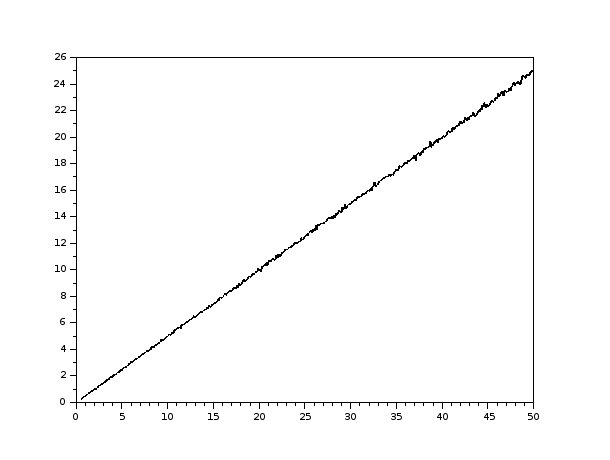
\includegraphics[scale=.5]
      {Figures/ESSEC-I_2018/Figure_ESSEC-I_2018.png}
    \end{center}
    
    
    %\newpage
    
    
    \begin{proof}~
      \begin{noliste}{$\sbullet$}
	\item D'après la question \itbf{5.b)(i)} :
	\[
	  g_n : x \mapsto \left\{
	  \begin{array}{cR{3cm}}
	    \dfrac{n \, \lambda \, x^{n \lambda -1}}{\alpha^{n \lambda}}
	    & si $x \in \ ]0, \alpha[$
	    \nl
	    \nl[-.2cm]
	    0 & sinon
	  \end{array}
	  \right.
	  \quad \text{et} \quad 
	  G_n : x \mapsto \left\{
	  \begin{array}{cR{3cm}}
	    0 & si $x \in \ ]-\infty, 0]$
	    \nl
	    \nl[-.2cm]
	    \dfrac{x^{n \lambda}}{\alpha^{n \lambda}} & si 
	    $x \in \ ]0, \alpha[$
	    \nl
	    \nl[-.2cm]
	    1 & si $x \in [\alpha, +\infty[$
	  \end{array}
	  \right.
	\]
	
	\item Soit $x \in \ ]0,\alpha[$.\\
	D'après le théorème de transfert :
	\[
	  \begin{array}{rcl}
	    \E(\varphi_x(Y_{n-1})) & = & \dint{0}{x} t \, g_{n-1}(t) \dt
	    \ = \ \dint{0}{x} t \, \dfrac{(n-1) \lambda}{\alpha^{(n-1)
	    \lambda}} \, t^{(n-1) \lambda -1} \dt
	    \\[.6cm]
	    & = & \dfrac{(n-1) \lambda}{\alpha^{(n-1) \lambda}} \, 
	    \dint{0}{x} t^{(n-1) \lambda} \dt 
	    \ = \ \dfrac{(n-1) \lambda}{\alpha^{(n-1) \lambda}} \,
	    \Prim{\dfrac{t^{(n-1) \lambda +1}}{(n-1) \lambda +1}}
	    {0}{x}
	    \\[.6cm]
	    & = & \dfrac{(n-1) \lambda}{\alpha^{(n-1) \lambda}} \,
	    \dfrac{x^{(n-1) \lambda +1}}{(n-1) \lambda +1}
	  \end{array}
	\]
	
	\item On en déduit :
	\[
	  \sigma(x) \ = \ \dfrac{\E(\varphi_x(Y_{n-1})}{G_{n-1}(x)}
	  \ = \ \dfrac{\frac{(n-1) \lambda \, x^{\bcancel{(n-1) 
	  \lambda} +1}}{((n-1) \lambda +1) 
	  \bcancel{\alpha^{(n-1) \lambda}}}}
	  {\frac{\bcancel{x^{(n-1) \lambda}}}{\bcancel{
	  \alpha^{(n-1) \lambda}}}} \ = \
	  \dfrac{(n-1) \lambda}{(n-1) \lambda +1} \, x
	\]
	\conc{$\forall x \in \ ]0, \alpha[$, $\sigma(x) = 
	\dfrac{(n-1) \lambda}{(n-1) \lambda +1} \, x$}
	
	\item On a ainsi prouvé que la fonction $\sigma$ est linéaire 
	(de la forme $x \mapsto a \, x$). 
	\conc{Sa courbe représentative est donc 
	une droite passant par l'origine, \\
	ce qui est en accord avec la 
	courbe fournie par l'énoncé.}
      \end{noliste}
      
      ~\\[-1.4cm]
    \end{proof}
  \end{noliste}
\end{noliste}



%\newpage



\section*{Partie III - Modélisation d'enchères}

\noindent
Un bien est mis en vente aux enchères et $n$ acheteurs $A_1$, $\ldots$,
$A_n$ sont intéressés. Chaque acheteur $A_k$ attribue une valeur $x_k$ 
à ce bien, appelée \emph{valeur privée}, qui n'est pas connue des 
autres acheteurs. Afin de se procurer ce bien, $A_k$ propose ensuite, 
de façon secrète, une \emph{mise} (on dit aussi une \emph{offre}) 
$y_k$. Toutes les mises sont alors révélées simultanément et l'acheteur 
qui remporte le bien est celui qui a proposé la plus grande mise. En 
cas d'égalité, le gagnant est tiré au sort parmi ceux qui ont la mise 
la plus importante.\\
Le prix à payer par le gagnant au vendeur dépend du type d'enchère 
organisé. On étudie ici deux formats d'enchères :
\begin{noliste}{$\sbullet$}
  \item l'\emph{enchère au premier prix}, ou enchère hollandaise : 
  l'acheteur gagnant paye la mise qu'il a lui-même proposée. Ce type 
  d'enchère correspond aux enchères dynamiques \og descendantes \fg{} :
  la vente commence avec un prix très élevé et baisse progressivement.
  Le premier qui accepte le prix remporte le bien.
  
  \item l'\emph{enchère au second prix}, ou enchère anglaise : 
  l'acheteur gagnant paye le prix correspondant à la deuxième meilleure
  mise.\\
  Ce type d'enchère est presque équivalent aux enchères dynamiques \og
  montantes \fg{} bien connues : le prix monte progressivement 
  jusqu'à ce qu'il ne reste plus qu'un seul acheteur : celui qui est 
  prêt à mettre le plus haut prix, et qui paye (à peu de chose près) le
  prix de la deuxième offre après la sienne.
\end{noliste}
Pour chaque acheteur $A_k$, on appelle \emph{résultat net} ou 
simplement \emph{résultat} de l'enchère, et on note $r_k$, le bénéfice 
ou le perte résultant de l'opération. Pour l'acheteur qui a remporté 
l'enchère, le résultat est la différence entre la valeur privée et le 
prix payé. Pour les autres acheteurs, le résultat est considéré comme 
nul.\\
À titre d'exemple, considérons quatre acheteurs, dont les mises en 
euros sont $y_1=50$, $y_2=100$, $y_3=80$ et $y_4=40$, alors l'acheteur 
$A_2$ gagne l'enchère. Si sa valeur privée $x_2$ vaut $90$ euros, il 
paye $100$ euros au vendeur pour un résultat de $r_2=-10$ euros s'il 
s'agit d'une enchère au premier prix, et $80$ euros pour un résultat de 
$r_2=10$ euros si c'est une enchère au second prix.\\
On s'intéresse au problème suivant : à partir de l'information dont 
dispose l'acheteur $k$, notamment à partir de sa valeur privée $x_k$, 
comment doit-il choisir sa mise $y_k$ afin d'optimiser son résultat net 
? On appelle \emph{stratégie} de l'acheteur $k$ une fonction $\sigma_k$ 
telle que $y_k = \sigma_k(x_k)$.



\subsection*{1- Enchère au premier prix}

\noindent
On suppose que chaque acheteur $A_k$ a une valeur privée $x_k = 
X_k(\omega)$ qui est une réalisation de la variable aléatoire $X_k$.\\
Soit $\sigma$ la fonction définie à la partie II.\\
Le problème étant symétrique, on se met par exemple à la place de 
l'acheteur $n$, et on suppose que les $n-1$ premiers acheteurs 
appliquent la stratégie $\sigma$, c'est-à-dire : pour tout $k\in \{1, 
\ldots, n-1\}$, l'acheteur $k$ mise $\sigma(X_k)$.\\
L'acheteur $n$ a une valeur privée $x_n$ et choisit une mise $y_n$.\\
On note $E_n$ l'événement \og l'acheteur $A_n$ remporte l'enchère \fg{}.
\begin{noliste}{1.}
  \setlength{\itemsep}{4mm}
  \setcounter{enumi}{9}
  \item En remarquant que $\Prob(\Ev{Y_{n-1} = \sigma^{-1}(y_n)}) = 0$,
  montrer que $\Prob(E_n) = \Prob(\Ev{Y_{n-1} < \sigma^{-1}(y_n)})$.\\
  On note $R_n$ la variable aléatoire donnant le résultat net de 
  l'enchère pour l'acheteur $A_n$.\\
  Justifier que $R_n = (x_n-y_n) \, \unq{}_{E_n}$ et en déduire que le 
  résultat espéré de l'acheteur $A_n$ en fonction de sa valeur 
  privée $x_n \in \ ]0,\alpha[$ et de l'offre $y_n \in \ ]0,\beta[$ 
  est donné par :
  \[
    \E(R_n) \ = \ (x_n-y_n) \, G_{n-1}(\sigma^{-1}(y_n))
  \]
  
  
  %\newpage
  
  
  \begin{proof}~
    \begin{noliste}{$\sbullet$}
      \item L'événement $E_n$ est réalisé si et seulement si 
      l'acheteur $A_n$ remporte l'enchère, c'est-à-dire si sa mise 
      $y_n = \sigma(x_n)$ est :
      \begin{noliste}{$\stimes$}
	\item ou bien strictement supérieure aux mises des 
	$n-1$ autres acheteurs : $\sigma(x_1)$, $\ldots$, 
	$\sigma(x_n)$.\\
	Cet événement s'écrit :
	\[
	  \dcap{k=1}{n-1} \Ev{\sigma(X_k) < y_n}
	  \ = \ \Ev{\max\big( \sigma(X_1), \ldots, \sigma(X_{n-1})\big)
	  < y_n}
	\]
	
	
	\item ou bien égale à une ou plusieurs mises (la plus haute) 
	des $n-1$ 
	autres acheteurs, puis est tirée au sort parmi celles-ci.\\
	Cet événement s'écrit :
	\[
	  \Ev{\max\big( \sigma(X_1), \ldots, \sigma(X_n)\big)
	  = y_n} \cap E_n
	\]
      \end{noliste}
      Finalement :
      \[
        E_n = \Ev{\max(\sigma(X_1) , \ldots, \sigma(X_n)) \leq 
        y_n} \cap E_n
      \]
      
      \item D'après la question \itbf{7.b)}, la fonction $\sigma$
      est strictement croissante sur $]0,\alpha[$, donc :
      \[
        \max(\sigma(x_1), \ldots, \sigma(x_{n-1})) \ = \ 
        \sigma(\max(x_1, \ldots, x_{n-1}))
      \]
      En effet :
      \begin{noliste}{$\stimes$}
	\item d'une part, par définition de $\max(x_1, \ldots, 
	x_{n-1})$ :
	\[
	  \forall i \in \llb 1, n-1 \rrb, \ x_i \leq 
	  \max(x_1, \ldots, x_{n-1})
	\]
	Donc, par croissance de $\sigma$ sur $]0,\alpha[$ :
	\[
	  \forall i \in \llb 1, n-1 \rrb, \ \sigma(x_i) \leq 
	  \sigma\big(\max(x_1, \ldots, x_{n-1})\big)
	\]
	Ceci est valable pour tout $i \in \llb 1, n-1 \rrb$, donc :
	\[
	  \max \big( \sigma(x_1), \ldots, \sigma(x_n)\big) \leq 
	  \sigma\big( \max(x_1, \ldots, x_n)\big)
	\]
	
	\item d'autre part, par définition de $\max\big( \sigma(x_1)
	, \ldots, \sigma(x_{n-1})\big)$ :
	\[
	  \forall i \in \llb 1, n-1 \rrb, \ \sigma(x_i) \leq 
	  \max\big( \sigma(x_1), \ldots, \sigma(x_{n-1})\big)
	\]
	Donc, en particulier :
	\[
	  \sigma\big(\max(x_1, \ldots, x_{n-1})\big) \leq \max\big(
	  \sigma(x_1), \ldots, \sigma(x_{n-1})\big)
	\]
      \end{noliste}
      Finalement, on a bien : $\sigma\big( \max(x_1, \ldots, x_n) \big)
      \ = \ \max\big( \sigma(x_1), \ldots, \sigma(x_n) \big)$.
      
      \item On en déduit :
      \[
       \begin{array}{rcl@{\qquad}>{\it}R{4cm}}
        E_n & = & \Ev{\max\big( \sigma(X_1), \ldots, \sigma(X_{n-1})
        \big) \leq y_n} \cap E_n
        \\[.4cm]
        & = & \Ev{\sigma\big( \max(X_1, \ldots, X_{n-1})
        \big) \leq y_n} \cap E_n
        \\[.4cm]
        & = & \Ev{\sigma(Y_{n-1}) \leq y_n} \cap E_n
        \\[.4cm]
        & = & \Ev{Y_{n-1} \leq \sigma^{-1}(y_n)} \cap E_n
        & (par stricte croissance de $\sigma^{-1}$ sur $]0,\beta[$)
        \nl
        \nl[-.2cm]
        & = & \Ev{Y_{n-1} < \sigma^{-1}(y_n)} \cup \big( \Ev{Y_{n-1} = 
        \sigma^{-1}(y_n)} \cap E_n\big)
       \end{array}
      \]
      
      
      %\newpage
      
      
      \item Par incompatibilité de ces deux événements :
      \[
        \Prob(E_n) \ = \ \Prob(\Ev{Y_{n-1} < \sigma^{-1}(y_n)})
        + \Prob(\Ev{Y_{n-1} = \sigma^{-1}(y_n)} \cap E_n)
      \]
      De plus, d'après la question \itbf{1.b)}, la \var $Y_{n-1}$ est 
      une variable aléatoire à densité, donc :
      \[
        \forall a \in \R, \ \Prob(\Ev{Y_{n-1} = a}) = 0
      \]
      En particulier : $\Prob(\Ev{Y_{n-1} = \sigma^{-1}(y_n)}) 
      =0$.\\[.1cm]
      Or $\Ev{Y_{n-1} = \sigma^{-1}(y_n)} \cap E_n \ \subset \ 
      \Ev{Y_{n-1} = \sigma^{-1}(y_n)}$. Donc :
      \[
        0 \leq \Prob\big(\Ev{Y_{n-1} = \sigma^{-1}(y_n)} \cap E_n 
        \big) \leq \Prob\big(\Ev{Y_{n-1} = \sigma^{-1}(y_n)} \big) =0
      \]
      Ainsi : $\Prob\big(\Ev{Y_{n-1} = \sigma^{-1}(y_n)} \cap E_n
      \big) =0$.
      \conc{On en déduit : $\Prob(E_n) = \Prob(\Ev{Y_{n-1} < 
      \sigma^{-1}(y_n)})$.}
      
      \item D'après l'énoncé :
      \begin{noliste}{$\stimes$}
	\item si l'acheteur $A_n$ remporte l'enchère, alors le 
	résultat $r_n$ de l'enchère est la différence entre la valeur
	privée $x_n$ et le prix payé $y_n$ (car c'est une 
	enchère au premier prix).\\
	Donc, si l'acheteur $A_n$ remporte l'enchère : $r_n = 
	x_n - y_n$.
	
	\item si l'acheteur $A_n$ ne remporte pas l'enchère, le 
	résultat $r_n$ est nul : $r_n=0$.
      \end{noliste}
      
      \item La variable aléatoire $\unq{}_{E_n}$ est définie par :
      \[
        \unq{}_{E_n} : \omega \mapsto \left\{
        \begin{array}{cR{3cm}}
          1 & si $\omega \in E_n$
          \nl
          0 & sinon
        \end{array}
        \right.
      \]
      Soit $\omega \in \Omega$. Deux cas se présentent :
      \begin{noliste}{$\stimes$}
	\item \dashuline{si $\omega \in E_n$}, c'est-à-dire si 
	$E_n$ est réalisé, alors on a montré précédemment : $R_n(\omega)
	=x_n-y_n$.\\
	De plus, par définition de $\unq{}_{E_n}$ : $\unq{}_{E_n}
	(\omega)=1$. Donc :
	\[
	  (x_n-y_n) \, \unq{}_{E_n}(\omega) \ = \ x_n-y_n \ = \
	  R_n(\omega)
	\]
	
	\item \dashuline{si $\omega \in \overline{E_n}$}, c'est-à-dire 
	si $\overline{E_n}$ est réalisé (l'acheteur $A_n$ ne remporte 
	pas l'enchère), alors on a montré : $R_n(\omega)=0$.\\
	De plus, par définition de $\unq{}_{E_n}$ : $\unq{}_{E_n}
	(\omega)=0$ (car $\omega \notin E_n$). Donc :
	\[
	  (x_n-y_n) \, \unq{}_{E_n}(\omega) \ = \ 0 \ = \
	  R_n(\omega)
	\]
      \end{noliste}
      Finalement : $\forall \omega \in \Omega, \ R_n(\omega) = 
      (x_n - y_n) \, \unq{}_{E_n}(\omega)$.
      \conc{D'où : $R_n = (x_n-y_n) \, \unq{}_{E_n}$.}
      
      \item La \var $\unq{}_{E_n}$ admet une espérance car c'est une 
      \var finie. En effet : $\unq{}_{E_n}(\Omega) = \{0,1\}$.\\
      Donc la \var $R_n$ admet une espérance en tant que multiple
      de $\unq{}_{E_n}$.
      
      \item Par définition de l'espérance :
      \[
        \begin{array}{rcl}
          \E(\unq{}_{E_n}) & = & \bcancel{0 \times \Prob(\Ev{\unq{}_{E_n}
          =0})} + 1 \times \Prob(\Ev{\unq{}_{E_n} =1})
          \\[.4cm]
          & = & \Prob(\Ev{\unq{}_{E_n}=1})
        \end{array}
      \]
      Soit $\omega \in \Omega$.
      \[
        \omega \in \Ev{\unq{}_{E_n}=1} \ \Leftrightarrow \
        \unq{}_{E_n}(\omega) = 1 \ \Leftrightarrow \ \omega \in E_n
      \]
      Donc : $\Ev{\unq{}_{E_n}=1} \ = \ E_n$. Ainsi :
      \[
        \E(\unq{}_{E_n}) \ = \ \Prob(\Ev{\unq{}_{E_n} =1}) \ = \
        \Prob(E_n)
      \]
      
      
      %\newpage
      
      
      \item On en déduit :
      \[
        \begin{array}{rcl@{\qquad}>{\it}R{4.5cm}}
          \E(R_n) & = & \E\big( (x_n-y_n) \, \unq{}_{E_n}\big)
          \\[.1cm]
          & = & (x_n-y_n) \, \E(\unq{}_{E_n})
          & (par linéarité de l'espérance)
          \nl
          \nl[-.3cm]
          & = & (x_n-y_n) \, \Prob(E_n)
          \\[.4cm]
          & = & (x_n- y_n) \, \Prob(\Ev{Y_{n-1} < \sigma^{-1}(y_n)})
          \\[.3cm]
          & = & (x_n-y_n) \, G_{n-1}(\sigma^{-1}(y_n))
          & (car $G_{n-1}$ est la fonction de répartition de 
          $Y_{n-1}$)
        \end{array}
      \]
      \conc{$\E(R_n) \ = \ (x_n-y_n) \, 
      G_{n-1}(\sigma^{-1}(y_n))$}~\\[-1cm]
    \end{noliste}
    
    ~\\[-1.4cm]
  \end{proof}
  
  \item En déduire que pour optimiser son espérance de résultat, 
  l'acheteur $A_n$ a intérêt à appliquer lui aussi la stratégie 
  $\sigma$.\\
  Il s'agit de ce que l'on appelle un \emph{équilibre de Nash} en 
  théorie des jeux : si tous les acheteurs appliquent cette 
  stratégie d'équilibre $\sigma$, alors aucun n'a intérêt à 
  changer de stratégie.
  
  \begin{proof}~
    \begin{noliste}{$\sbullet$}
      \item Pour optimiser l'espérance du résultat de $A_n$, il faut
      maximiser la fonction $y_n \mapsto \E(R_n)$, c'est-à-dire la 
      fonction :
      \[
        y \ \mapsto \ (x-y) \, G_{n-1}(\sigma^{-1}(y)) = \gamma(x,y)
      \]
      
      \item Or, d'après la question \itbf{7.b)(iii)}, la fonction 
      $y \mapsto \gamma(x,y)$ est maximale en $\sigma(x)$.\\
      Donc, pour maximiser $\E(R_n)$, l'acheteur $A_n$ doit choisir
      $y_n=\sigma(x_n)$.
    \end{noliste}
    
    \conc{Pour optimiser son espérance de résultat, l'acheteur $A_n$
    doit donc appliquer la stratégie $\sigma$.}~\\[-1.2cm]
  \end{proof}
\end{noliste}



%\newpage



\subsection*{2- Enchère au second prix}

\noindent
On se met à nouveau à la place de l'acheteur $n$. Soit $m = \max(y_1, 
\ldots, y_{n-1})$ la meilleure offre faite par les acheteurs $A_1$, 
$\ldots$, $A_{n-1}$ (que $A_n$ ne connaît pas).
\begin{noliste}{1.}
  \setlength{\itemsep}{4mm}
  \setcounter{enumi}{11}
  \item \begin{noliste}{a)}
    \setlength{\itemsep}{2mm}
    \item Si on suppose que $m \geq x_n$, montrer que quelle que soit la
    mise $y_n$, le résultat net $r_n$ pour $A_n$ est négatif ou nul. 
    Que vaut $r_n$ pour le choix $y_n = x_n$ ?
    
    \begin{proof}~
      \begin{noliste}{$\sbullet$}
	\item L'acheteur $A_n$ remporte l'enchère si et seulement si
	sa mise est supérieure à celle des autres acheteurs, 
	c'est-à-dire : $y_n > m$ ou, $y_n=m$ et il est tiré au sort.\\
	Quatre cas se présentent donc :
	\begin{noliste}{$\stimes$}
	  \item \dashuline{si $y_n > m$}, alors l'acheteur $A_n$
	  remporte l'enchère. Donc $r_n$ est la différence entre 
	  la valeur privée $x_n$ et le prix payé $m$ (car c'est une 
	  enchère au second prix).\\
	  Donc, si $A_n$ remporte l'enchère : $r_n = x_n -m$.\\
	  Or on suppose : $m \geq x_n$. Donc $r_n \leq 0$.
	  
	  \item \dashuline{si $y_n=m$ et $A_n$ est tiré 
	  au sort}, alors l'acheteur $A_n$ remporte l'enchère.\\
	  Donc on a toujours : $r_n \leq 0$.
	  
	  \item \dashuline{si $y_n=m$ et $A_n$ n'est pas tiré 
	  au sort}, alors il ne remporte pas 
	  l'enchère. Donc $r_n=0$.
	  
	  \item \dashuline{si $y_n <m$}, alors l'acheteur $A_n$ ne 
	  remporte pas l'enchère. Donc $r_n=0$.
	\end{noliste}
	\conc{Finalement, quelle que soit la mise $y_n$, on obtient :
	$r_n \leq 0$.}
	
	\item Si $y_n =x_n$, quatre cas se présentent :
	\begin{noliste}{$\stimes$}
	  \item \dashuline{si $y_n > m$} :
	  \[
	    r_n \ = \ x_n-m \ = \ y_n - m \ \geq \ 0
	  \]
	  Or, d'après précédemment : $r_n \leq 0$. Donc : $r_n=0$.
	  
	  \item \dashuline{si $y_n=m$ et $A_n$ est tiré 
	  au sort}, on obtient de même : $r_n=0$.
	  
	  \item \dashuline{si $y_n=m$ et $A_n$ n'est pas tiré 
	  au sort}, alors : $r_n=0$.
	  
	  \item \dashuline{si $y_n <m$}, alors : $r_n=0$.
	\end{noliste}
	\conc{Finalement, si $y_n = x_n$, alors $r_n=0$.}~\\[-1.4cm]
      \end{noliste}
    \end{proof}

    
    \item Si on suppose que $m < x_n$, quel est le résultat pour $A_n$
    dans les cas $y_n < m$ et $y_n \geq m$ ?
    
    \begin{proof}~\\
      Dans cette question, on suppose : $m < x_n$. Deux cas se 
      présentent :
      \begin{noliste}{$\stimes$}
	\item \dashuline{si $y_n < m$}, alors l'acheteur $A_n$ ne 
	remporte pas l'enchère. \\
	Donc : $r_n=0$.
	
	\item \dashuline{si $y_n \geq m$}, alors l'acheteur $A_n$
	remporte l'enchère.\\
	Donc : $r_n= x_n-m$.
      \end{noliste}
      \conc{Si $m<x_n$, alors : $r_n = \left\{
      \begin{array}{cR{3cm}}
        0 & si $y_n < m$
        \nl
        x_n-m & si $y_n \geq m$
      \end{array}
      \right.$.}
      
      ~\\[-1.4cm]
    \end{proof}

    
    %\newpage
    
    
    \item En déduire que la meilleure stratégie pour $A_n$ consiste 
    à prendre $y_n =x_n$.
    
    \begin{proof}~\\
      Deux cas se présentent :
      \begin{noliste}{$\sbullet$}
	\item \dashuline{si $m \geq x_n$}.\\[.1cm]
	D'après la question \itbf{12.a)} : $r_n \leq 0$.\\
	De plus, si $y_n = x_n$, alors $r_n=0$.\\
	Ainsi, la meilleure stratégie pour l'acheteur $A_n$ est de 
	choisir $y_n = x_n$.
	
	\item \dashuline{si $m< x_n$}.
	\begin{noliste}{-}
	  \item D'après la question \itbf{12.b)} : $r_n = \left\{
	  \begin{array}{cR{3cm}}
	    0 & si $y_n < m$
	    \nl
	    x_n-m & si $y_n \geq m$
	  \end{array}
	  \right.$\\[.2cm]
	  Or $x_n-m >0$. Donc, si $y_n \geq m$, alors $r_n >0$.
	  
	  \item Ainsi, la meilleure stratégie pour l'acheteur $A_n$
	  est donc de choisir une mise $y_n$ telle que $y_n \geq m$.\\
	  Dans ce cas, quelle que soit la mise $y_n$, $r_n=x_n-m$.
	  
	  \item Or : $x_n >m$. Donc, en choisissant $y_n = x_n$, on 
	  est dans le cas $y_n \geq m$. Ainsi : $r_n = x_n-m>0$.
	\end{noliste}
	On en déduit qu'une stratégie optimale pour $A_n$ est de 
	choisir $y_n =x_n$.
      \end{noliste}
      \conc{Finalement, dans tous les cas, une stratégie optimale 
      pour $A_n$ est de choisir $y_n=x_n$.}~\\[-1.2cm]
    \end{proof}
  \end{noliste}
\end{noliste}
Par symétrie, chaque acheteur a également intérêt à miser le montant de 
sa valeur privée. On parle de \emph{stratégie dominante} : chaque 
acheteur a une stratégie optimale indépendamment du comportement des 
autres acheteurs.




\subsection*{3- Équivalence des revenus}


\noindent
On se met maintenant à la place du vendeur.\\
Les valeurs privées des acheteurs sont données par les variables 
aléatoires $X_1$, $\ldots$, $X_n$.
\begin{noliste}{1.}
  \setlength{\itemsep}{4mm}
  \setcounter{enumi}{12}
  \item Enchère au premier prix.\\
  On suppose que le vendeur organise une enchère au premier prix, et 
  que les acheteurs adoptent la stratégie d'équilibre $\sigma$ donnée
  à la partie III-1.\\
  On note $B_n$ la variable aléatoire donnant le \emph{bénéfice}, ou 
  \emph{revenu}, du vendeur. Il s'agit du montant que paye l'acheteur
  qui a remporté l'enchère.
  \begin{noliste}{a)}
    \setlength{\itemsep}{2mm}
    \item Justifier que $B_n = \sigma(Y_n)$.
    
    \begin{proof}~
      \begin{noliste}{$\sbullet$}
	\item L'acheteur ayant la mise maximale remporte l'enchère et
	paye donc $\max(y_1, \ldots, y_n)$ (car c'est une enchère au 
	premier prix).
	
	\item Or, chaque acheteur adopte la stratégie $\sigma$. Donc :
	$\forall i \in \llb 1,n \rrb$, $y_i = \sigma(x_i)$.\\
	L'acheteur gagnant paye donc $\max\big(\sigma(x_1), \ldots,
	\sigma(x_n)\big)$.
	
	\item De plus, par croissance de $\sigma$ sur $]0,\alpha[$ :
	\[
	  \max\big( \sigma(x_1), \ldots, \sigma(x_n)\big) \ = \
	  \sigma\big(\max(x_1, \ldots, x_n)\big)
	\]
	{\it (la démonstration de cette égalité est détaillée en 
	question \itbf{10.})}
	
	\item On en déduit que l'acheteur gagnant paye 
	$\sigma\big(\max(x_1, \ldots, x_n)\big)$.
      \end{noliste}
      \conc{Ainsi : $B_n = \sigma\big(\max(X_1, \ldots, X_n)\big)
      = \sigma(Y_n)$.}~\\[-1cm]
    \end{proof}
    
    
    %\newpage

    
    \item En déduire :
    \[
      \E(B_n) \ = \ n \, \dint{0}{\alpha} \sigma(x) \, G_{n-1}(x) \,
      f(x) \dx \ = \ n \, \dint{0}{\alpha} \left( \dint{0}{x} t \, 
      g_{n-1}(t) \dt \right) f(x) \dx
    \]
    
    \begin{proof}~
      \begin{noliste}{$\sbullet$}
	\item La fonction $g_n$ est nulle en dehors de $]0,\alpha[$.\\
	Donc, d'après le théorème de transfert, la \var $B_n = 
	\sigma(Y_n)$ admet une espérance si et seulement si 
	l'intégrale $\dint{0}{\alpha} \sigma(x) \, g_n(x) \dx$ est 
	absolument convergente.\\
	Les fonctions $\sigma$ et $g_n$ étant à valeurs positives sur 
	$]0,\alpha[$, cela revient à démontrer que cette intégrale est 
	convergente.
	
	\item La fonction $x \mapsto \sigma(x) \, g_n(x)$ est continue
	par morceaux sur $[0,\alpha]$ (d'après la question 
	\itbf{6.d)}), donc l'intégrale $\dint{0}{
	\alpha} \sigma(x) \, g_n(x) \dx$ est bien définie.
	\conc{Ainsi, la \var $B_n = \sigma(Y_n)$ admet une 
	espérance.}
	
	\item Soit $x \in \ ]0,\alpha[$.
	\[
	  \begin{array}{rcl@{\qquad}>{\it}R{4.5cm}}
	    \sigma(x) \, g_n(x) & = & n \, \sigma(x) \, f(x) \, 
	    (F(x))^{n-1}
	    & (d'après la question \itbf{1.b)})
	    \nl
	    \nl[-.2cm]
	    & = & n \, \sigma(x) \, f(x) \, G_{n-1}(x)
	    & (d'après la question \itbf{1.a)})
	  \end{array}
	\]
	\conc{Donc : $\E(B_n) \ = \ \E(\sigma(Y_n)) \ = \ \dint{0}
	{\alpha} \sigma(x) \, g_n(x) \dx \ = \ n \, \dint{0}{\alpha}
	\sigma(x) \, f(x) \, G_{n-1}(x) \dx$.}
	
	\item D'après l'expression $(*)$ en question \itbf{6.d)} :
	\[
	  \forall x \in \ ]0,\alpha[, \ \sigma(x) = 
	  \dfrac{1}{G_{n-1}(x)} \, \dint{0}{x} t \, g_{n-1}(t) \dt
	\]
	D'où : $\forall x \in \ ]0,\alpha[$, $\sigma(x) \, 
	G_{n-1}(x) = \dint{0}{x} t \, g_{n-1}(t) \dt$.\\[.2cm]
	Ainsi : $\dint{0}{\alpha} \sigma(x) \, G_{n-1}(x) \,
	f(x) \dx \ = \ \dint{0}{\alpha} \left(\dint{0}{x} t \,
	g_{n-1}(t) \dt\right) \, f(x) \dx$.
	\conc{$\E(B_n) \ = \ n \, \dint{0}{\alpha} \sigma(x) \, 
	G_{n-1}(x) \, f(x) \dx \ = \ n \, \dint{0}{\alpha} \left(
	\dint{0}{x} t \, g_{n-1}(t) \dt \right) \, f(x) \dx$}~\\[-1.4cm]
      \end{noliste}
    \end{proof}

    
    \item Montrer, à l'aide d'une intégration par parties :
    \[
      \E(B_n) \ = \ n \, \dint{0}{\alpha} x \, (1-F(x)) \, 
      g_{n-1}(x) \dx
    \]
    
    \begin{proof}~
      \begin{noliste}{$\sbullet$}
	\item D'après la question précédente :
      \[
        \E(B_n) \ = \ n \, \dint{0}{\alpha} \left(\dint{0}{x} t \,
        g_{n-1}(t) \dt \right) f(x) \dx
      \]
      \item Soit $(a,b) \in \ ]0, \alpha[^2$ tels que $a \leq b$. On 
      procède par intégration par parties (IPP).
      \[
        \renewcommand{\arraystretch}{2}
        \begin{array}{|rcl@{\qquad}rcl}
          u(x) & = & \dint{0}{x} t \, g_{n-1}(t) \dt & u'(x) & = & 
          x \, g_{n-1}(x) \\
          v'(x) & = & f(x) & v(x) & = & -(1-F(x))
        \end{array}
        \]
      Cette IPP est valide car les fonctions $u$ et $v$ sont de classe
      $\Cont{1}$ sur $[a, b]$.
      
      
      %\newpage
      
      
      On obtient alors :
      \[
        \begin{array}{cl}
          & \dint{a}{b} \left(\dint{0}{x} t \, g_{n-1}(t) \dt\right)
          \, f(x) \dx
          \\[.6cm]
          =& \Prim{-\left(\dint{0}{x} t \, g_{n-1}(t) \dt \right)
          (1-F(x))}{a}{b} + \dint{a}{b} x \, g_{n-1}(x) \, (1-F(x)) \dx
        \end{array}
      \]
      Or :
      \[
       \begin{array}{cl}
        & \Prim{-\left(\dint{0}{x} t \, g_{n-1}(t) \dt \right)
          (1-F(x))}{a}{b} 
        \\[.6cm] 
        = &
        - \left(\dint{0}{b} t \, g_{n-1}(t) \dt \right) \, 
          (1-F(b)) + \left(\dint{0}{a} t \, g_{n-1}(t) \dt \right) \,
          (1-F(a))
       \end{array}
      \]
      De plus, comme la densité $f$ est nulle en dehors de $]0,\alpha[$ 
      :
      \begin{noliste}{$\stimes$}
	\item d'une part $\dlim{a\to 0} F(a) \ = \ F(0) \ = \
	\dint{-\infty}{0} f(t) \dt \ = \ 0$,
	
	\item d'autre part $\dlim{b\to \alpha} F(b) \ = \ F(\alpha) \ = 
	\ \dint{-\infty}{\alpha} f(t) \dt \ = \ 
	\dint{0}{\alpha} f(t) \dt \ = \ 1$
      \end{noliste}
      Enfin :
      \[
        \dlim{a\to 0} \dint{0}{a} t \, g_{n-1}(t) \dt = 0 \qquad 
        \text{et} \qquad \dlim{b\to \alpha} \dint{0}{b} t \, g_{n-1}(t) 
        \dt = \dint{0}{\alpha} t \, g_{n-1}(t) \dt = 
        \E(Y_{n-1})
      \]
      \item Ainsi : 
      \[
        \dint{0}{\alpha} \left(\dint{0}{x} t \, g_{n-1}(t) \dt \right)
        \, f(x) \dx \ = \ -\bcancel{\E(Y_{n-1}) \times (1-1)} + 
        \bcancel{0 \times (1-0)} + \dint{0}{\alpha} x \, (1-F(x))
        \, g_{n-1}(x) \dx
      \]
      \end{noliste}
      \conc{On en déduit : $\E(B_n) \ = \ n \, \dint{0}{\alpha} x \, 
      (1-F(x)) \, g_{n-1}(x) \dx$.}
      
      ~\\[-1.4cm]
    \end{proof}
  \end{noliste}
  
  \item Enchère au second prix.\\
  On suppose que le vendeur organise une enchère au second prix, et que 
  les acheteurs adoptent la stratégie dominante de la partie III-2 : 
  chacun mise autant que sa valeur privée.\\
  On note $B_n'$ la variable aléatoire donnant le revenu du vendeur 
  dans cette enchère.\\
  Justifier que $\E(B_n') = \E(Z_n)$.
  
  \begin{proof}~
   \begin{noliste}{$\sbullet$}
    \item L'acheteur ayant la mise maximale emporte l'enchère. Dans une 
    enchère au second prix, il paye la deuxième mise la plus élevée
    parmi $y_1$, $\ldots$, $y_n$.
    
    
    %\newpage
    
    
    \item Or, avec la stratégie de la question \itbf{12.c)} : 
    $\forall i \in \llb 1, n \rrb$, $y_i=x_i$.\\[.2cm]
    Donc l'acheteur gagnant paye la deuxième plus grande valeur parmi
    $x_1$, $\ldots$, $x_n$.
    \conc{Ainsi : $B_n'=Z_n$.}
    
    
    
    \item La \var $Z_n$ admet une espérance par critère de comparaison 
    des intégrales généralisées de fonctions continues positives (même 
    démonstration qu'en question \itbf{1.c)}).
    \conc{Ainsi, la \var $B_n'$ admet une espérance et : $\E(B_n')
    =\E(Z_n)$.}~\\[-1.4cm]
   \end{noliste}
  \end{proof}

  
  \item Établir : $\E(B_n) = \E(B_n')$.
  
  \begin{proof}~
    \begin{noliste}{$\sbullet$}
      \item D'après la question \itbf{2.b)} : 
      \[
       \begin{array}{rcl}
        \E(Z_n) & = & \dint{0}{\alpha} x \, h_n(x) \dx \ = \
        \dint{0}{\alpha} x \, n(n-1) \, f(x) \, (1-F(x)) \, (F(x))^{n-2}
        \dx
        \\[.6cm]
        & = & n \, \dint{0}{\alpha} x \, (1-F(x)) \, (n-1) \, f(x) \,
        (F(x))^{n-2} \dx
       \end{array}
      \]
      
      \item D'autre part, d'après la question \itbf{1.b)} : 
      \[
        \forall x \in \ ]0, \alpha[, \ g_{n-1}(x) = (n-1) \, f(x) \,
        (F(x))^{n-2}
      \]
      D'où :
      \[
        \E(Z_n) \ = \ n \, \dint{0}{\alpha} x \, (1-F(x)) \, g_{n-1}(x)
        \dx \ = \ \E(B_n)
      \]
    \end{noliste}
    \conc{Ainsi : $\E(B_n') \ = \ \E(Z_n) \ = \ \E(B_n)$.}~\\[-1cm]
  \end{proof}
\end{noliste}
Ainsi, le revenu moyen pour le vendeur est le même pour les enchères au 
premier ou au second prix lorsque les acheteurs adoptent tous la 
stratégie optimale. Plus généralement, on peut montrer que ce revenu 
moyen est encore le même dans une très grande classe de formats 
d'enchères, ce résultat portant le nom de \emph{principe d'équivalence 
du revenu}.






\end{document}
